\documentclass{article} % loại tài liệu
\usepackage[utf8]{vietnam} % tiếng Việt
\usepackage[left = 3.5cm,right = 2cm,top = 3.5cm,bottom = 3cm]{geometry} % căn lề
\usepackage{tikz} % vẽ hình
\usetikzlibrary{calc} % tính toán vẽ hình
\usepackage{graphicx} % hình ảnh
\usepackage{pdfpages} % thêm file pdf bao_cao_tien_do

% Sử dụng gói color để thay đổi màu
\usepackage{color} %* mau_sac
% Sử dụng gói xcolor để mở rộng tính năng thay đổi màu
\usepackage{xcolor} %* mau_sac
% \definecolor{HustRed}{RGB}{206,22,40}
% \definecolor{HustYellow}{RGB}{242,193,8}
\definecolor{BackgroundCode}{RGB}{242,242,235}

% Sử dụng gói caption để tùy chỉnh caption
\usepackage{caption}%* caption
% Sử dụng gói listing để hiển thị mã nguồn
\usepackage{listing}
% \renewcommand*{\listlistingname}{Danh sách mã nguồn}
\DeclareCaptionLabelFormat{code_caption}{{Mã nguồn #2}}
\captionsetup*[listing]{labelformat = code_caption}

% Sử dụng gói minted để đính kèm và định dạng mã nguồn
\usepackage{minted} %! code_python
\setminted{
fontsize = \footnotesize, % Cỡ chữ cho mã nguồn
frame = lines, % Hiển thị đường viền xung quanh mã nguồn
framesep = 2mm, % Khoảng cách giữa đường viền và nội dung mã nguồn
bgcolor = BackgroundCode, % Màu nền cho mã nguồn
linenos, % Hiển thị số dòng ở bên trái
autogobble, % Tự động loại bỏ khoảng trắng ở đầu mỗi dòng
}

\begin{document} % bắt đầu
%%%%%%%%%%%%%%%%%%%%%%%%%%%%%%%%%%%%%

% \begin{titlepage}
\begin{tikzpicture}[remember picture, overlay]
\draw [line width = 3pt]
($ (current page.north west) + (3.0cm, - 2.5cm)$)
rectangle
($ (current page.south east) + (- 2.5cm, 2.5cm)$);
\draw [line width = 0.5pt]
($ (current page.north west) + (3.1cm, - 2.6cm)$)
rectangle
($ (current page.south east) + (- 2.6cm, 2.6cm)$);
\end{tikzpicture}
\begin{center}
\vspace{- 0.4cm}
\textbf{ĐẠI HỌC BÁCH KHOA HÀ NỘI} \\
\textbf{VIỆN TOÁN ỨNG DỤNG VÀ TIN HỌC} \\
\textbf{******}
\vspace{0.8cm}

\begin{figure}[h]
\centering

\includegraphics[scale = .5]{pictures/logoBK.png}
\end{figure}
\vspace{0.7cm}
\textbf{\fontsize{16pt}{30pt}\selectfont {BÁO CÁO ĐỒ ÁN II}} \\
\vspace{1cm}
\textbf{\fontsize{20pt}{24pt}\selectfont {ĐỀ TÀI:}} \\
\textbf{\fontsize{19pt}{24pt}\selectfont {Xây dựng kiến trúc vi dịch vụ cho bài toán hóa đơn điện tử}} \\
% \textbf{\fontsize{20pt}{24pt}\selectfont {Sử dụng thiết kế hướng miền xây dựng kiến trúc vi dịch vụ cho bài toán hóa đơn điện tử}} \\
\end{center}
\vspace{0.7cm}

\hspace{2.4cm}
\begin{minipage}{0.8\textwidth}
\textbf{Giảng viên hướng dẫn: TS. Vũ Thành Nam}
\end{minipage}

\hspace{3cm}
\begin{minipage}{0.7\textwidth}
\begin{tabular}{l l l}
Sinh viên thực hiện & Vũ Văn Nghĩa \\
Mã số sinh viên & 20206205 \\
Lớp & Toán Tin 02 - K65 \\
\end{tabular}
\end{minipage}

\hspace{2.4cm}
\begin{center}
\textbf{\fontsize{20pt}{24pt}\selectfont {Chuyên ngành: Toán Tin}}
\end{center}

\vspace{0.5cm}
\begin{center}
\textbf{Hà Nội, \the\month - \the\year}
\end{center}
\end{titlepage}


% % Trang trắng không có nội dung và không có số trang
\pagestyle{empty}
\thispagestyle{empty}

\mbox{} % Một hộp rỗng để trang không bị trắng toàn bộ

% \newpage

\begin{center}
{\bfseries NHẬN XÉT CỦA GIẢNG VIÊN HƯỚNG DẪN}
\end{center}

\begin{enumerate}
\item Mục đích và nội dung của đồ án:
\vspace{20ex} % Thêm khoảng cách dọc
\item 	Kết quả đạt được:
\vspace{20ex} % Thêm khoảng cách dọc
\item 	Ý thức làm việc của sinh viên:
\vspace{20ex} % Thêm khoảng cách dọc
\end{enumerate}

\hspace{0.4\textwidth}
\begin{minipage}{0.5\textwidth}
\noindent\begin{center}
\textit{Hà Nội, \today} \\
\textbf{Giảng viên hướng dẫn} \\
\textit{(Ký và ghi rõ họ tên)}
\end{center}
\end{minipage}

\pagestyle{empty}

\newpage

% 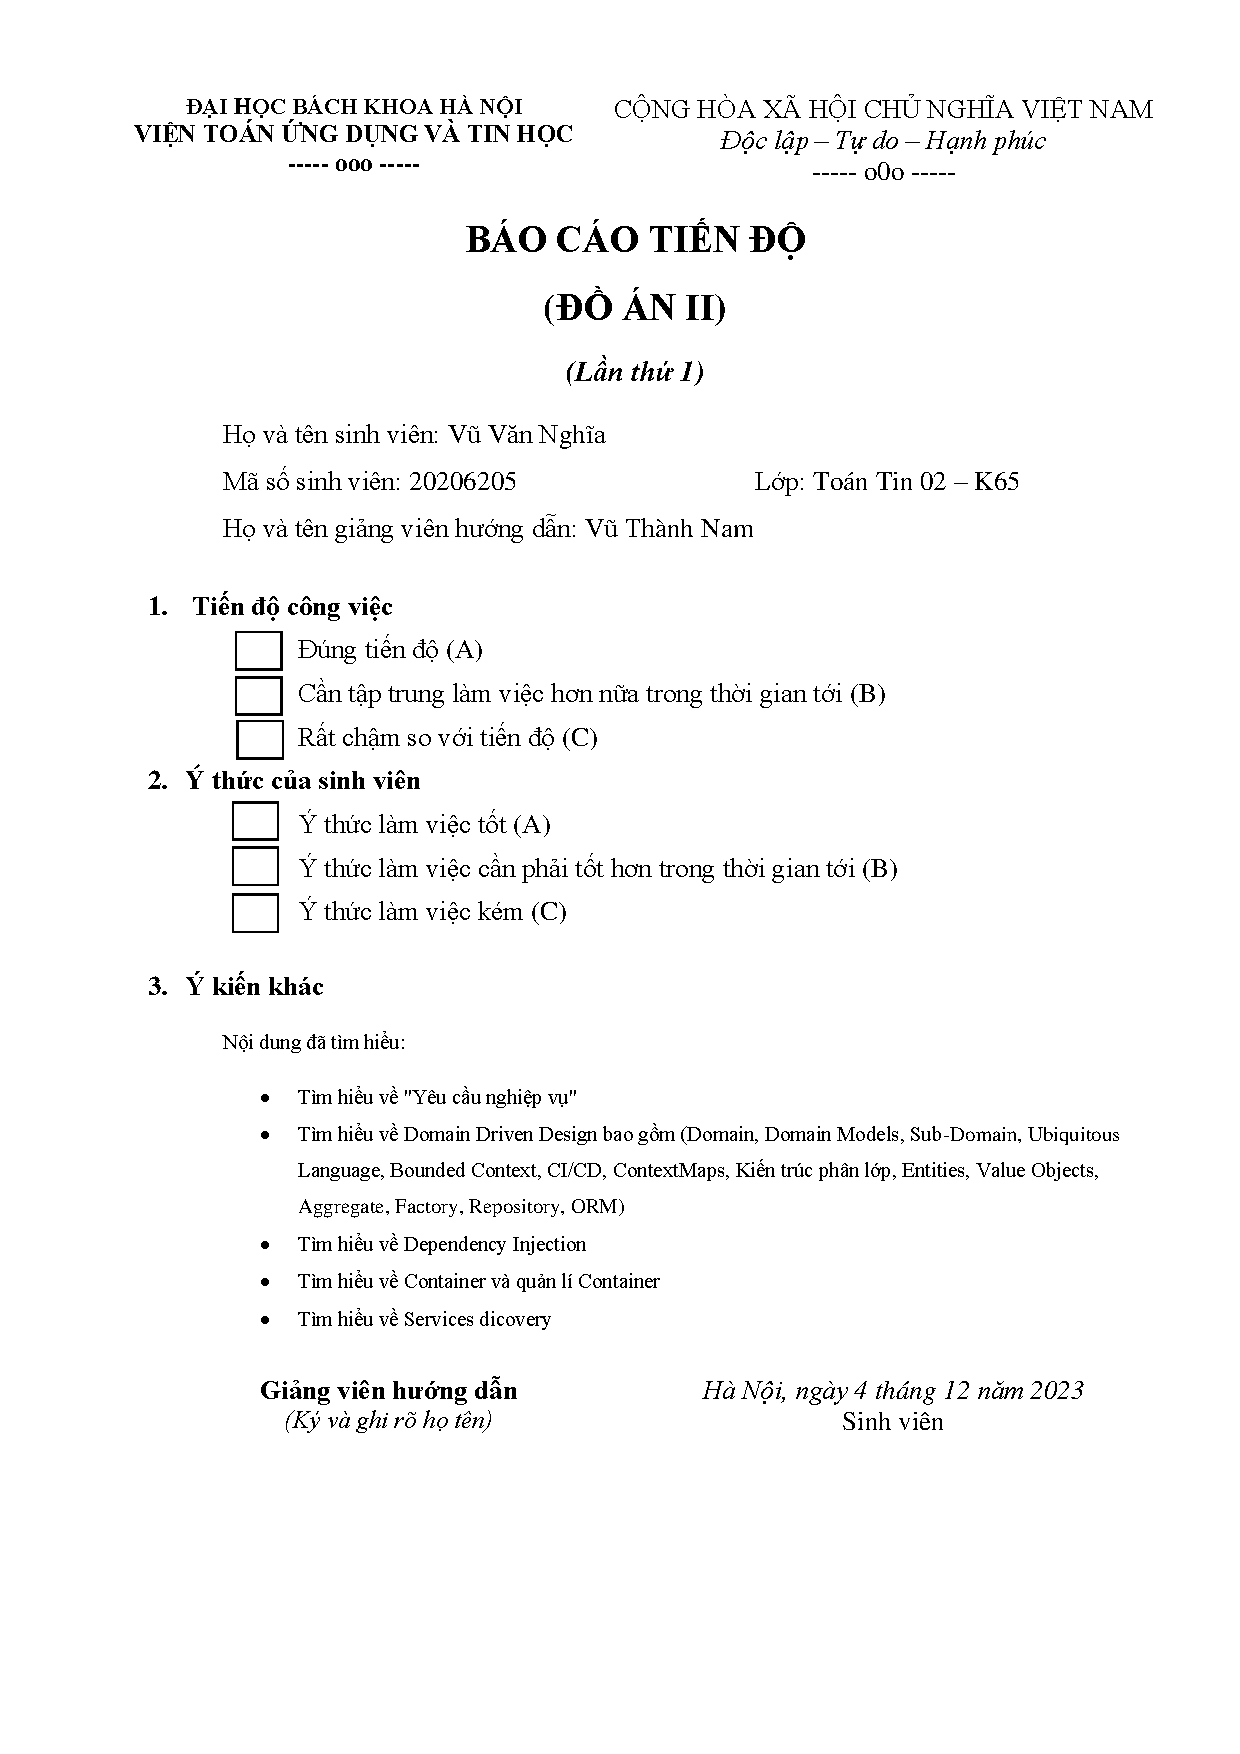
\includepdf[pages = -]{contents/bao_cao_tien_do_1.pdf}
% 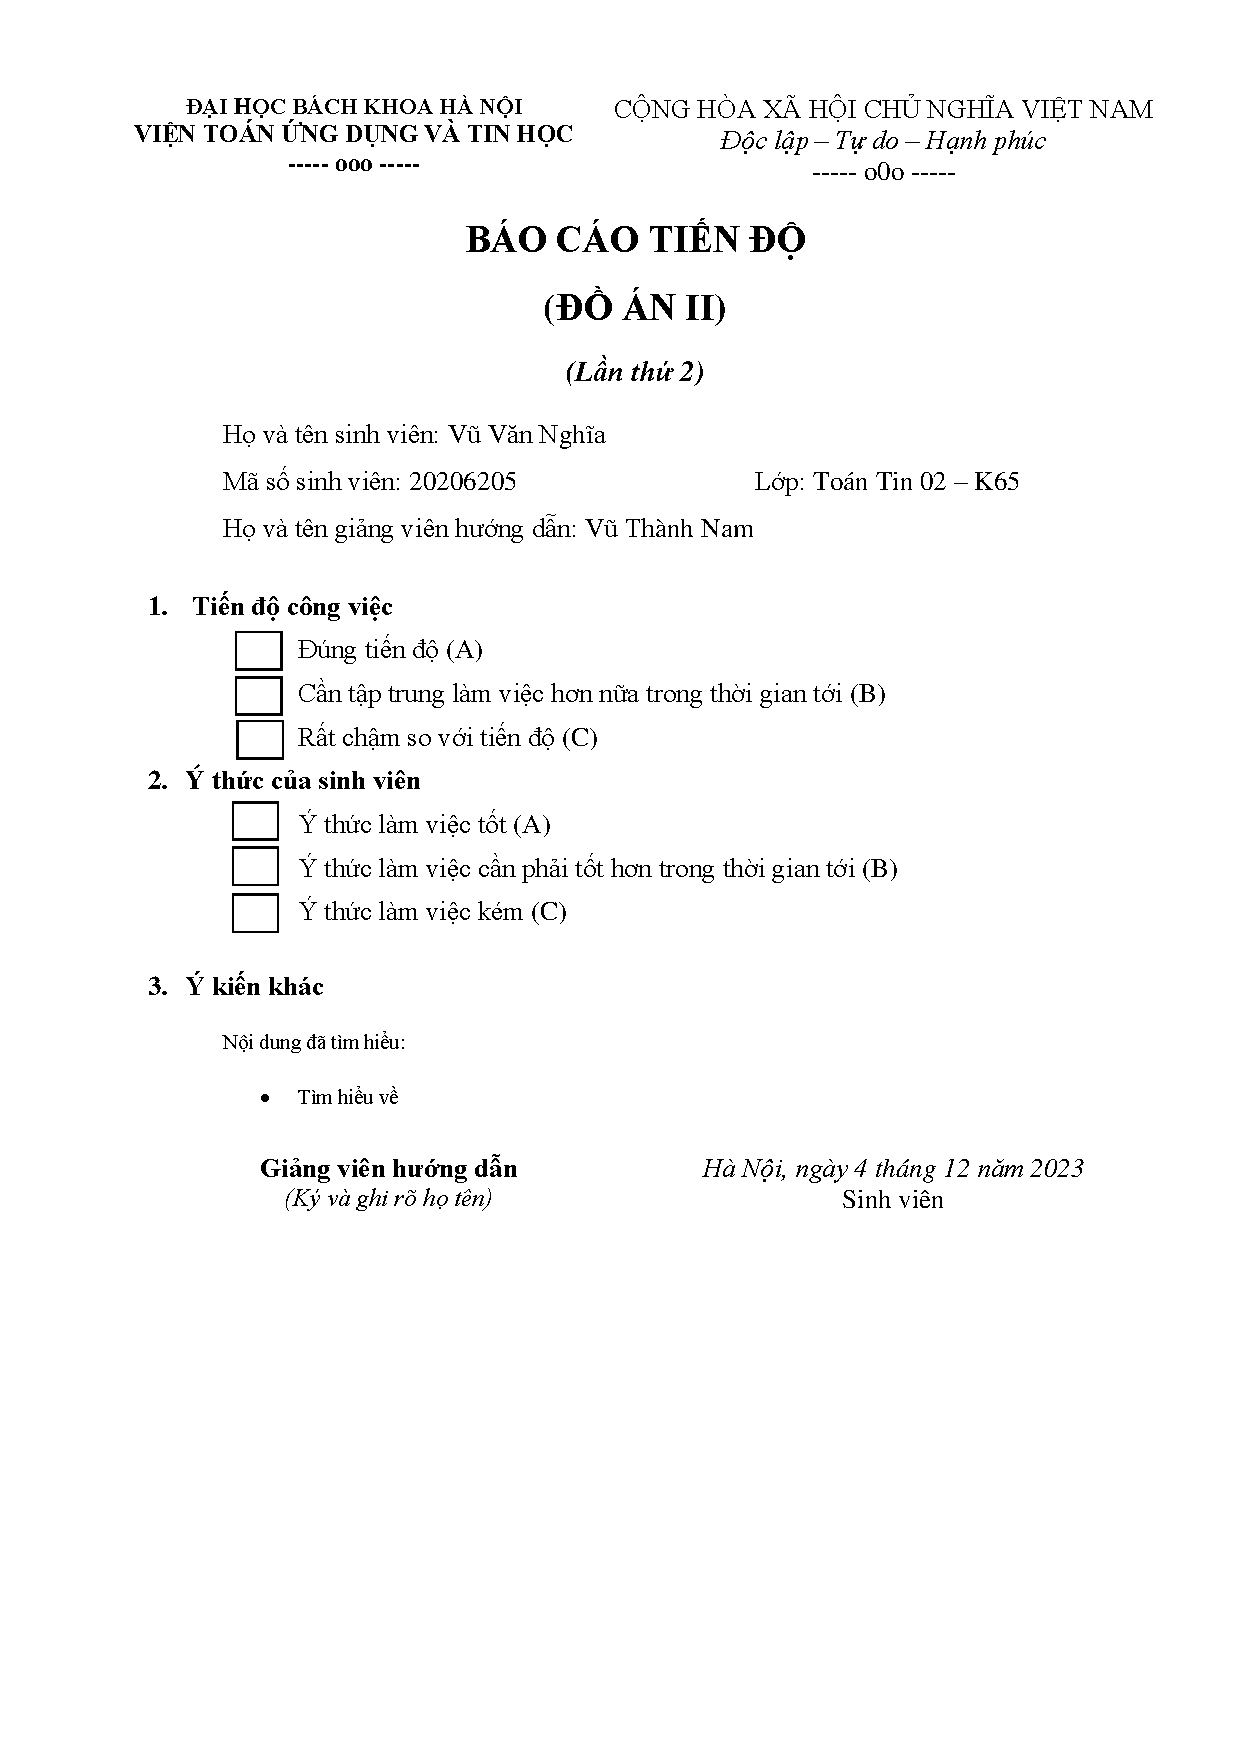
\includepdf[pages = -]{contents/bao_cao_tien_do_2.pdf}

% \newpage
\renewcommand*\contentsname{\centering MỤC LỤC}
\tableofcontents
\newpage



% \newpage

\section*{\centering LỜI CẢM ƠN}

\addcontentsline{toc}{section}{LỜI CẢM ƠN}

\newpage



% \newpage

\section*{\centering LỜI MỞ ĐẦU}

\addcontentsline{toc}{section}{LỜI MỞ ĐẦU}

\newpage

% \newpage
\section*{\centering TÓM TẮT NỘI DUNG ĐỒ ÁN}
\addcontentsline{toc}{section}{TÓM TẮT NỘI DUNG ĐỒ ÁN}
\newpage

% \newpage
\section*{\centering ĐÁNH GIÁ VÀ THẢO LUẬN}
\addcontentsline{toc}{section}{ĐÁNH GIÁ VÀ THẢO LUẬN}
\newpage

% \newpage
\section*{\centering DANH SÁCH BẢNG}
\addcontentsline{toc}{section}{DANH SÁCH BẢNG}
\makeatletter
\renewcommand\listoftables{            
\@starttoc{lot}            
}
\makeatother 
\listoftables  
\newpage

% \newpage
\section*{\centering DANH SÁCH HÌNH ẢNH}
\addcontentsline{toc}{section}{DANH SÁCH HÌNH ẢNH}
\makeatletter
\renewcommand\listoffigures{      
\@starttoc{lof}      
}
\makeatother
\listoffigures  
\newpage

% \newpage

\section*{\centering DANH SÁCH MÃ NGUỒN}

\addcontentsline{toc}{section}{DANH SÁCH MÃ NGUỒN}

\makeatletter

\renewcommand\listoflistings{

\@starttoc{lol}

}

\makeatother

\listoflistings

\newpage

% \newpage
\section*{\centering DANH SÁCH CÁC CỤM TỪ VIẾT TẮT}
\addcontentsline{toc}{section}{DANH SÁCH CÁC CỤM TỪ VIẾT TẮT}

% @sau

\begin{table}[h]
\centering
\begin{tabular}{|c|c|c|c|}
\hline
STT & Từ viết tắt & Từ viết đầy đủ & Mô tả \\
\hline
Dong1 & Dong1 & Cot1 & Cot2 \\
\hline
Dong2 & Dong2 & Cot1 & Cot2 \\
\hline
\end{tabular}
\caption{ViDuBangThuong}
\end{table}

\newpage

% API; Application Programming Interface; Giao diện lập trình ứng dụng
% CI/CD; Continuous Integration (CI) and Continuous Delivery (CD) ; Quá trình tích hợp và chuyển giao liên tục
% thiết kế hướng miền ; thiết kế hướng miền; Kỹ thuật thiết kế theo hướng miền
% DI; Dependency Injection; Cơ chế tiêm sự phụ thuộc giữa các đối tượng
% HTTP; Hypertext Transfer Protocol; Giao thức truyền tải siêu văn bản
% JSON; JavaScript Object Notation; Một kiểu dữ liệu mở rộng của JavaScript
% ORM; Object Relational Mapping; Một kỹ thuật ánh xạ các đối tượng lập trình với từng bảng trong CSDL quan hệ
% Cơ sở dữ liệu ; CSDL ;
% Tạo (Create), Đọc (Read), Sửa (Update), Xóa (Delete) ; CRUD ;
% Kubernetes ; K8s ; kubernetes
% Số điện thoại ; SĐT ;
% UML
% MVC; Model View Controller; Một mẫu thiết kế ứng dụng
% SQL

SOA; Service Oriented Architecture; Kiến trúc hướng dịch vụ
SOAP; Simple Object Access Protocol; Một giao thức để truy cập dịch vụ web
SPA; Single Page Application; Kiểu ứng dụng một trang
REST; Representational State Transfer; Một tiêu chuẩn thiết kế các API sử dụng cho các dịch vụ web
URL; Uniform Resource Locator ; Địa chỉ định vị tài nguyên trên Internet
XML; Extensible Markup Language; Ngôn ngữ đánh dấu mở rộng

% TCT ; TCT ;
Người nộp thuế ; NNT ;
Mã số thuế ; MST ;
Hóa đơn điện tử ; HĐĐT ;
Cơ quan thuế ; CQT ;
Công nghệ thông tin ; CNTT ;



% % STT; Tiếng Anh; Tiếng Việt
% @sau

% kiến trúc nguyên khối, kiến trúc nguyên khối
% kiến trúc nguyên khối, kiến trúc nguyên khối
% kiến trúc vi dịch, kiến trúc vi dịch
% kiến trúc vi dịch, kiến trúc vi dịch
% kiến trúc vi dịch, kiến trúc vi dịch
% kiến trúc vi dịch, kiến trúc vi dịch
% thiết kế hướng miền, thiết kế hướng miền
% thiết kế hướng miền, thiết kế hướng miền

1 thiết kế hướng miền
Thiết kế hướng lĩnh vực
2 Domain (không dịch)
3 Abstraction Trừu tượng
4 chuyên gia ngành

%%%%%%%%%%%
% \section{Giới thiệu}

% Trong thời đại ngày nay, nhu cầu phát triển ứng dụng và hệ thống ngày càng tăng, đặt ra thách thức đối với kiến trúc phần mềm. Kiến trúc nguyên khối đã phục vụ hiệu quả trong quá khứ, nhưng kiến trúc này bắt đầu gặp khó khăn đối mặt với sự phức tạp, khả năng mở rộng và khả năng đáp ứng linh hoạt với thay đổi nhanh chóng trong yêu cầu kinh doanh.

Kiến trúc vi dịch vụ là giải pháp cho những thách thức trên. Kiến trúc vi dịch vụ chia dự án thành những dịch vụ nhỏ độc lập, mỗi dịch vụ chịu trách nhiệm về một chức năng cụ thể. Từ đó, giảm sự phức tạp của dự án tăng tính linh hoạt và dễ dàng quản lý.

Việc vận dụng kết hợp giữa kiến trúc vi dịch vụ và thiết kế hướng miền là một cách tiếp cận toàn diện, giúp xác định và tổ chức các dịch vụ dựa trên việc hiểu rõ về lĩnh vực kinh doanh. Thiết kế hướng miền xây dựng mô hình dựa trên yêu cầu nghiệp vụ thực tế, từ đó dự án phản ánh đúng các quy trình kinh doanh.

% \subsection{Giới thiệu về bài toán hóa đơn điện tử}

% Bài toán hóa đơn điện tử là một phần quan trọng của quá trình chuyển đổi số. Trong quá khứ, mọi người thường sử dụng hóa đơn giấy truyền thống. Ngày nay, khi có quy định kế toán và quản lý tài chính, hóa đơn điện tử đã trở nên phổ biến giúp giảm bớt sự phụ thuộc vào giấy tờ. Cùng với sự phát triển của khoa học công nghệ đã giúp quản lí hiệu quả công việc và tối ưu hóa quy trình kế toán và tài chính.

Theo em tìm hiểu có các khái niệm và căn cứ pháp lý liên quan sau đây:

% \subsubsection{Hóa đơn}

% %%%%%%%%%%%%%%%%%%%%%%%%%%%%%%%%%%%%%!

Hóa đơn là chứng từ kế toán do tổ chức, cá nhân bán hàng hóa, cung cấp dịch vụ lập, ghi nhận thông tin bán hàng hóa, cung cấp dịch vụ. Hóa đơn được thể hiện theo hình thức hóa đơn điện tử hoặc hóa đơn do cơ quan thuế đặt in.

%%%%%%%%%%%%%%%%%%%%%%%%%%%%%%%%%%%%%!



% \subsubsection{Hóa đơn điện tử}

% Hóa đơn điện tử là hóa đơn có mã hoặc không có mã của cơ quan thuế được thể hiện ở dạng dữ liệu điện tử do tổ chức, cá nhân bán hàng hóa, cung cấp dịch vụ lập bằng phương tiện điện tử để ghi nhận thông tin bán hàng hóa, cung cấp dịch vụ theo quy định của pháp luật về kế toán, pháp luật về thuế, bao gồm cả trường hợp hóa đơn được khởi tạo từ máy tính tiền có kết nối chuyển dữ liệu điện tử với cơ quan thuế, trong đó:

a. Hóa đơn điện tử có mã của cơ quan thuế là hóa đơn điện tử được cơ quan thuế cấp mã trước khi tổ chức, cá nhân bán hàng hóa, cung cấp dịch vụ gửi cho người mua. Mã của cơ quan thuế trên hóa đơn điện tử bao gồm số giao dịch là một dãy số duy nhất do hệ thống của cơ quan thuế tạo ra và một chuỗi ký tự được cơ quan thuế mã hóa dựa trên thông tin của người bán lập trên hóa đơn.

b. Hóa đơn điện tử không có mã của cơ quan thuế là hóa đơn điện tử do tổ chức bán hàng hóa, cung cấp dịch vụ gửi cho người mua không có mã của cơ quan thuế.

% \subsubsection{Bắt buộc sử dụng hóa đơn điện tử từ 01/07/2022}

% Nghị định này có hiệu lực thi hành kể từ ngày 01 tháng 7 năm 2022, khuyến khích cơ quan, tổ chức, cá nhân đáp ứng điều kiện về hạ tầng công nghệ thông tin áp dụng quy định về hóa đơn, chứng từ điện tử của Nghị định này trước ngày 01 tháng 7 năm 2022.

% Chủ đề

Theo quy định, tất cả các doanh nghiệp, tổ chức và hộ kinh doanh đều bắt buộc phải chuyển từ sử dụng hóa đơn giấy sang hóa đơn điện tử bắt đầu từ tháng 07/2022. Vì vậy, nhu cầu sử dụng và xử lý hóa đơn điện tử trở nên rất lớn. Do đó ở đồ án này, em chọn chủ đề về quản lý hóa đơn điện tử.

% \subsubsection{Bản thể hiện của hóa đơn điện tử}

% \input{contents/ban_the_hien_cua_hoa_don_dien_tu}

% \subsubsection{Lưu trữ hóa đơn điện tử}
% Thời gian?

% 
 
\textbf{Theo quy định tại khoản 1 Điều 11 Thông tư 32/2011/TT-BTC:} 




 
  

  Người bán, người mua hàng hoá, dịch vụ sử dụng hóa đơn điện tử để ghi sổ kế toán, lập báo cáo tài chính phải lưu trữ hóa đơn điện tử theo thời hạn quy định của Luật Kế toán. Trường hợp hóa đơn điện tử được khởi tạo từ hệ thống của tổ chức trung gian cung cấp giải pháp hóa đơn điện tử thì tổ chức trung gian này cũng phải thực hiện lưu trữ hóa đơn điện tử theo thời hạn nêu trên.
  
\textbf{Theo quy định tại khoản 5 Điều 41 Luật số 88/2015/QH13:} 

  
  1. Tài liệu kế toán phải được lưu trữ theo thời hạn sau đây:
  
  a. Ít nhất là 05 năm đối với tài liệu kế toán dùng cho quản lý, điều hành của đơn vị kế toán, gồm cả chứng từ kế toán không sử dụng trực tiếp để ghi sổ kế toán và lập báo cáo tài chính.
  
  b. Ít nhất là 10 năm đối với chứng từ kế toán sử dụng trực tiếp để ghi sổ kế toán và lập báo cáo tài chính, sổ kế toán và báo cáo tài chính năm, trừ trường hợp pháp luật có quy định khác.
  
  c. Lưu trữ vĩnh viễn đối với tài liệu kế toán có tính sử liệu, có ý nghĩa quan trọng về kinh tế, an ninh, quốc phòng.
  
  => Như vậy, hóa đơn điện tử dạng tệp XML sẽ được lưu trữ trên hệ thống hóa đơn điện tử của nhà cung cấp hoặc doanh nghiệp có thể tải về để tự lưu trữ. Thời gian lưu trữ là 10 năm theo quy định của pháp luật.
  

% \subsubsection{Một số lợi ích của hóa đơn điện tử}

% Giúp tiết kiệm chi phí in ấn, lưu trữ và bảo quản.
Loại bỏ rủi ro cháy, hỏng hoặc mất và dễ dàng sao lưu.
Dễ dàng linh hoạt trong việc tra cứu, phát hành, quản lý và tạo báo cáo.
Tối ưu hóa quá trình kế toán (giảm sai sót và tiết kiệm thời gian) và giảm thủ tục giấy tờ.
Theo dõi tình hình tài chính của công ty (doanh thu, chi phí, lợi nhuận).
Tuân thủ các quy định về thuế và pháp luật.
Thể hiện tính minh bạch trong quá trình kinh doanh (bảo vệ quyền lợi của cả người mua và người bán).

% \subsection{Giới thiệu về kiến trúc vi dịch vụ}
% \subsubsection{Kiến trúc nguyên khối}

% Trước khi kiến trúc vi dịch vụ trở nên phổ biến, kiến trúc nguyên khối đã được áp dụng rộng rãi trong kiến trúc phần mềm truyền thống. Kiến trúc nguyên khối là kiến trúc phần mềm trong đó  tất cả các thành phần      của  dự án    được xây dựng thành một đơn vị triển khai    duy nhất. 

% Trong kiến trúc nguyên khối, bất kỳ thay đổi nào đối với một thành phần     đều yêu cầu toàn bộ ứng dụng phải được     kiểm thử   và triển khai lại. 




Điều này có thể dẫn đến chu kỳ phát triển và triển khai chậm hơn cũng như thiếu khả năng mở rộng vì ứng dụng có thể không đáp ứng được nhu cầu về chức năng hoặc lưu lượng truy cập ngày càng tăng. Tuy nhiên, kiến trúc nguyên khối thường thiết kế, phát triển và bảo trì đơn giản hơn so với các kiến trúc phân tán, khiến chúng trở thành lựa chọn phổ biến cho các ứng dụng quy mô nhỏ hơn hoặc các nhóm có nguồn lực hạn chế.


% 
Ví dụ: Mô hình MVC (Model - View - Controller) là một trong những dạng của kiến trúc nguyên khối.

Trong mô hình này, ứng dụng được chia thành ba thành phần chính:

Mô hình (Model): Đại diện cho dữ liệu và logic xử lý dữ liệu.

Giao diện (View): Đại diện cho giao diện người dùng.

Bộ điều khiển (Controller): Nhận yêu cầu người dùng thông qua View, sau đó tương tác với Model để làm việc với dữ liệu.

%  
 
 
 




% \subsubsection{Kiến trúc vi dịch vụ}

% Kiến trúc vi dịch vụ chia dự án thành các thành phần nhỏ hơn được gọi là các dịch vụ.

Mỗi dịch vụ tập trung vào một khả năng kinh doanh cụ thể.

Các dịch vụ độc lập và giao tiếp với nhau thông qua hạ tầng mạng.

%

\end{document}

% và có thể được triển khai, mở rộng quy mô và duy trì độc lập với các dịch vụ khác trong hệ thống.

% Các dịch vụ độc lập về ngôn ngữ lập trình, CSDL, triển khai,...

% Các dịch vụ tương tác với nhau qua hạ tầng mạng.

% \begin{figure}[h]

% \centering

% 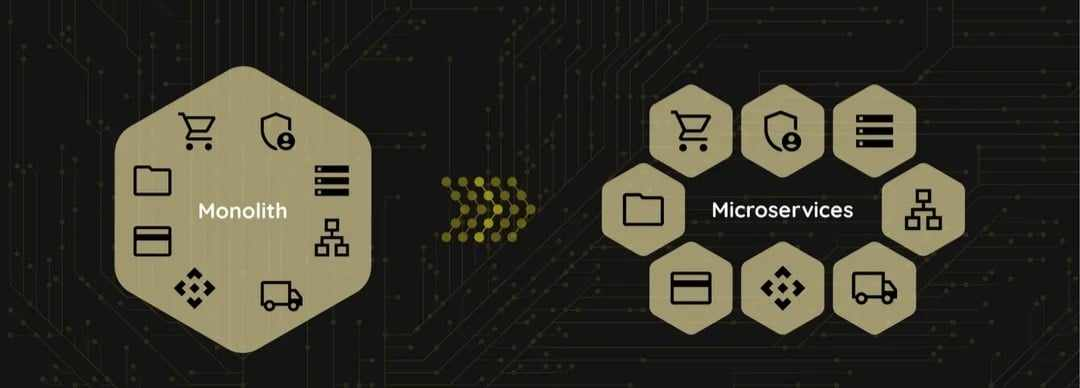
\includegraphics[height = 3cm]{pictures/ChuyenTu_KienTrucNguyenKhoi_Sang_KienTrucViDichVu.jpg}

% % \caption{ViDuHinhAnhTheoChieuDoc}

% \end{figure}

% \begin{figure}[h]

% \centering

% 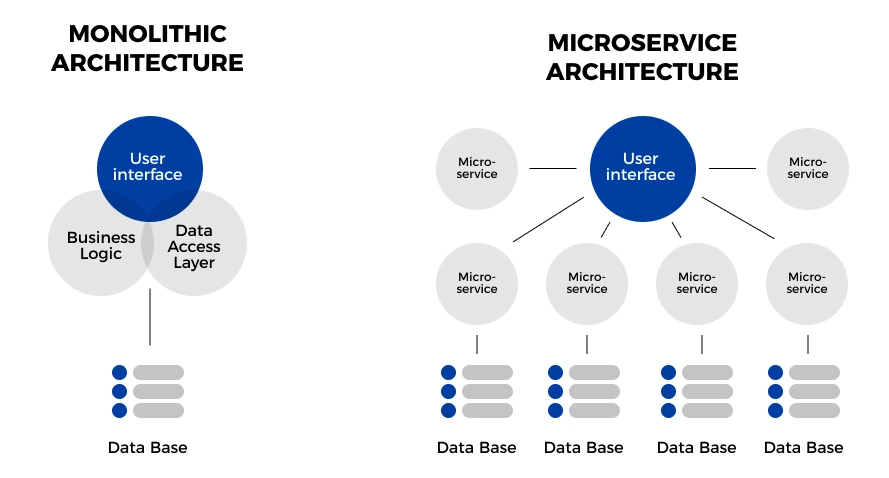
\includegraphics[height = 3cm]{pictures/AnhKhacNhau_KienTrucNguyenKhoi_KienTrucViDichVu.png}

% % \caption{ViDuHinhAnhTheoChieuDoc}

% \end{figure}

% Strangler Fig là chuyển mono sang dịch vụ



% \subsubsection{Một số đặc điểm và ưu điểm của kiến trúc vi dịch vụ}

% Kiến trúc vi dịch vụ có nhiều ưu điểm, đặc biệt với các dự án có quy mô lớn và phức tạp.

\begin{itemize}

    \item Kiến trúc vi dịch vụ phân chia dự án thành các dịch vụ nhỏ.

          \begin{itemize}

              \item Giúp việc phát triển và quản lý hệ thống dễ dàng hơn.

              \item Tận dụng sử dụng tài nguyên theo nhu cầu cho từng dịch vụ riêng.


          \end{itemize}
    \item Các dịch vụ độc lập về nghiệp vụ kinh doanh.
    
    Các nhóm không cần hiểu sâu về mọi khả năng kinh doanh.      Dẫn tới tốc độ phát triển thay đổi nhanh và   tốc độ định giá doanh nghiệp nhanh hơn.
    
    \item Các dịch vụ độc lập về         ngôn ngữ lập trình và CSDL
    \begin{itemize}

        \item     Kiến trúc vi dịch vụ sử dụng đa ngôn ngữ và công nghệ khác nhau. Từ đó tận dụng hiệu quả thế mạnh của từng ngôn ngữ, công nghệ phù hợp nhất cho yêu cầu nghiệp vụ cụ thể.   

        \item        Giảm chi phí và thời gian kiểm thử do ít ràng buộc.
        \item Ví dụ: Mỗi dịch vụ sử dụng ngôn ngữ lập trình nhau khác như: NodeJS, Go, Python, Java, CSharp,...
        
        
        
         
        \begin{figure}[h] 
        \centering
        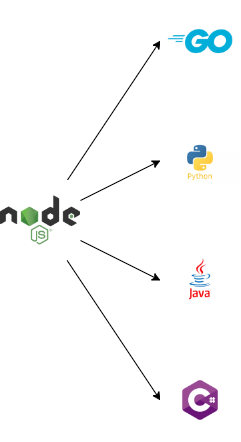
\includegraphics[height=3cm]{pictures/DaNgonNgu/_DaNgonNgu.png}
        \caption{ViDuHinhAnhTheoChieuDoc}  
        % % Thêm vào hình SQL riêng 
        \end{figure} 
        
       


        
        
        


    \end{itemize}
\end{itemize}

%     \item Các  
% 
%                         %     $VD: 




%                           \item Độc lập về     triển khai hệ thống



%                           Mỗi dịch vụ   triển khai độc lập và có thể thực hiện các thay đổi  mà không ảnh hưởng đến các dịch vụ khác.  





%           \end{itemize}
% \end{itemize}

% % Các dịch vụ ít phụ thuộc vào các dịch vụ khác.
% Giảm thiểu ràng buộc và tăng tính linh hoạt của hệ thống.
% Hệ thống có khả năng chịu lỗi cao tăng độ tin cậy.
% % Khả năng phục hồi : Kiến trúc phải được thiết kế để chịu đựng lỗi và các dịch vụ phải có khả năng xử lý lỗi một cách duyên dáng.
% Tính linh hoạt : Kiến trúc phải cho phép phát triển và triển khai nhanh chóng các dịch vụ mới cũng như khả năng thay đổi các dịch vụ hiện có một cách nhanh chóng và dễ dàng.
% \textbf{Từ đó    dễ dàng  mở rộng hệ thống.}
%%%%%%%%%%%%%%%%%%%%%%%%%%%%%%%%%%%%%



%%%%%%%%%%%%%%%%%%%%%%%%%%%%%%%%%%%%%


% Các dịch vụ tương tác với nhau qua hạ tầng mạng.

% Các dịch vụ tương tác với nhau qua hạ tầng mạng.

% Các dịch vụ tương tác với nhau qua hạ tầng mạng.

% Các dịch vụ tương tác với nhau qua hạ tầng mạng.

% Các dịch vụ tương tác với nhau qua hạ tầng mạng.

% Các dịch vụ tương tác với nhau qua hạ tầng mạng.

% Các dịch vụ tương tác với nhau qua hạ tầng mạng.

% Các dịch vụ tương tác với nhau qua hạ tầng mạng.

% Các dịch vụ tương tác với nhau qua hạ tầng mạng.

% \subsubsection{Một số nhược điểm và thách thức của kiến trúc vi dịch vụ}

% % Mặc dù kiến trúc vi dịch vụ có nhiều lợi ích nhưng  cũng có nhiều thách thức:

Chịu ảnh hưởng của đường truyền mạng.
Đồng bộ đồng hồ thời gian.
Ràng buộc về thứ tự sự kiện.
Tính nhất quán và toàn vẹn của dữ liệu.
Khả năng kiểm soát giao dịch.

Giám sát giữa các dịch vụ.
Bảo mật giao tiếp giữa các dịch vụ.


Phát hiện lỗi và sửa lỗi khó khăn, phức tạp hơn.




Chi phí xây dựng, quản lí vận hành lớn. 
 



% \subsubsection{Có thể thêm phần truyền thông trực tiếp, gián tiếp}

% \subsection{Giới thiệu về thiết kế hướng miền}

% Trong quá trình hoạt động kinh doanh, không phải mọi doanh nghiệp đều giữ nguyên mô hình kinh doanh được đưa ra ban đầu của mình. Khi quy mô thị trường thay đổi, việc chuyển đổi mô hình kinh doanh là điều cần thiết. Chuyển đổi kinh doanh như một công cụ linh hoạt giúp các doanh nghiệp có thể phát triển và tồn tại giữa các đối thủ của mình.

Ví dụ:






\begin{itemize}
    \item   Google bắt đầu như một công cụ tìm kiếm trực tuyến, nhưng sau đó đã mở rộng và thay đổi mô hình kinh doanh qua nhiều dịch vụ và sản phẩm khác nhau như: Dịch vụ đám mây Google Cloud Platform, thư điện tử Gmail, bản đồ Google Maps, lưu trữ tập tin Google Drive, \dots
    \item   Amazon từ hiệu sách trực tuyến đã trở thành thị trường cho nhà cung cấp khác như: Thương mại điện tử, Dịch vụ đám mây Amazon Web Services (AWS), \dots
\end{itemize}

\begin{figure}[h]

    \centering

    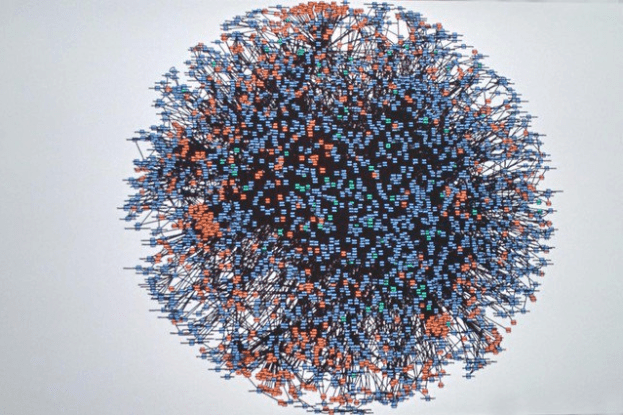
\includegraphics[width = 0.5\textwidth]{pictures/KienTrucViDichVuAmazon/main.png}

    \caption{Kiến trúc vi dịch vụ của Amazon}

\end{figure}


Đối với những doanh nghiệp không chuyển đổi kinh doanh sẽ không thể tồn tại.

Ví dụ: Gần đây, Baemin dịch vụ giao đồ ăn đã rời khỏi thị trường Việt Nam cũng do sức ép từ các đối thủ khác khiến Baemin khó cạnh tranh trong mảng kinh doanh cốt lõi là giao đồ ăn. Các đối thủ này không chỉ cung cấp dịch vụ giao đồ ăn mà còn có đặt xe, giao hàng,...


\begin{figure}[h]
    
    \centering
    
    % ![](pictures/Baemin.png)
    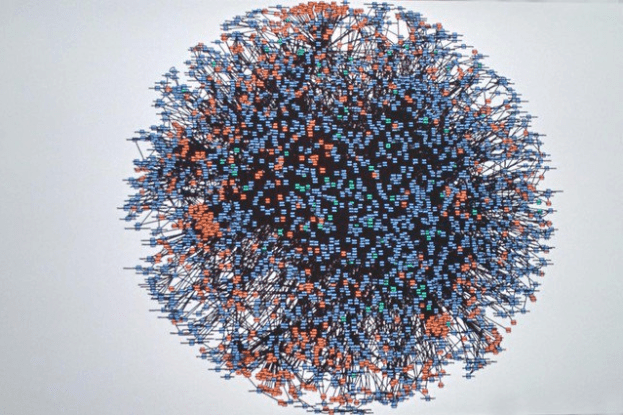
\includegraphics[width = 0.5\textwidth]{pictures/KienTrucViDichVuAmazon/main.png}

    \caption{  Baemin đã rời khỏi thị trường Việt Nam}

\end{figure}

%%%%%%%%%%%%%%%%%%%%%%%%%%%%%%%%%%%%%

% = > Hiện nay, các tổ chức doanh nghiệp có nhu cầu phát triển chuyển đổi kinh doanh để có thể tồn tại và phát triển khi thị trường thay đổi. Từ đó, đáp ứng nhu cầu của khách hàng, giúp mang đến ưu thế cạnh tranh so với các đối thủ. Do đó cần hệ thống chuyển đổi nhanh chóng đáp ứng nhu cầu của dự án và mong đợi của khách hàng.

% = > Kiến trúc vi dịch vụ giải quyết những thách thức và hỗ trợ doanh nghiệp chuyển đổi dễ dàng.

%%%%%%%%%%%%%%%%%%%%%%%%%%%%%%%%%%%%%

Tuy nhiên, để xây dựng được kiến trúc vi dịch vụ tốt cần phải tạo ra các dịch vụ nhỏ phù hợp và duy trì tính độc lập. Nếu không thực hiện đúng các nhóm phụ thuộc lẫn nhau và mất đi lợi thế của kiến trúc vi dịch vụ.

Và từ đó, mẫu thiết kế hướng miền sử dụng để phân tích xây dựng kiến trúc vi dịch vụ.

Thiết kế hướng miền xác định và tổ chức các dịch vụ dựa trên việc hiểu rõ về lĩnh vực kinh doanh, giúp dự án phản ánh đúng các quy trình và quy tắc kinh doanh.

%%%%%%%%%%%%%%%%%%%%%%%%%%%%%%%%%%%%%

% thiết kế hướng miền có thể trợ giúp như thế nào

% Thiết kế hướng miền (thiết kế hướng miền) có thể hỗ trợ kiến trúc và thiết kế kiến trúc vi dịch vụ theo nhiều cách:

% Bối cảnh giới hạn : thiết kế hướng miền nhấn mạnh việc xác định các bối cảnh giới hạn, là các khu vực riêng biệt của miền có ranh giới được xác định rõ ràng. Điều này có thể giúp xác định ranh giới của kiến trúc vi dịch vụ và đảm bảo rằng mỗi kiến trúc vi dịch vụ đều có trách nhiệm rõ ràng và tập trung.

% ngôn ngữ chung : thiết kế hướng miền khuyến khích sử dụng một ngôn ngữ chung được chia sẻ bởi cả chuyên gia ngành và nhân viên kỹ thuật. Điều này có thể giúp đảm bảo rằng các vi dịch vụ giao tiếp hiệu quả với nhau và phù hợp với yêu cầu kinh doanh.

% Ánh xạ bối cảnh: thiết kế hướng miền cung cấp các kỹ thuật để ánh xạ các mối quan hệ giữa các bối cảnh giới hạn. Điều này có thể giúp đảm bảo rằng các vi dịch vụ được thiết kế với sự hiểu biết rõ ràng về sự phụ thuộc của chúng vào các dịch vụ khác.

% Tập hợp: thiết kế hướng miền định nghĩa tập hợp là các cụm đối tượng liên quan cần được coi là một đơn vị nhất quán duy nhất. Điều này có thể giúp đảm bảo rằng các vi dịch vụ được thiết kế với sự hiểu biết rõ ràng về các yêu cầu về tính nhất quán của dữ liệu.

% Tương quan với bối cảnh giới hạn

% Mặc dù người ta thường khuyên nên căn chỉnh ranh giới của kiến trúc vi dịch vụ với ranh giới của bối cảnh giới hạn, nhưng điều đó không phải lúc nào cũng cần thiết hoặc khả thi. Một vi dịch vụ có thể gói gọn nhiều ngữ cảnh giới hạn hoặc một ngữ cảnh giới hạn có thể được phân chia thành nhiều vi dịch vụ, tùy thuộc vào nhu cầu cụ thể của hệ thống và sự cân bằng liên quan. Cuối cùng, mục tiêu là tạo ra một hệ thống mô - đun và có thể bảo trì, đáp ứng các yêu cầu kinh doanh và mối quan hệ giữa bối cảnh giới hạn và các vi dịch vụ phải được thiết kế phù hợp.

% Tương quan với API thực thể

% Nhìn chung, việc thiết kế các vi dịch vụ chỉ dựa trên các hoạt động CRUD của thực thể không được khuyến khích vì nó có thể dẫn đến một kiến trúc liên kết chặt chẽ và không hiệu quả. Các vi dịch vụ phải được thiết kế dựa trên khả năng kinh doanh, có thể phù hợp hoặc không phù hợp với hoạt động CRUD của thực thể.

% thiết kế hướng miền có thể giúp xác định các khả năng kinh doanh và xác định bối cảnh giới hạn, sau đó có thể được sử dụng để hướng dẫn thiết kế các vi dịch vụ. Bằng cách tập trung vào khả năng kinh doanh thay vì hoạt động CRUD thực thể, các vi dịch vụ có thể được liên kết lỏng lẻo hơn, mang tính mô - đun hơn, dễ dàng duy trì và phát triển hơn theo thời gian.



%%%%%%%%%%%
% \section{Yêu cầu nghiệp vụ}

% Yêu cầu nghiệp vụ xác định nội dung, phạm vi, mục tiêu và chức năng mong muốn của hệ thống.

% Nguồn: TCT: https://hoadondientu.gdt.gov.vn
% https://helpsme.misa.vn/2020/kb/quan - ly - hoa - don - dien - tu

% \subsection {Yêu cầu nghiệp vụ của bài toán phụ}

% Trang web "https: //hoadondientu.gdt.gov.vn" là trang web do Tổng Cục Thuế quản lý và sử dụng để thực hiện các quy trình liên quan đến thuế điện tử. Thực tế, yêu cầu đăng ký chính thức từ Tổng Cục Thuế dành cho cá nhân và doanh nghiệp. Vì em không có tài khoản chính thức nên ở đồ án này, em sẽ tạo  tong-cuc-thue-demo - một phiên bản giả lập của hệ thống chính thức, dành cho mục đích học tập phục vụ cho bài toán chính là "Xây dựng kiến trúc vi dịch vụ cho bài toán hóa đơn điện tử".


% \subsubsection{Các chức năng tổng quan của bài toán phụ}

% Để đơn giản hóa bài toán, các chức năng trong đồ án này đã thay đổi so với bài toán thực tế trong tài liệu hướng dẫn sử dụng cổng thông tin điện tử của TCT cho hóa đơn điện tử:

\textbf{Em đã bỏ qua hình thức hóa đơn}

Hóa đơn có mã của cơ quan thuế

Hóa đơn không có mã của cơ quan thuế

\textbf{Bỏ qua các loại hóa đơn khác nhau}

Hóa đơn điện tử giá trị gia tăng

Hóa đơn bán hàng

Hóa đơn bán tài sản công

Hóa đơn bán hàng dự trữ quốc gia

Hóa đơn khác

Phiếu xuất kho kiêm vận chuyển nội bộ

Phiếu xuất kho gửi bán hàng đại lý

\textbf{Bỏ qua phần ký số}

USB Token hay còn gọi là chữ ký số Token là một thiết bị mà mọi doanh nghiệp, tổ chức hiện nay đều cần phải có để thực hiện khai báo và nộp thuế điện tử, cũng như để giao dịch với khách hàng.

\textbf{Bỏ qua phần ký hiệu hóa đơn}

Vì mục đích của ký hiệu hóa đơn là nhóm 6 ký tự thể hiện thông tin về loại hóa đơn điện tử có mã hoặc không mã, năm lập hóa đơn, loại hóa đơn.

\textbf{Bỏ qua chức năng lập hóa đơn điều chỉnh}

E bỏ qua chức năng lập hóa đơn điều chỉnh và chỉ có chức năng lập hóa đơn thay thế.

\textbf{Bỏ qua chức năng phê duyệt hóa đơn}

\textbf{Bỏ qua định dạng file XML,PDF,HTML, EXCEL}

\textbf{Tóm lại, các chức năng tổng quan của tong - cuc - thue - demo bao gồm:}

\underline{\textsc{QUẢN LÝ TÀI KHOẢN}}

Đăng ký

% mail active

% active

Đăng nhập

Đăng xuất

Quên mật khẩu

% mail reset

% reset

Đổi mật khẩu

Thay đổi thông tin

\underline{\textsc{QUẢN LÝ HỆ THỐNG}}

Quản lý vai trò

Quản lý người dùng

\underline{\textsc{QUẢN LÝ DANH MỤC}}

Danh mục khách hàng

Danh mục hàng hóa

\underline{\textsc{QUẢN LÝ HÓA ĐƠN}}

Lập hóa đơn mới

Lập hóa đơn thay thế

Hủy hóa đơn

\underline{\textsc{TRA CỨU HÓA ĐƠN}}

Tra cứu hóa đơn khi NNT chưa đăng nhập

Tra cứu hóa đơn khi NNT đã đăng nhập

\underline{\textsc{GỬI PHẢN HỒI QUA THƯ ĐIỆN TỬ}}

Gửi thông tin của TCT đến NNT
% \subsection{Yêu cầu nghiệp vụ chưa xong}
% \subsection{Yêu cầu nghiệp vụ chưa xong}
% \subsection{Yêu cầu nghiệp vụ chưa xong}
% \subsection{Yêu cầu nghiệp vụ chưa xong}
% \subsection{Yêu cầu nghiệp vụ chưa xong}
% chưa xong

% %@ %@ %@ %@ %@ %@ Mẫu mail

%!<! - - // NNT nhận được thư điện tử của CQT thông báo tiếp nhận tờ khai đăng ký - - >

Trong thời gian 15 phút kể từ khi nhận được tờ khai đăng ký của NNT, Cổng điện tử gửi thư điện tử thông báo về việc tiếp nhận/không tiếp nhận tờ khai đăng ký của NNT.

Nội dung mẫu:

```
Tiêu đề: (TCT Demo) Thông báo về việc tiếp nhận tờ khai đăng ký sử dụng hóa đơn điện tử
Kính gửi: {{Tên NNT}}
Mã số thuế: {{Mã số thuế}}

Căn cứ Tờ khai đăng ký sử dụng hóa đơn điện tử - Ban hành kèm theo Nghị định số 123/2020/NĐ - CP của người nộp thuế (NNT) gửi tới cơ quan thuế ngày {{Ngày nhận}}, cơ quan thuế tiếp nhận Tờ khai đăng ký sử dụng hóa đơn điện tử của NNT, cụ thể như sau:
Tên tờ khai: Tờ khai đăng ký sử dụng hóa đơn điện tử
Mã giao dịch điện tử: {{Mã số thuế + Thời gian}}

Cơ quan thuế thông báo để NNT được biết và thực hiện.
```

%!<! - - NNT nhận được thư điện tử của CQT chấp nhận/không chấp nhận đăng ký sử dụng HĐĐT - - >

Trong thời gian 01 ngày làm việc kể từ ngày Cổng điện tử gửi thông báo về việc tiếp nhận, cơ quan thuế quản lý sẽ gửi thông báo về việc chấp nhận/không chấp nhận đăng ký sử dụng hóa đơn điện tử.

Nội dung mẫu chấp nhận đăng ký sử dụng HĐĐT:

```
Tiêu đề: (TCT Demo) Thông báo về việc chấp nhận đăng ký sử dụng hóa đơn điện tử
Kính gửi: {{Tên NNT}}
Mã số thuế: {{Mã số thuế}}

Sau khi xem xét tờ khai đăng ký sử dụng hóa đơn điện tử của NNT gửi đến cơ quan thuế ngày {{Ngày nhận}}.
Cơ quan thuế thông báo chấp nhận đề nghị đăng ký sử dụng hóa đơn điện tử của NNT.

Cơ quan thuế thông báo để NNT được biết và thực hiện.
```

Nội dung mẫu không chấp nhận đăng ký sử dụng HĐĐT:

```
Tiêu đề: (TCT Demo) Thông báo về việc không chấp nhận đăng ký sử dụng hóa đơn điện tử
Kính gửi: {{Tên NNT}}
Mã số thuế: {{Mã số thuế}}

Sau khi xem xét tờ khai đăng ký sử dụng hóa đơn điện tử của NNT gửi đến cơ quan thuế ngày {{Ngày nhận}}.
Cơ quan thuế thông báo không chấp nhận đề nghị đăng ký sử dụng hóa đơn điện tử của NNT.

Cơ quan thuế thông báo để NNT được biết và thực hiện.
```

%!<! - - NNT nhận được Thông báo tài khoản sử dụng tra cứu HĐĐT trên cổng thông tin điện tử của TCT - - >

Sau khi NNT nhận được thông báo về việc chấp nhận đăng ký sử dụng hóa đơn điện tử, cơ quan thuế gửi thông báo tài khoản sử dụng của NNT qua thư điện tử bao gồm Tên tài khoản và Mật khẩu.

Nội dung mẫu:

```
Tiêu đề: (TCT Demo) Thông báo tài khoản sử dụng tra cứu HĐĐT trên cổng thông tin điện tử của TCT
Kính gửi: {{Tên NNT}}
Mã số thuế: {{Mã số thuế}}

Sau khi xem xét tờ khai đăng ký sử dụng hóa đơn điện tử cơ quan thuế tiếp nhận ngày {{Ngày nhận}}.
Cơ quan thuế thông báo chấp nhận đề nghị đăng ký sử dụng hóa đơn điện tử của NNT và gửi thông tin tài khoản sử dụng tra cứu HĐĐT trên cổng thông tin điện tử của TCT như sau:
Tên tài khoản: {{admin + Mã số thuế}}
Mật khẩu: {{Mật khẩu}}

Cơ quan thuế thông báo để NNT được biết và thực hiện.
```

%!<! - - - - >
%!<! - - - - >
%!<! - - - - >
%!<! - - - - >
%!<! - - - - >
%!<! - - - - >
%!<! - - - - >
%!<! - - - - >
%!<! - - - - >
%!<! - - - - >

%!<! - - NNT nhận được thư điện tử của CQT thông báo tiếp nhận tờ khai đăng ký thay đổi - - >

Trong thời gian 15 phút kể từ khi nhận được tờ khai đăng ký của NNT, Cổng điện tử gửi thư điện tử thông báo về việc tiếp nhận/không tiếp nhận tờ khai đăng ký thay đổi thông tin đăng ký sử dụng của NNT.

Nội dung mẫu:

```
Tiêu đề: (TCT Demo) Thông báo về việc tiếp nhận tờ khai đăng ký thay đổi thông tin đăng ký sử dụng của NNT
Kính gửi: {{Tên NNT}}
Mã số thuế: {{Mã số thuế}}

Căn cứ Tờ khai đăng ký thay đổi thông tin đăng ký sử dụng của NNT gửi tới cơ quan thuế ngày {{Ngày nhận}}, cơ quan thuế tiếp nhận Tờ khai đăng ký sử dụng hóa đơn điện tử của NNT, cụ thể như sau:
Tên tờ khai: Tờ khai đăng ký thay đổi thông tin đăng ký sử dụng của NNT
Mã giao dịch điện tử: {{Mã số thuế + Thời gian}}

Cơ quan thuế thông báo để NNT được biết và thực hiện.
```

%!<! - - NNT nhận được thư điện tử của CQT chấp nhận/không chấp nhận đăng ký sử dụng HĐĐT - - >

Trong thời gian 01 ngày làm việc kể từ ngày Cổng điện tử gửi thông báo về việc tiếp nhận, cơ quan thuế quản lý sẽ gửi thông báo về việc chấp nhận/không chấp nhận đăng ký thay đổi thông tin đăng ký sử dụng của NNT.

Nội dung mẫu chấp nhận đăng ký thay đổi thông tin đăng ký sử dụng của NNT

```
Tiêu đề: (TCT Demo) Thông báo về việc chấp nhận đăng ký thay đổi thông tin đăng ký sử dụng của NNT
Kính gửi: {{Tên NNT}}
Mã số thuế: {{Mã số thuế}}

Sau khi xem xét tờ khai đăng ký thay đổi thông tin đăng ký sử dụng của NNT gửi đến cơ quan thuế ngày {{Ngày nhận}}.
Cơ quan thuế thông báo chấp nhận đề nghị đăng ký thay đổi thông tin đăng ký sử dụng của NNT.

Cơ quan thuế thông báo để NNT được biết và thực hiện.
```

Nội dung mẫu không chấp nhận đăng ký thay đổi thông tin đăng ký sử dụng của NNT

```
Tiêu đề: (TCT Demo) Thông báo về việc không chấp nhận đăng ký thay đổi thông tin đăng ký sử dụng của NNT
Kính gửi: {{Tên NNT}}
Mã số thuế: {{Mã số thuế}}

Sau khi xem xét tờ khai đăng ký thay đổi thông tin đăng ký sử dụng của NNT gửi đến cơ quan thuế ngày {{Ngày nhận}}.
Cơ quan thuế thông báo không chấp nhận đề nghị đăng ký thay đổi thông tin đăng ký sử dụng của NNT.

Cơ quan thuế thông báo để NNT được biết và thực hiện.
```

%!<! - - - - >
%!<! - - - - >
%!<! - - - - >
%!<! - - - - >
%!<! - - - - >
%!<! - - - - >
%!<! - - - - >

%!<! - - Sau khi gửi yêu cầu lấy lại mật khẩu NNT sẽ nhận được thông báo của CQT qua gửi thư điện tử - - >

Nội dung mẫu:

```
Tiêu đề: (TCT Demo) Thông báo về việc lấy lại mật khẩu
Kính gửi: {{Tên NNT}}
Mã số thuế: {{Mã số thuế}}

Sau khi xem xét yêu cầu lấy lại mật khẩu của NNT gửi đến cơ quan thuế ngày {{Ngày nhận}}.
Cơ quan thuế gửi thông tin tài khoản sử dụng tra cứu HĐĐT trên cổng thông tin điện tử của TCT như sau:
Tên tài khoản: {{Tên tài khoản}}
Mật khẩu mới: {{Mật khẩu mới}}

Cơ quan thuế thông báo để NNT được biết và thực hiện.
```

%@ %@ %@ Chi tiết các chức năng của TCT Demo:

Chi tiết các chức năng của TCT Demo:

QUẢN LÝ TÀI KHOẢN

Quản lý tài khoản là một chức năng phổ biến trong nhiều ứng dụng. Chức năng này đảm bảo tính bảo mật và an toàn trong việc sử dụng tài khoản.

%!<! - - Chức năng: "Đăng ký sử dụng hóa đơn điện tử" - - >

NNT nhập MST có 10 ký tự cho cá nhân, doanh nghiệp hoặc 14 ký tự cho chi nhánh của doanh nghiệp với định dạng "Mã số thuế doanh nghiệp - Mã chi nhánh".
Ví dụ:
Mã số thuế 10 ký tự: 0123456789
Mã số thuế 14 ký tự: 0123456789 - 001

Hệ thống tự động hiển thị thông tin Đăng ký thuế của NNT bao gồm "Tên của NNT", "Mã cơ quan thuế quản lý" và "Tên cơ quan thuế quản lý".

Tiếp theo, NNT nhập các thông tin hợp lệ: "Người liên hệ", "Điện thoại liên hệ", "Địa chỉ liên hệ", "Thư điện tử".

Cuối cùng, NNT gửi đăng ký với thông tin "Ngày thực hiện" là ngày NNT đang đăng ký hóa đơn điện tử.

Sau khi gửi thông tin đăng kí NNT sẽ nhận được thông báo làm việc của CQT qua gửi thư điện tử về việc tiếp nhận và chấp nhận đăng ký, cùng với tài khoản và mật khẩu cho NNT.

%!<! - - // Nếu mã số thuế không đúng định dạng, hệ thống sẽ thông báo: "Mã số thuế phải có độ dài 10 hoặc 14 ký tự và đúng định dạng". - - >
%!<! - - // Nếu mã số thuế tồn tại, hệ thống kiểm tra xem NNT đã đăng ký sử dụng hóa đơn điện tử khác chưa. Nếu đã tồn tại tờ khai đăng ký, hệ thống thông báo: "Đã tồn tại tờ khai đăng ký sử dụng hóa đơn điện tử khác của NNT đã được cơ quan thuế chấp nhận". - - >

%!<! - - // Người liên hệ: phải chứa một chuỗi kí tự và không được để trống. - - >
%!<! - - // Điện thoại liên hệ: phải chứa một chuỗi kí tự số và dấu " + " ở đầu chuỗi (nếu có) và không được để trống. - - >
%!<! - - // Địa chỉ liên hệ: phải chứa một chuỗi kí tự và không được để trống. - - >
%!<! - - // Thư điện tử: phải chứa một chuỗi kí tự có định dạng email và không được để trống. - - >

%!<! - - // Khi NNT nhấn nút "Ký gửi", hệ thống sẽ hiển thị thông báo hỏi "Xác nhận ký gửi" với hai lựa chọn là "Đồng ý" hoặc "Hủy bỏ". - - >
%!<! - - // Nếu NNT chọn "Đồng ý", hệ thống sẽ thông báo: "Gửi thông tin đăng ký sử dụng hóa đơn điện tử cho cơ quan thuế thành công". - - >

%!<! - - - - >
%!<! - - Chức năng: "Thay đổi đăng ký sử dụng hóa đơn điện tử" - - >

Trong quá trình sử dụng hóa đơn điện tử, khi NNT muốn thay đổi đăng ký sử dụng hóa đơn, họ có thể sử dụng chức năng "Thay đổi đăng ký sử dụng hóa đơn điện tử".

NNT Nhập thông tin có thể thay đổi, bao gồm: Tên NNT, Người liên hệ, Điện thoại liên hệ, Địa chỉ liên hệ, Thư điện tử.
Cuối cùng, NNT gửi đăng ký thay đổi với thông tin "Ngày thực hiện" là ngày NNT đang đăng ký thay đổi hóa đơn điện tử.

Sau khi gửi thông tin thay đổi đăng ký, NNT sẽ nhận được thông báo làm việc từ cơ quan thuế qua thư điện tử về việc tiếp nhận và chấp nhận thay đổi đăng ký cho NNT.

%!<! - - Chức năng: "Đăng nhập tài khoản" - - >

Sau khi CQT gửi thư điện tử chứa tài khoản và mật khẩu cho NNT, NNT thực hiện nhập đầy đủ thông tin bao gồm: Tên đăng nhập, Mật khẩu để thực hiện việc đăng nhập vào tài khoản.

%!<! - - Chức năng: "Đăng xuất tài khoản" - - >

Chức năng để NNT đăng xuất tài khoản.

%!<! - - Chức năng: "Đổi mật khẩu" - - >

NNT cung cấp đầy đủ thông tin bao gồm: Mật khẩu cũ, Mật khẩu mới và Nhập lại mật khẩu mới để thực hiện việc thay đổi mật khẩu.

%!<! - - Chức năng: "Quên mật khẩu" - - >

NNT cung cấp đầy đủ thông tin bao gồm: Tên đăng nhập, Thư điện tử. Sau đó, nhấn "Quên mật khẩu" để khôi phục mật khẩu. CQT gửi mật khẩu mới về email của NNT.

%!<! - - QUẢN LÝ HỆ THỐNG - - >

%!<! - - Chức năng: "Quản lý vai trò" - - >

Người quản trị hệ thống (admin) là một vai trò cố định được phép sử dụng tất cả các chức năng trên Cổng điện tử.
Người quản trị hệ thống có thể thực hiện CRUD "Vai trò" với các thông tin bao gồm: "ID", "Tên vai trò" và "Quyền".

Các quyền bao gồm:
Thay đổi đăng ký sử dụng hóa đơn điện tử
Quản lý vai trò
Quản lý người dùng
Quản lí danh mục
Quản lí hóa đơn
Tra cứu hóa đơn

%!<! - - Chức năng: "Quản lý người dùng" - - >

Người quản trị hệ thống có thể thực hiện CRUD "Người dùng" với các thông tin bao gồm: "Tên người dùng", "Mật khẩu", "Điện thoại", "Thư điện tử" và "Vai trò".

%!<! - - QUẢN LÝ DANH MỤC - - >

%!<! - - Chức năng: "Danh mục khách hàng" - - >

Chức năng này thực hiện CRUD "Khách hàng" có các thông tin: "Mã khách hàng", "Tên khách hàng", "Mã số thuế", "Tên NNT", "Địa chỉ", "SĐT khách hàng", Số tài khoản, Ngân hàng

%!<! - - Chức năng: "Danh mục hàng hóa" - - >

Chức năng này thực hiện CRUD "Hàng hóa" có các thông tin: "Mã hàng hóa, dịch vụ", "Tên hàng hóa, dịch vụ", "Đơn vị tính", "Đơn giá", "Thuế suất".

%!<! - - QUẢN LÝ HÓA ĐƠN ĐIỆN TỬ - - >

%!<! - - Chức năng: "Lập hóa đơn mới" - - >

Nhập thông tin người bán: MST người bán, Tên người bán, Địa chỉ người bán, Số điện thoại người bán.

Nhập thông tin người mua: Mã khách hàng, Tên khách hàng, Mã số thuế, Địa chỉ khách hàng, SĐT khách hàng.

Nhập thông tin hàng hóa, dịch vụ: "Số thứ tự", "Mã hàng hóa, dịch vụ", "Tên hàng hóa, dịch vụ", "Đơn vị tính", "Đơn giá", "Thuế suất" và "Số lượng".

Hệ thống tự động tính toán:

- Ngày lập hóa đơn sẽ tự động là ngày hiện tại khi người lập tạo hóa đơn mới.

- Tổng tiền trước thuế.

- Tổng tiền sau thuế.

%!<! - - Chức năng: "Lập hóa đơn thay thế" - - >

Chức năng này cho phép thay đổi các thông tin trong hóa đơn gốc.

Lưu ý:

- Hãy lưu trữ thông tin ID của hóa đơn thay thế trong trạng thái "Bị thay thế" của hóa đơn gốc.

- Hãy lưu trữ thông tin ID của hóa đơn gốc trong trạng thái "Thay thế" của hóa đơn thay thế.

%!<! - - Chức năng: "Hủy hóa đơn" - - >

Chức năng này cho phép xóa hóa đơn và các hóa đơn thay thế liên quan.

%!<! - - TRA CỨU HÓA ĐƠN - - >

Người sử dụng có thể thực hiện tra cứu hóa đơn trên cổng thông tin điện tử theo 2 cách:
Cách 1: Tra cứu hóa đơn khi NNT chưa đăng nhập
Cách 2: Tra cứu hóa đơn khi NNT đã đăng nhập

%!<! - - Chức năng: "Tra cứu hóa đơn khi NNT chưa đăng nhập" - - >

%!<! - - Tra cứu thông tin hóa đơn - - >

Người tra cứu nhập thông tin bao gồm: Mã số thuế người bán, Số hóa đơn, Tổng tiền thuế, Tổng tiền thanh toán, Ngày lập hóa đơn.

%!<! - - Kết quả: - - >
%!<! - - - Nếu hóa đơn điện tử không hợp lệ, hệ thống sẽ hiển thị thông báo: "Không tồn tại hóa đơn có thông tin trùng khớp với các thông tin tổ chức, cá nhân tìm kiếm”. - - >
%!<! - - - Nếu hóa đơn điện tử hợp lệ, hệ thống sẽ hiển thị thông báo: "Tồn tại hóa đơn có thông tin trùng khớp với các thông tin tổ chức, cá nhân tìm kiếm". - - >
%!<! - - - Nếu hóa đơn tìm kiếm là hóa đơn thay thế, bị thay thế hệ thống sẽ hiển thị thông tin bổ sung về hóa đơn liên quan: "Hóa đơn này là hóa đơn thay thế cho hóa đơn có ID: {{ID}}" hoặc "Hóa đơn này là hóa đơn bị thay thế của hóa đơn có ID: {{ID}}". - - >

%!<! - - Tra cứu thông tin "Mã số thuế" - - >

Người tra cứu nhập thông tin bao gồm: Mã số thuế.

%!<! - - Kết quả: - - >
%!<! - - - Nếu đã đăng kí, hệ thống sẽ hiển thị thông báo: “MST 0107001729 đã đăng ký sử dụng hóa đơn điện tử theo Nghị định 123/2020/NĐ - CP". - - >
%!<! - - - Nếu NNT chưa đăng kí hoặc đã đăng kí nhưng cơ quan thuế có thông báo về việc không được chấp nhận đăng kí sử dụng hóa đơn điện tử, hệ thống sẽ hiển thị thông báo: “MST 0107001728 chưa sử dụng hóa đơn điện tử theo Nghị định 123/2020/NĐ - CP". - - >
%!<! - - Chức năng: "Tra cứu hóa đơn khi NNT đã đăng nhập" - - >

Cổng điện tử hỗ trợ tra cứu 2 loại hóa đơn là hóa đơn bán ra và hóa đơn mua vào.

Người tra cứu nhập thông tin tra cứu bao gồm: Mã số thuế người bán, Ngày lập hóa đơn và Số hóa đơn.

Cổng điện tử hỗ trợ các chức năng sau: Xem thông tin hóa đơn, In hóa đơn và Xuất hóa đơn (định dạng Excel, XML, PDF).

%!<! - - GỬI PHẢN HỒI QUA THƯ ĐIỆN TỬ - - >

%!<! - - - Gửi thông tin làm việc của TCT cho yêu cầu của NNT - - >

%!<! - - $ NNT nhận được thư điện tử của CQT thông báo tiếp nhận tờ khai đăng ký - - >

%!<! - - $ NNT nhận được thư điện tử của CQT chấp nhận/không chấp nhận đăng ký sử dụng HĐĐT - - >

%!<! - - $ NNT nhận được Thông báo tài khoản sử dụng tra cứu HĐĐT trên cổng thông tin điện tử của TCT - - >

%!<! - - $ NNT nhận được thư điện tử của CQT thông báo tiếp nhận tờ khai đăng ký thay đổi - - >

%!<! - - $ NNT nhận được thư điện tử của CQT chấp nhận/không chấp nhận đăng ký sử dụng HĐĐT - - >
%!<! - - Yêu cầu nghiệp vụ của bài toán chính - - >

%!<! - - Các chức năng của bài toán chính - - >

%!<! - - THÔNG BÁO - - >

Chức năng CRUD "Thông báo" bao gồm các thông tin: ID, tiêu đề, nội dung, thời gian.

%!<! - - QUẢN LÝ TÀI KHOẢN - - >

Tương tự " TCT Demo" với các chức năng sau:

Đăng ký
Đăng nhập
Đăng xuất
Quên mật khẩu
Xem thông tin
Thay đổi thông tin
Đổi mật khẩu

%!<! - - CẤU HÌNH EMAIL - - >

Cấu hình bao gồm:

Địa chỉ email
Mật khẩu email

Loại email gửi:

Xác nhận tài khoản mới
Quên mật khẩu
Gửi thông tin hóa đơn cho khách hàng

%!<! - - QUẢN LÝ DANH MỤC - - >

Tương tự " TCT Demo" bao gồm:

Danh mục khách hàng
Danh mục hàng hóa

%!<! - - QUẢN LÝ HỆ THỐNG - - >

Tương tự " TCT Demo" nhưng có thêm quyền "Cấu hình Email".

%!<! - - QUẢN LÝ HÓA ĐƠN ĐIỆN TỬ - - >

Tương tự " TCT Demo"

%!<! - - TRA CỨU HÓA ĐƠN - - >

Có 3 cách tra cứu:

Tra cứu 1 hóa đơn theo "Mã hóa đơn"
Tra cứu tất cả hóa đơn bán ra
Tra cứu tất cả hóa đơn mua vào

%!<! - - BÁO CÁO VÀ PHÂN TÍCH HÓA ĐƠN - - >

Các chức năng bao gồm:

Số lượng hóa đơn đã sử dụng
Tổng tiền trước thuế
Tổng tiền sau thuế
Tổng số tiền thuế
Số lượng khách hàng
Số lượng sản phẩm

%@ %@ %@ Tự động

Nghiệp vụ của bài toán chính
Các chức năng của bài toán chính
THÔNG BÁO
CRUD thông báo có (id, tiêu đề, nội dung, thời gian)
TÀI KHOẢN
Sử dụng tài khoản của " TCT Demo" với các chức năng tương tự Đăng ký, Đăng nhập, Đăng xuất, Quên mật khẩu, Xem thông tin, Thay đổi thông tin, Đổi mật khẩu
CẤU HÌNH EMAIL ĐỂ GỬI HÓA ĐƠN CHO KHÁCH HÀNG

Địa chỉ email
Mật khẩu email
CHỨC NĂNG DANH MỤC
Giống với " TCT Demo" gồm "Danh mục khách hàng" và "Danh mục hàng hóa"
TRA CỨU HÓA ĐƠN:
Có 3 cách tra cứu:
Tra cứu 1 hóa đơn theo "Mã hóa đơn".
Tra cứu tất cả hóa đơn bán ra.
Tra cứu tất cả hóa đơn mua vào.
BÁO CÁO VÀ PHÂN TÍCH HÓA ĐƠN

Số lượng hóa đơn đã sử dụng
Tổng trước thuế
Tổng sau thuế
Tổng số tiền thuế
Số lượng khách hàng
Số lượng sản phẩm

%!<! - - - - >
%!<! - - Phân quyền - - >
%!<! - - Thay đổi - - >
%!<! - - Lập hóa đơn mới - - >
%!<! - - Tra cứu - - >
%!<! - - mail - - >

%@ %@ %@ 4. Các sơ đồ phân tích thiết kế hệ thống

%@ %@ %@ %@ %@ %@ 4.1. UML Use Case Diagrams

%@ %@ %@ %@ %@ %@ 4.2. UML Activity Diagrams

%@ %@ %@ %@ %@ %@ 4.3. UML Sequence Diagrams

%@ %@ %@ %@ %@ %@ 4.4. UML Class Diagrams


%%%%%%%%%%%
% \section{Chi tiết và áp dụng thiết kế hướng miền}
% https:// thiết kế hướng miền - practitioners.com/home/glossary
% https: //www.infoq.com/minibooks/domain - driven - design - quickly

% \subsection{Đôi nét về thiết kế hướng miền (DomainDrivenDesign)}

% % Thiết kế hướng miền được Eric Evans giới thiệu trong cuốn sách "DomainDrivenDesign: Tackling Complexity in the Heart of Software".

Thiết kế hướng miền (DomainDrivenDesign) là một phương pháp thiết kế phần mềm tập trung vào việc hiểu rõ và mô hình hóa lĩnh vực kinh doanh của một tổ chức.

Thiết kế hướng miền nhấn mạnh việc sử dụng lĩnh vực nghiệp vụ kinh doanh để thảo luận và đề xuất giải pháp đáp ứng nhu cầu. Vì để tạo một phần mềm tốt, chúng ta cần phải hiểu rõ về chính phần mềm đó. Chính vì vậy để đạt được kết quả như mong đợi, chúng ta thường bắt đầu từ yêu cầu nghiệp vụ.

Trong nhiều ứng dụng thường có phần xử lý các công việc không liên quan đến vấn đề nghiệp vụ như truy cập file, hạ tầng mạng, CSDL,... trong đối tượng nghiệp vụ kinh doanh. Cách này giúp tốc độ hoàn thiện ứng dụng nhanh. Tuy nhiên, cách này làm cho thiết kế bị mất đi tính hướng đối tượng trong thực tế với mức độ doanh nghiệp lớn. Đây là lý do thiết kế hướng miền trở nên quan trọng.

Trong kiến trúc vi dịch vụ, thiết kế hướng miền giúp đảm bảo rằng mỗi dịch vụ được thiết kế phản ánh một phần cụ thể của lĩnh vực kinh doanh. Mỗi dịch vụ được quản lí bởi một nhóm nhỏ được hỗ trợ bởi các chuyên gia ngành.

% %!<! - - Domain - Driven Design : https:// thiết kế hướng miền - practitioners.com/domain - driven - design - - >

% thường được sử dụng trong các dự án phần mềm phức tạp, quy mô lớn trong đó lĩnh vực kinh doanh có tính đặc thù cao và phần mềm phải phản ánh chính xác các quy trình kinh doanh cơ bản.



% \subsection{Miền (Domain)}

% Phần mềm được tạo ra để xử lý sự phức tạp trong cuộc sống hiện đại. Việc phát triển phần mềm liên kết chặt chẽ với một số khía cạnh cụ thể trong cuộc sống của chúng ta.

Miền (Domain) đề cập đến phạm vi kiến thức và vấn đề mà hệ thống hoặc dự án cụ thể đang xử lý.

Về góc độ kinh doanh: miền đại diện cho một lĩnh vực hoặc ngành mà doanh nghiệp hoạt động.
Về góc độ phần mềm: miền có thể coi là đại diện cho không gian vấn đề của phần mềm đó.

Phần mềm cần phản ánh đúng miền và hiện thực hóa chính xác miền.

%!<! - - $VD: Ở đồ án này, miền được xác định là bài toán giải pháp hóa đơn điện tử. - - >

% %!<! - - Domain : https:// thiết kế hướng miền - practitioners.com/domain - - >
% %!<! - - Domain : https:// thiết kế hướng miền - practitioners.com/domain - - >
% %!<! - - Domain : https:// thiết kế hướng miền - practitioners.com/domain - - >
% %!<! - - Domain : https:// thiết kế hướng miền - practitioners.com/domain - - >
% %!<! - - Domain : https:// thiết kế hướng miền - practitioners.com/domain - - >
% %!<! - - Domain : https:// thiết kế hướng miền - practitioners.com/domain - - >
% %!<! - - Domain : https:// thiết kế hướng miền - practitioners.com/domain - - >
% %!<! - - Domain : https:// thiết kế hướng miền - practitioners.com/domain - - >

%!<! - - [[Domain]] A sphere of knowledge, influence, or activity. - - >

Trang chủTrang chủBảng chú giảiLãnh địa
Lãnh địa
Trong thiết kế hướng miền (thiết kế hướng miền), miền là một phạm vi kiến thức, ảnh hưởng hoặc hoạt động đại diện cho một lĩnh vực chuyên môn hoặc mối quan tâm cụ thể. Miền là không gian vấn đề mà phần mềm đang được xây dựng để giải quyết và nó thể hiện vấn đề hoặc cơ hội kinh doanh mà phần mềm có nhiệm vụ giải quyết.

Miền có thể là một ngành cụ thể, chẳng hạn như chăm sóc sức khỏe, tài chính hoặc thương mại điện tử hoặc có thể là một lĩnh vực quan tâm cụ thể trong một ngành, chẳng hạn như quản lý hàng tồn kho, quản lý khách hàng hoặc hậu cần.

Trong thiết kế hướng miền, mục tiêu là tạo ra một mô hình miền thể hiện chính xác các khái niệm và mối quan hệ trong thế giới thực trong miền và sử dụng mô hình này làm cơ sở cho việc thiết kế và phát triển phần mềm. Mô hình miền này phải phản ánh miền kinh doanh, nó phải dễ hiểu đối với các chuyên gia miền, nhà phát triển và các bên liên quan và nó phải là xương sống của hệ thống phần mềm.

Một miền có thể được xác định bởi các quy tắc kinh doanh, quy trình kinh doanh, các thực thể kinh doanh và các mối quan hệ của chúng, các yêu cầu kinh doanh và mục tiêu kinh doanh.

Miền là trái tim của thiết kế hướng miền, là nền tảng của phần mềm và là điểm khởi đầu của quá trình phát triển. Hiểu miền là rất quan trọng để có thể tạo ra một phần mềm phù hợp với nhu cầu kinh doanh, ít phức tạp hơn, dễ bảo trì hơn và dễ thích ứng hơn với thay đổi.

Xem thêm	 Miền phụ, miền vấn đề, miền giải pháp, bối cảnh giới hạn



% \subsection{Chuyên gia ngành}

% An incisive expression of the primary concerns of the chuyên gia ngành s and their most relevant knowledge. A deep model sloughs off superficial aspects of the domain and naive interpretations.
%!<! - - [[Domain Expert]] A member of a software project whose field is the domain of the application, rather than software development. Not just any user of the software, the chuyên gia ngành has deep knowledge of the subject. - - >
% https:// thiết kế hướng miền - practitioners.com/home/glossary/domain - expert
% https:// thiết kế hướng miền - practitioners.com/home/glossary/domain - expert
% https:// thiết kế hướng miền - practitioners.com/home/glossary/domain - expert
% https:// thiết kế hướng miền - practitioners.com/home/glossary/domain - expert
% https:// thiết kế hướng miền - practitioners.com/home/glossary/domain - expert
% https:// thiết kế hướng miền - practitioners.com/home/glossary/domain - expert
% https:// thiết kế hướng miền - practitioners.com/home/glossary/domain - expert
% https:// thiết kế hướng miền - practitioners.com/home/glossary/domain - expert
% https:// thiết kế hướng miền - practitioners.com/home/glossary/domain - expert
% https:// thiết kế hướng miền - practitioners.com/home/glossary/domain - expert

Trang chủTrang chủBảng chú giải Chuyên gia ngành
Chuyên gia ngành
Trong Thiết kế hướng miền (thiết kế hướng miền), chuyên gia ngành là người có kiến thức và hiểu biết sâu sắc về miền kinh doanh hoặc lĩnh vực vấn đề đang được hệ thống phần mềm giải quyết. Chuyên gia ngành có kiến thức chuyên môn về các quy tắc, quy trình và khái niệm kinh doanh liên quan đến hệ thống đang được xây dựng và đóng vai trò là nguồn thông tin chính cho nhóm phát triển. Chuyên gia ngành giúp đảm bảo rằng mô hình miền thể hiện chính xác miền doanh nghiệp và hệ thống đang được xây dựng giải quyết đúng vấn đề cũng như giải quyết đúng nhu cầu kinh doanh.



% \subsection{Miền phụ (Sub - Domain)}

% Miền được tạo thành từ nhiều miền phụ.

Ví dụ: Trong miền thương mại điện tử lớn. Có thể có một số miền phụ:

\begin{itemize}

\item Miền phụ quản lý hàng tồn kho: liên quan đến việc quản lý sản phẩm trong kho hàng.

\item Miền phụ quản lý khách hàng: liên quan đến việc quản lý tài khoản khách hàng.

\item Miền phụ vận chuyển: liên quan đến việc quản lý việc vận chuyển giao hàng.

\end{itemize}

Trong một miền phức tạp, không thể có một chuyên gia ngành có kiến thức về tất cả các miền phụ.

Có ba loại miền phụ: 
\begin{itemize}
    
    \item     Miền phụ chung (Generic Subdomain) 
\item     Miền phụ cốt lõi (Core Subdomain) 
\item     Miền phụ hỗ trợ (Supporting Subdomain) 

\end{itemize} 





\end{document}


\subsubsection{xxxxxxxxxxxxxxx}




%!<! - - @Phân loại các miền phụ - - >

Có 3 loại miền phụ:

%!<! - - @Miền phụ chung (Generic Subdomain) - - >

Miền phụ chung cung cấp các giải pháp có sẵn mà doanh nghiệp có thể mua.

Doanh nghiệp không thể đạt được bất kỳ lợi thế cạnh tranh nào bằng cách thực hiện những điều khác biệt trong miền phụ chung.

%!<! - - $????? VD: Các miền phụ chung như các hoạt động quản lý nhân sự và quản lý cơ sở vật chất không tạo thêm bất kỳ giá trị khác biệt nào cho doanh nghiệp. - - >

%!<! - - @Miền phụ cốt lõi (Core Subdomain) - - >

%!<! - - [[Core Domain]] The distinctive part of the model, central to the user’s goals, that differentiates the application and makes it valuable. - - >

Miền phụ cốt lõi là điểm khác biệt quan trọng cho doanh nghiệp.

Thành công của một doanh nghiệp nằm ở miền phụ cốt lõi. Vì mỗi doanh nghiệp trong một ngành cụ thể hoạt động khác nhau trong các miền phụ cốt lõi để đạt được một số lợi thế so với đối thủ cạnh tranh.

= > Doanh nghiệp luôn tìm cách thực hiện những điều khác biệt trong các miền phụ cốt lõi này để có được một số lợi thế cạnh tranh.

%!<! - - $????? VD: - - >

%!<! - - @Miền phụ hỗ trợ (Supporting Subdomain) - - >

Các miền phụ cốt lõi phụ thuộc vào các miền phụ hỗ trợ.

Miền phụ hỗ trợ cung cấp các dịch vụ để miền phụ cốt lõi hoạt động hiệu quả.

Miền phụ hỗ trợ không có mức độ phức tạp cao về logic nghiệp vụ.

%!<! - - $????? VD: miền phụ hỗ trợ chăm sóc khách hàng - - >

%!<! - - @Cách xác định các miền phụ - - >

%!<! - - Sơ đồ: - - >

% ![](pictures/XacDinhMienPhu/_XacDinhMienPhu.png)

%!<! - - Mô tả: - - >

Bắt đầu bằng cách xem xét nghiệp vụ kinh doanh.

Nếu có sẵn giải pháp đã biết thì có khả năng là miền phụ chung. Ngược lại, chúng ta kiểm tra xem miền phụ đó có thêm giá trị kinh doanh nào không?

Nếu không có giá trị kinh doanh thì chúng ta kiểm tra xem các miền phụ cốt lõi có phụ thuộc vào miền phụ này hay không? Nếu có thì có khả năng là miền phụ hỗ trợ. Nếu không thì đó là miền phụ chung.

Nếu miền phụ có tiềm năng bổ sung một số giá trị kinh doanh thì bước kiểm tra tiếp theo là xem liệu miền doanh nghiệp có độ phức tạp cao hay không?

Nếu miền doanh nghiệp không có độ phức tạp cao thì có khả năng là miền phụ hỗ trợ. Ngược lại thì nó có khả năng là miền phụ cốt lõi.

%!<! - - @Tại sao cần phân loại các miền phụ? - - >

Việc phân loại miền phụ giúp doanh nghiệp đưa ra quyết định với từng loại miền phụ khác nhau.

Doanh nghiệp có nguồn lực hạn chế như nguồn nhân lực và kinh phí dành cho các sáng kiến. Việc phân loại các miền phụ giúp ưu tiên các sáng kiến khác nhau.

Các doanh nghiệp mong muốn tối đa hóa lợi nhuận đầu tư. Do đó, các sáng kiến liên quan đến miền phụ cốt lõi sẽ được ưu tiên.

%!<! - - Hướng dẫn: 5/3 - - >

%

%!<! - - - - >

%!<! - - - - >

%!<! - - - - >

% %!<! - - Core Domain https:// thiết kế hướng miền - practitioners.com/home/glossary/domain/core - domain/ - - >

% %!<! - - Core Domain https:// thiết kế hướng miền - practitioners.com/home/glossary/domain/core - domain/ - - >

Trang chủTrang chủBảng chú giảiLãnh địa Miền cốt lõi

Miền cốt lõi

Miền lõi hoặc miền phụ trong thiết kế hướng miền (Thiết kế theo hướng miền) là một phần của hệ thống phần mềm chứa logic và quy trình kinh doanh chính, thể hiện trung tâm chức năng của ứng dụng. Đây là phần quan trọng và có giá trị nhất của hệ thống và việc triển khai nó có ý nghĩa quyết định đối với sự thành công của phần mềm. Miền cốt lõi được xác định thông qua phân tích cẩn thận về miền vấn đề cũng như các quy tắc và quy trình kinh doanh tương ứng của nó và nó phải được xác định rõ ràng, theo mô - đun và có thể bảo trì được. Trong thiết kế hướng miền, miền lõi thường được gói gọn trong một tập hợp các đối tượng gắn kết và liên kết lỏng lẻo, được gọi là mô hình miền, mô hình hóa các khái niệm, quy tắc và quy trình kinh doanh của miền vấn đề.

Ví dụ

Dưới đây là danh sách các miền phụ cốt lõi có thể có cho một doanh nghiệp hoạt động trong miền thẻ tín dụng :

Phát hành thẻ : Subdomain này chịu trách nhiệm về quá trình phát hành thẻ tín dụng mới cho khách hàng. Nó bao gồm các nhiệm vụ như thu thập thông tin khách hàng, thực hiện kiểm tra tín dụng, in và giao thẻ vật lý cũng như kích hoạt thẻ.

Thanh toán bằng thẻ : Miền phụ này xử lý việc xử lý các giao dịch thẻ tín dụng. Nó bao gồm các nhiệm vụ như ủy quyền thanh toán, thu hồi thanh toán, thanh toán tiền cho người bán và quản lý khoản bồi hoàn.

Phát hiện gian lận : Miền phụ này tập trung vào việc phát hiện và ngăn chặn hoạt động gian lận trên tài khoản thẻ tín dụng. Nó bao gồm các nhiệm vụ như phân tích dữ liệu giao dịch, giám sát các mẫu đáng ngờ và bắt đầu điều tra gian lận.

Chương trình phần thưởng : Miền phụ này quản lý các chương trình khách hàng thân thiết cung cấp phần thưởng cho khách hàng khi sử dụng thẻ tín dụng của họ. Nó bao gồm các nhiệm vụ như xác định cấu trúc phần thưởng, theo dõi điểm và phần thưởng của khách hàng cũng như quản lý việc quy đổi phần thưởng.

Dịch vụ khách hàng : Miền phụ này xử lý các yêu cầu và hỗ trợ của khách hàng liên quan đến tài khoản thẻ tín dụng. Nó bao gồm các nhiệm vụ như trả lời các câu hỏi về số dư tài khoản, hỗ trợ các tranh chấp về thanh toán và giải quyết các vấn đề kỹ thuật khi sử dụng thẻ.

Tuân thủ : Miền phụ này đảm bảo rằng hoạt động kinh doanh thẻ tín dụng hoạt động phù hợp với luật pháp và quy định có liên quan. Nó bao gồm các nhiệm vụ như giám sát các vi phạm tuân thủ, duy trì tài liệu quy định và thực hiện các thay đổi cần thiết để luôn tuân thủ.

Cần lưu ý rằng ý tưởng về miền phụ cốt lõi, hỗ trợ và chung có thể khác nhau ngay cả đối với các doanh nghiệp hoạt động trong cùng một miền. Điều này là do các miền phụ và vai trò của chúng được xác định theo nhu cầu kinh doanh và bối cảnh cụ thể của mỗi tổ chức. Ví dụ: trong miền thẻ tín dụng, một công ty tập trung vào các chương trình phần thưởng thẻ tín dụng có thể coi miền phụ của chương trình phần thưởng là cốt lõi, trong khi một công ty khác có trọng tâm khác có thể coi nó là hỗ trợ hoặc chung chung. Tương tự, một công ty tập trung mạnh vào việc ngăn chặn gian lận có thể coi miền phụ phát hiện gian lận là cốt lõi, trong khi một công ty khác có thể coi nó là miền hỗ trợ hoặc chung chung. Do đó, điều quan trọng là mỗi tổ chức phải xác định và ưu tiên các miền phụ cụ thể dựa trên nhu cầu và mục tiêu kinh doanh riêng của họ.

% %!<! - - Core Domain https:// thiết kế hướng miền - practitioners.com/home/glossary/domain/core - domain/ - - >

% %!<! - - Core Domain https:// thiết kế hướng miền - practitioners.com/home/glossary/domain/core - domain/ - - >

% %!<! - - Core Domain https:// thiết kế hướng miền - practitioners.com/home/glossary/domain/core - domain/ - - >

Cần lưu ý rằng ý tưởng về miền phụ cốt lõi, hỗ trợ và chung có thể khác nhau ngay cả đối với các doanh nghiệp hoạt động trong cùng một miền. Điều này là do các miền phụ và vai trò của chúng được xác định theo nhu cầu kinh doanh và bối cảnh cụ thể của mỗi tổ chức. Ví dụ:

% %!<! - - Highlighted Core : https:// thiết kế hướng miền - practitioners.com/highlighted - core - - >

% %!<! - - Highlighted Core : https:// thiết kế hướng miền - practitioners.com/highlighted - core - - >

Trang chủTrang chủBảng chú giảiLãnh địa Miền cốt lõiCốt lõi nổi bật

Cốt lõi nổi bật

Trong ngữ cảnh của thiết kế hướng miền, phần cốt lõi được đánh dấu đề cập đến phần quan trọng và phức tạp nhất của hệ thống phần mềm, thể hiện logic miền cốt lõi và mang lại giá trị cao nhất cho doanh nghiệp. Phần lõi này phải được tách biệt khỏi các miền phụ hỗ trợ và chung, đồng thời phải được phát triển và duy trì bởi các chuyên gia và nhà phát triển miền có hiểu biết sâu sắc về doanh nghiệp cũng như các yêu cầu của nó. Lõi được đánh dấu phải được bảo vệ và cách ly khỏi những thay đổi và sửa đổi không liên quan trực tiếp đến miền lõi, điều này đạt được thông qua việc sử dụng các bối cảnh giới hạn, các sự kiện miền và các khái niệm thiết kế hướng miền khác. Bằng cách giữ phần lõi được đánh dấu tách biệt khỏi các miền phụ hỗ trợ và chung, hệ thống có thể duy trì mức độ gắn kết và mô đun hóa cao, giúp dễ hiểu, duy trì và phát triển hơn theo thời gian.

% %!<! - - Highlighted Core : https:// thiết kế hướng miền - practitioners.com/highlighted - core - - >

% %!<! - - Highlighted Core : https:// thiết kế hướng miền - practitioners.com/highlighted - core - - >

% %!<! - - Highlighted Core : https:// thiết kế hướng miền - practitioners.com/highlighted - core - - >

% %!<! - - Segregated Core : https:// thiết kế hướng miền - practitioners.com/?page_id = 378 - - >

% %!<! - - Segregated Core : https:// thiết kế hướng miền - practitioners.com/?page_id = 378 - - >

Trang chủTrang chủBảng chú giảiLãnh địa Miền cốt lõiLõi tách biệt

Lõi tách biệt

Lõi tách biệt là một mẫu thiết kế hướng miền bao gồm việc tách miền lõi thành các phần hoặc mô - đun nhỏ hơn, độc lập, mỗi phần có bối cảnh giới hạn riêng. Điều này cho phép tính linh hoạt và khả năng mở rộng cao hơn trong việc thiết kế các hệ thống phức tạp, cũng như cải thiện tính mô - đun và khả năng bảo trì. Ý tưởng là để tránh việc có một miền cốt lõi nguyên khối, được liên kết chặt chẽ, có thể trở nên khó thay đổi hoặc duy trì theo thời gian. Bằng cách tách phần cốt lõi thành các phần nhỏ hơn, tập trung, mỗi phần có bối cảnh và trách nhiệm riêng, các nhóm có thể làm việc hiệu quả hơn và thực hiện các thay đổi dễ dàng hơn. Mẫu lõi tách biệt thường được sử dụng kết hợp với các mẫu thiết kế hướng miền khác, chẳng hạn như bối cảnh giới hạn và bản đồ bối cảnh, để tạo ra kiến trúc có cấu trúc tốt và linh hoạt cho các hệ thống quy mô lớn.

% %!<! - - Segregated Core : https:// thiết kế hướng miền - practitioners.com/?page_id = 378 - - >

% %!<! - - Segregated Core : https:// thiết kế hướng miền - practitioners.com/?page_id = 378 - - >

% %!<! - - Segregated Core : https:// thiết kế hướng miền - practitioners.com/?page_id = 378 - - >

% %!<! - - Generic Subdomain : https:// thiết kế hướng miền - practitioners.com/generic - subdomain - - >

% %!<! - - Generic Subdomain : https:// thiết kế hướng miền - practitioners.com/generic - subdomain - - >

Trang chủTrang chủBảng chú giảiLãnh địa Miền phụ chung

Miền phụ chung

Trong Thiết kế hướng miền (thiết kế hướng miền), miền phụ chung là loại miền phụ không có bất kỳ đặc điểm cụ thể hoặc duy nhất nào so với các miền khác trong cùng lĩnh vực. Đó là một miền phụ có thể được tìm thấy trên nhiều ngành, thay vì dành riêng cho một ngành hoặc miền.

Mặc dù các miền phụ chung có thể không phải là duy nhất hoặc dành riêng cho một miền nhưng chúng vẫn cần được xác định rõ ràng và hiểu rõ để triển khai hiệu quả trong hệ thống.

Ví dụ

Xác thực và ủy quyền: Miền phụ này xử lý việc quản lý danh tính người dùng và quyền truy cập vào tài nguyên trong hệ thống. Thông thường, cần có một giải pháp chung cho miền phụ này để có thể sử dụng lại trên nhiều hệ thống.

Thông báo : Miền phụ này xử lý việc gửi thông báo cho người dùng, chẳng hạn như thông báo qua email hoặc SMS. Tương tự như xác thực và ủy quyền, việc có một giải pháp chung cho miền phụ này có thể được sử dụng lại trên nhiều hệ thống thường rất hữu ích.

Thanh toán : Miền phụ này xử lý các khoản thanh toán, bao gồm thu thập thông tin thanh toán, tính phí thẻ tín dụng và xử lý tiền hoàn lại. Tương tự như các ví dụ trên, giải pháp thanh toán chung có thể được sử dụng lại trên nhiều hệ thống.

Định vị địa lý : Miền phụ này xử lý việc ánh xạ các vị trí thực tế tới các biểu diễn kỹ thuật số. Một giải pháp định vị địa lý chung có thể được sử dụng trong nhiều hệ thống, chẳng hạn như ánh xạ địa chỉ tới tọa độ GPS hoặc tính toán khoảng cách giữa các vị trí.

% %!<! - - Generic Subdomain : https:// thiết kế hướng miền - practitioners.com/generic - subdomain - - >

% %!<! - - Generic Subdomain : https:// thiết kế hướng miền - practitioners.com/generic - subdomain - - >

% %!<! - - Generic Subdomain : https:// thiết kế hướng miền - practitioners.com/generic - subdomain - - >

% %!<! - - Supporting Subdomain : https:// thiết kế hướng miền - practitioners.com/supporting - subdomain - - >

% %!<! - - Supporting Subdomain : https:// thiết kế hướng miền - practitioners.com/supporting - subdomain - - >

Trang chủTrang chủBảng chú giảiHỗ trợ miền phụ

Hỗ trợ miền phụ

Trong thiết kế hướng miền, miền phụ hỗ trợ đề cập đến miền phụ hỗ trợ miền phụ cốt lõi để đạt được mục tiêu của nó. Nó bao gồm các chức năng như quản trị, bảo mật, giám sát và báo cáo, cùng nhiều chức năng khác. Miền phụ hỗ trợ rất quan trọng trong việc cung cấp các dịch vụ thiết yếu cho miền phụ cốt lõi, có thể cho phép miền phụ đạt được mục tiêu hiệu quả hơn. Tuy nhiên, nó không được thống trị hoặc làm lu mờ miền phụ cốt lõi, vì nó chỉ nhằm mục đích tạo điều kiện thuận lợi cho hoạt động của nó.

% %!<! - - Supporting Subdomain : https:// thiết kế hướng miền - practitioners.com/supporting - subdomain - - >

% %!<! - - Supporting Subdomain : https:// thiết kế hướng miền - practitioners.com/supporting - subdomain - - >

% %!<! - - Supporting Subdomain : https:// thiết kế hướng miền - practitioners.com/supporting - subdomain - - >

% %!<! - - - - >

% %!<! - - - - >

% %!<! - - - - >

% %!<! - - - - >

% \subsection{Mô hình miền (Domain Models)}

% 

% %!<! - - Business Model Canvas : https:// thiết kế hướng miền - practitioners.com/business - value - canvas - - >

% %!<! - - có thể nêu thêm thôi - - >

Để tạo một phần mềm tốt, chúng ta cần phải hiểu rõ về phần mềm đó. Trong thiết kế hướng miền để có thể hiểu miền nhanh, chúng ta cần tạo ra các mô hình miền.

Mô hình miền là kiến thức có tổ chức và có cấu trúc về miền phù hợp để giải quyết vấn đề kinh doanh.

Mô hình miền không phải là kiến thức của chuyên gia ngành, mà là sự trừu tượng hóa của cả nhóm.

Trong quá trình phát triển, nhóm trao đổi và thảo luận về mô hình của nhóm.

Mô hình miền giúp nhóm hiểu công việc và đồng thuận khi làm việc.

Ví dụ: Trong đồ án này, mô hình miền của em bao gồm yêu câu nghiệp vụ và các sơ đồ: UML Use Case Diagrams, UML Activity Diagrams, UML Sequence Diagrams, UML Class Diagrams 

% %!<! - - Domain Model: https:// thiết kế hướng miền - practitioners.com/home/glossary/domain - model - - >
 

Trong Thiết kế hướng miền (thiết kế hướng miền), mô hình miền là sự thể hiện của miền có vấn đề dưới dạng mô hình phần mềm. Nó là một tập hợp các đối tượng miền và mối quan hệ giữa chúng, đồng thời được sử dụng để mô hình hóa logic nghiệp vụ và hành vi của miền.

Mô hình miền là trọng tâm của thiết kế hướng miền và đóng vai trò là công cụ giao tiếp giữa các chuyên gia ngành và nhà phát triển phần mềm. Nó cung cấp sự hiểu biết chung về miền và các khái niệm của nó, đồng thời giúp đảm bảo rằng hệ thống phần mềm phản ánh chính xác các yêu cầu và ràng buộc kinh doanh.

Mô hình miền được xây dựng bằng cách sử dụng kết hợp các kỹ thuật hướng đối tượng, chẳng hạn như các lớp và đối tượng, cũng như các kỹ thuật dành riêng cho miền, chẳng hạn như các thực thể, đối tượng giá trị và dịch vụ miền. Mô hình này được cải tiến nhiều lần khi dự án tiến triển và phát triển để phản ánh chính xác nhu cầu thay đổi của doanh nghiệp.

Mục tiêu cuối cùng của mô hình miền là cung cấp sự trình bày rõ ràng, ngắn gọn và chính xác về miền vấn đề và làm cơ sở để triển khai hệ thống phần mềm giải quyết các vấn đề kinh doanh.
 

Nhiều mô hình miền

Có thể có nhiều mô hình miền cùng tồn tại trong một tổ chức hoặc hệ thống. Mỗi mô hình miền tập trung vào một lĩnh vực cụ thể của doanh nghiệp và thể hiện các khái niệm, quy tắc và mối quan hệ của nó theo một cách riêng biệt. Các mô hình miền khác nhau có thể tương tác với nhau nhưng chúng duy trì các ranh giới tự chủ và nhất quán của riêng mình. Điều này cho phép mô hình hóa các hệ thống phức tạp với nhiều lĩnh vực kinh doanh, mỗi lĩnh vực có những yêu cầu và quan điểm riêng. 

% \subsection{Các khuôn mẫu trong thiết kế hướng miền}

% Thiết kế hướng miền cung cấp 2 loại mẫu:

\begin{itemize}

\item \textbf{Các mẫu chiến lược (Strategic Patterns):} Thiết kế phân chia một miền lớn và phức tạp thành các phần nhỏ hơn với ranh giới được xác định rõ ràng. Giúp phân chia một miền lớn hợp lý.

% () - >(a)(b)(c)
% (kt) - >(a)

% Khái quát về Strategic Patterns  và Tactical Patterns

\item \textbf{Các mẫu kỹ thuật (Tactical Patterns):} Hiện thực hóa các mô hình khái niệm trong một thành phần nhỏ thành các thiết kế hệ thống phần mềm. Giúp hệ thống phù hợp với kinh doanh.



\end{itemize}


% \subsection{Các mẫu chiến lược (Strategic Patterns)}

% Các mẫu chiến lược phân tích nghiệp vụ kinh doanh sau đó   đưa ra việc phân chia các thành phần và hiểu mối quan hệ của các thành phần đó.
Các mẫu chiến lược là giai đoạn xây dựng     sự hiểu biết chung về miền giữa chuyên gia ngành và nhóm kĩ thuật.
Các mẫu chiến lược là giai đoạn xây dựng     sự hiểu biết chung về miền giữa chuyên gia ngành và nhóm phân tích hệ thống.
%   sự hiểu biết chung và xác định các quyết định quan trọng về kiến trúc.
% , và đảm bảo rằng kiến trúc phần mềm phản ánh đúng các yêu cầu kinh doanh.


%






%

Mục tiêu của thiết kế chiến lược là tạo ra một kiến trúc phần mềm gắn kết và có thể

% mở rộng,

phù hợp với các mục tiêu kinh doanh và cung cấp nền tảng vững chắc cho sự phát triển và tăng trưởng trong tương lai.

%

Các mẫu chiến lược đề cập đến thiết kế tổng thể của hệ thống bao gồm:

\begin{itemize}

\item Muc1

\item Muc2

\item các mục bên dưới \dots

\end{itemize}

%

\begin{figure}[H]

\centering

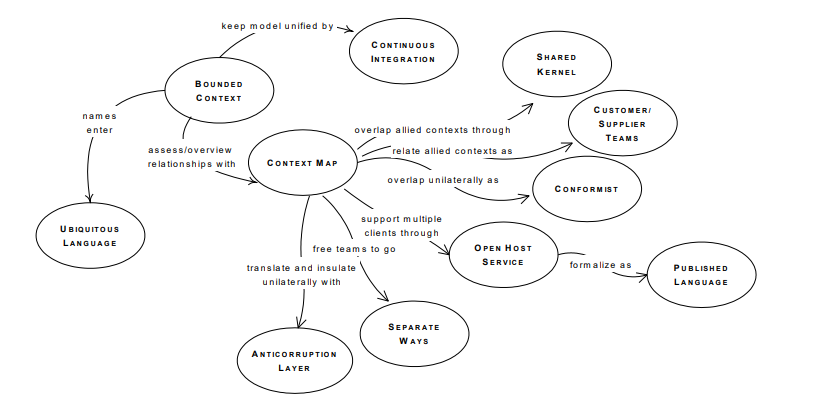
\includegraphics[width = 1\textwidth]{pictures/CacMoHinhChienLuoc/temp.png}

\caption{Sơ đồ về các thành phần trong mô hình chiến lược}

\end{figure}

%!<! - - $ Vẽ lại sau: - - >

%!<! - - $ Vẽ lại sau: - - >

%!<! - - $ Vẽ lại sau: - - >

%!<! - - $ Vẽ lại sau: - - >

%!<! - - $ Vẽ lại sau: - - >

%!<! - - $ Vẽ lại sau: - - >

%!<! - - $ Vẽ lại sau: - - >

%!<! - - $ Vẽ lại sau: - - >

%!<! - - $ Vẽ lại sau: - - >

%!<! - - $ Vẽ lại sau: - - >

%!<! - - $ Vẽ lại sau: - - >

%!<! - - Bối cảnh giới hạn (Bounded Context) - - >

%!<! - - [Giữ cho mô hình thống nhất] Tích hợp Liên tục (Continuous Integration) - - >

%!<! - - [Tính nhất quán trong trao đổi] Ngôn ngữ chung (Ubiquitous Language) - - >

%!<! - - [Tổng quan mối quan hệ] Bản đồ bối cảnh (Context Maps) - - >

%!<! - - Symmetric Relationship: Separate ways, Shared Kernel - - >

%!<! - - Asymmetric Relationship: Customer - Supplier, Conformist, Anti Corruption Layer - - >

%!<! - - - - >

%!<! - - One - to - Many Relationship: Open Host Service, Published Language - - >

%!<! - - dịch và cách ly đơn phương với - - >

%!<! - - [lớp] lớp (Context Maps) - - >

%

%!<! - - "Bản đồ bối cảnh dịch chuyển và cách ly một cách đơn phương để tạo thành cấu trúc lớp." - - >

%!<! - - Tách biệt - - >



% \subsubsection{Bối cảnh giới hạn (Bounded Context)}

% %!<! - - @ - - >

Một miền cần chia đủ nhỏ để phù hợp với một nhóm cụ thể. Để đạt được điều này, chúng ta cần xác định rõ ranh giới giữa các ngữ cảnh.

= > Bối cảnh giới hạn (Bounded Context) giúp định rõ các ranh giới, chia miền thành các phần độc lập để giải quyết sự phức tạp trong mô hình doanh nghiệp.

Bối cảnh giới hạn thể hiện phạm vi kinh doanh của dịch vụ.

![](pictures/BoiCanhGioiHan/___RanhGioi.png)

%!<! - - $VD: - - >
%!<! - - Một vài hướng xác định bối cảnh giới hạn: - - >

Việc xác định bối cảnh giới hạn được điều chỉnh bởi sự gắn kết giữa các miền phụ trong miền kinh doanh.
Dựa vào sơ đồ cấu trúc tổ chức của doanh nghiệp.
Dựa vào modules của các ứng dụng kiến trúc nguyên khối hiện tại (nếu việc phân chia tốt).
Dựa vào trách nhiệm và hoạt động của chuyên gia ngành.

%!<! - - Một số đặc điểm: - - >

Mỗi liên hệ giới hạn phải được thể hiện thông qua một mô hình miền riêng biệt không có sự chia sẻ về mô hình.

%!<! - - $VD: Hình mỗi domain có mô hình riêng... user(id, name) ở domain1, user(id, name, sdt) ở domain2 - - >

Những mô hình được tạo và quản lý độc lập bởi các nhóm.

%!<! - - $VD: - - >

Mô hình miền được xây dựng cho bối cảnh giới hạn chỉ có tác dụng trong phạm vi giới hạn của nó.

%!<! - - $VD: - - >
%!<! - - Hướng dẫn 5/10 - - >

% %!<! - - Bounded Context: https:// thiết kế hướng miền - practitioners.com/home/glossary/bounded - context - - >
% %!<! - - Bounded Context: https:// thiết kế hướng miền - practitioners.com/home/glossary/bounded - context - - >

Trang chủTrang chủBảng chú giảiBối cảnh giới hạn
Bối cảnh giới hạn
Trong thiết kế hướng miền (thiết kế hướng miền), bối cảnh giới hạn là ranh giới xác định phạm vi áp dụng một mô hình nhất định. Nó được sử dụng để tách biệt các mô hình khác nhau và tránh nhầm lẫn. Ý tưởng đằng sau bối cảnh giới hạn là tạo ra các mô hình khác nhau cho các khía cạnh khác nhau của miền và xác định rõ ràng ranh giới giữa chúng, sao cho các thuật ngữ giống nhau có thể được sử dụng với ý nghĩa khác nhau trong các ngữ cảnh khác nhau.

Ví dụ: một khách hàng có thể có nhiều ý nghĩa khác nhau tùy thuộc vào ngữ cảnh: trong ngữ cảnh thanh toán, đó là người nợ tiền; trong bối cảnh vận chuyển, đó là người nhận hàng. Bằng cách tạo một mô hình riêng cho từng ngữ cảnh, chúng ta có thể tránh nhầm lẫn và làm cho mã rõ ràng hơn.

Bối cảnh giới hạn được sử dụng để tạo bản đồ bối cảnh, hiển thị mối quan hệ giữa các mô hình khác nhau và cách chúng tương tác với nhau. Nó cũng giúp xác định các khu vực của miền cần có các mô hình khác nhau và xác định ranh giới giữa chúng.

Bối cảnh giới hạn cũng giúp cải thiện giao tiếp và cộng tác giữa các nhà phát triển, các bên liên quan và chuyên gia ngành bằng cách cung cấp ngôn ngữ chung và hiểu biết chung về miền. Nó cũng thúc đẩy tính mô đun, khả năng bảo trì và khả năng thích ứng của mã.

Khi tạo bối cảnh giới hạn, điều quan trọng là xác định bối cảnh trong đó mô hình được áp dụng, xác định ranh giới của bối cảnh, tạo mô hình phù hợp với mô hình miền tổng thể và truyền đạt bối cảnh tới các bối cảnh khác và miền tổng thể.

% %!<! - - Bounded Context: https:// thiết kế hướng miền - practitioners.com/home/glossary/bounded - context - - >
% %!<! - - Bounded Context: https:// thiết kế hướng miền - practitioners.com/home/glossary/bounded - context - - >
[[Context]] The setting in which a word or statement appears that determines its meaning. See [[Bounded Context]].

Mỗi bounded context nên tương ứng với một nhóm hoặc bộ phận cụ thể trong tổ chức. Sự tương ứng này có thể giúp giảm thiểu sự hiểu lầm và tăng khả năng tương tác giữa các nhóm ngũ.

Ví dụ: khách hàng có thể có nhiều ý nghĩa khác nhau tùy thuộc vào ngữ cảnh: trong ngữ cảnh thanh toán, đó là người nợ tiền; trong bối cảnh vận chuyển, đó là người nhận hàng. Bằng cách tạo một mô hình riêng cho từng ngữ cảnh, chúng ta có thể tránh nhầm lẫn và làm cho mã rõ ràng hơn.

% %!<! - - Bounded Context Relationships : https:// thiết kế hướng miền - practitioners.com/bounded - context - relationship - - >
% %!<! - - Bounded Context Relationships : https:// thiết kế hướng miền - practitioners.com/bounded - context - relationship - - >

Trang chủTrang chủBảng chú giảiBối cảnh giới hạn Mối quan hệ bối cảnh giới hạn
Mối quan hệ bối cảnh giới hạn
Trong Thiết kế hướng miền (thiết kế hướng miền), bối cảnh giới hạn là ranh giới trong đó một mô hình miền cụ thể tồn tại và hợp lệ. Các ngữ cảnh giới hạn giúp xác định phạm vi của mô hình miền và thiết lập sự hiểu biết rõ ràng về ngôn ngữ được sử dụng trong ngữ cảnh đó.

Các bối cảnh giới hạn phải độc lập trong bối cảnh riêng của chúng, nhưng chúng vẫn có thể cần tương tác với các bối cảnh giới hạn khác để hoàn thành trách nhiệm của chính chúng. Mặc dù chúng độc lập về mặt mô hình nhưng chúng có thể cần giao tiếp với các bối cảnh giới hạn khác để trao đổi thông tin hoặc cộng tác trong một số nhiệm vụ nhất định. Vì vậy các bối cảnh giới hạn có thể có mối quan hệ với nhau. Những mối quan hệ này rất quan trọng vì chúng giúp xác định sự tương tác giữa các phần khác nhau của hệ thống, cũng như thiết lập ranh giới và trách nhiệm giữa các nhóm khác nhau làm việc trên cùng một hệ thống. Có một số loại mối quan hệ bối cảnh giới hạn, bao gồm:

Quan hệ đối tác : Đây là mối quan hệ trong đó hai hoặc nhiều bối cảnh giới hạn cộng tác và chia sẻ thông tin. Mối quan hệ hợp tác có thể đạt được thông qua một sự kiện tích hợp hoặc bằng cách gọi một dịch vụ.
Hạt nhân được chia sẻ : Trong mối quan hệ này, hai bối cảnh giới hạn chia sẻ một lược đồ mô hình, mã hoặc CSDL chung. Các thành phần được chia sẻ phải ổn định, hoàn thiện và được cả hai nhóm đồng ý. Những thay đổi được thực hiện đối với các thành phần dùng chung cần phải được phối hợp cẩn thận để đảm bảo chúng không phá vỡ chức năng của bối cảnh khác.
Khách hàng - Nhà cung cấp : Đây là mối quan hệ trong đó một bối cảnh giới hạn cung cấp dịch vụ hoặc dữ liệu cho bối cảnh khác. Bối cảnh khách hàng dựa vào bối cảnh nhà cung cấp để có những khả năng hoặc dữ liệu nhất định. Những thay đổi trong bối cảnh nhà cung cấp có thể tác động đến bối cảnh khách hàng, vì vậy điều quan trọng là phải quản lý mối quan hệ này một cách cẩn thận.
Người theo chủ nghĩa tuân thủ : Mối quan hệ này tồn tại khi một bối cảnh giới hạn tuân theo cùng một ngôn ngữ và khái niệm phổ biến như một bối cảnh giới hạn khác. Điều này đảm bảo rằng giao tiếp giữa hai bối cảnh là rõ ràng và rõ ràng.
Lớp chống đổ vỡ : Đây là mối quan hệ trong đó ngữ cảnh được giới hạn sử dụng một lớp để dịch giữa ngôn ngữ của chính nó và ngôn ngữ của ngữ cảnh giới hạn khác. Điều này cho phép hai ngữ cảnh giao tiếp với nhau ngay cả khi chúng có từ vựng hoặc mô hình khác nhau.
Dịch vụ máy chủ mở : Mối quan hệ này xảy ra khi một bối cảnh giới hạn hiển thị một API công khai, mở mà các ngữ cảnh khác có thể sử dụng. Điều này cho phép các ngữ cảnh khác tận dụng chức năng của ngữ cảnh máy chủ theo cách được tiêu chuẩn hóa.
Ngôn ngữ được xuất bản : Trong mối quan hệ này, một ngữ cảnh giới hạn sẽ xuất bản từ vựng và mô hình của nó cho các ngữ cảnh khác sử dụng. Điều này hữu ích khi nhiều bối cảnh cần cộng tác nhưng không muốn tích hợp trực tiếp. Ngôn ngữ được xuất bản đảm bảo rằng ý nghĩa của các thuật ngữ nhất quán trong mọi ngữ cảnh.
Các cách riêng biệt : Mối quan hệ này đề cập đến tình huống trong đó hai hoặc nhiều bối cảnh giới hạn không còn có mối quan hệ với nhau và các nhóm chịu trách nhiệm về chúng chọn làm việc độc lập.

% %!<! - - Bounded Context Relationships : https:// thiết kế hướng miền - practitioners.com/bounded - context - relationship - - >
% %!<! - - Bounded Context Relationships : https:// thiết kế hướng miền - practitioners.com/bounded - context - relationship - - >

% \subsubsection{CI/CD}

% %!<! - - @Tích hợp Liên tục (Continuous Integration) - - >

Tích hợp Liên tục (Continuous Integration): là việc các thành viên trong nhóm phát triển tích hợp mã nguồn vào một hệ thống chung thường xuyên. Khi có mã nguồn mới việc tích hợp liên tục sẽ tự động kiểm thử và xây dựng giảm xung đột giữa các phiên bản mã nguồn khác nhau, giúp phát hiện và sửa lỗi sớm hơn.
% CD là gì
% CD là gì
% CD là gì
% CD là gì
% CD là gì
% CD là gì
% CD là gì
% CD là gì
% CD là gì
CI/CD là viết tắt của hai khái niệm quan trọng trong quá trình phát triển phần mềm: Continuous Integration (CI) và Continuous Delivery (CD). Đây là một phương pháp giúp tự động hóa quy trình phát triển, kiểm thử, và triển khai ứng dụng, giúp tăng cường chất lượng phần mềm và giảm thời gian cũng như rủi ro trong quá trình phát triển.

1. **Continuous Integration (CI - Tích hợp liên tục):**
- **Mục tiêu:** Đảm bảo rằng mã nguồn mới được tích hợp vào mã nguồn chính (main codebase) một cách tự động và thường xuyên, giảm thời gian giữa việc viết mã và phát hành.
- **Quy trình:** Mỗi khi một nhà phát triển hoàn thành một tính năng hoặc sửa lỗi, họ tích hợp mã của mình vào mã nguồn chính. Hệ thống CI sẽ tự động kiểm tra mã này bằng cách chạy các bài kiểm thử tự động để đảm bảo rằng nó không làm hỏng hệ thống.

2. **Continuous Delivery (CD - Phân phối liên tục):**
- **Mục tiêu:** Tự động hóa việc triển khai ứng dụng để có thể phân phối bản vá, tính năng hoặc cập nhật một cách nhanh chóng và đáng tin cậy.
- **Quy trình:** Nếu quá trình CI thành công, mã nguồn sẽ được triển khai tự động lên môi trường thử nghiệm (staging environment). Nếu mọi thứ ổn, nó có thể được triển khai tự động lên môi trường sản phẩm (production environment).

3. **Continuous Deployment (CD - Triển khai liên tục):**
- **Khác biệt với Continuous Delivery:** Trong Continuous Deployment, nếu mọi thứ qua bài kiểm thử được tự động và thành công, mã nguồn sẽ tự động triển khai lên môi trường sản phẩm mà không cần sự can thiệp thủ công.
- **Mục tiêu:** Tối ưu hóa quá trình triển khai, giảm thiểu sự chờ đợi và đảm bảo tính ổn định của hệ thống.

4. **Các công cụ thường được sử dụng:**
- **Jenkins, Travis CI, CircleCI:** Đối với CI.
- **Docker, Kubernetes:** Đối với CD, đặc biệt là việc triển khai và quản lý containerized applications.
- **Ansible, Puppet, Chef:** Công cụ tự động hóa cấu hình và triển khai.

Tổng cộng, CI/CD giúp tăng cường khả năng linh hoạt, đảm bảo chất lượng mã nguồn, giảm rủi ro, và giảm thời gian giữa việc phát triển và triển khai sản phẩm.

% CD là gì
% CD là gì
% CD là gì
% CD là gì
% CD là gì
% CD là gì
% CD là gì
% CD là gì
% CD là gì
% CD là gì

Khi một bối cảnh giới hạn đã được xác định, chúng ta cần đảm bảo rằng nó luôn ở trạng thái mới và hoạt động tốt như kỳ vọng. Đáp ứng nhu cầu doanh nghiệp phát triển thay đổi liên tục và nhanh chóng.
Khi cùng vận hành và phát triển xung đột có thể xảy ra ở cùng hoặc khác bối cảnh giới hạn.
= > Vì vậy, cần sử dụng việc tích hợp liên tục tạo ra một quy trình tự động và liên tục từ việc tích hợp mã nguồn, kiểm thử tự động giúp tăng cường chất lượng phần mềm, giảm thời gian và rủi ro trong quá trình phát triển phần mềm.

%!<! - - $VD: jenkins - - >
%!<! - - unit test - - >
%!<! - - test tích hợp - - >

% vở
% thời gian khác nhau

% http://localhost nên không có CD

% \subsubsection{Ngôn ngữ chung (Ubiquitous Language)}

% %!<! - - @ - - >

Trong quá trình xây dựng mô hình miền, cần có đối thoại trao đổi giữa những người thiết kế phần mềm và chuyên gia ngành để hiểu đúng về miền. Tuy nhiên, nhóm kinh doanh sử dụng ngôn ngữ kinh doanh và nhóm công nghệ có xu hướng sử dụng các thuật ngữ kỹ thuật trong giao tiếp của họ. Người phát triển phần mềm tập trung vào lớp, phương thức, thuật toán, trong khi chuyên gia ngành thường sử dụng ngôn ngữ chuyên ngành của họ. Sự khác biệt về ngôn ngữ giữa các thành viên có thể dẫn đến những thách thức về giao tiếp.

Trong các lĩnh vực kinh doanh khác nhau, một thuật ngữ có thể được sử dụng trong nhiều miền, cùng với ý nghĩa khác nhau gây ra sự nhầm lẫn và hiểu sai cho các người phát triển phần mềm cũng như các chuyên gia ngành.

%!<! - - = > Thiết kế hướng miền đề xuất sử dụng ngôn ngữ chung để giải quyết những thách thức ngôn ngữ. - - >

Ngôn ngữ chung (Ubiquitous Language) là một trong những mô hình chiến lược của thiết kế hướng miền, thiết lập một ngôn ngữ chung trong từng bối cảnh kinh doanh.
Ngôn ngữ chung được xác định bởi từ vựng và có định nghĩa rõ ràng về ngữ cảnh từ vựng áp dụng.

%!<! - - Một số đặc điểm: - - >

Ngôn ngữ chung được sử dụng bởi cả chuyên gia ngành và chuyên gia công nghệ.
Có nhiều ngôn ngữ chung trong một tổ chức được mỗi nhóm tạo và quản lý một cách độc lập.
Việc tạo ra ngôn ngữ chung là một quá trình liên tục. Ngôn ngữ chung phát triển theo thời gian thông qua sự cộng tác giữa doanh nghiệp và các chuyên gia công nghệ.

Các thành viên phải sử dụng ngôn ngữ chung cho công việc và trong toàn bộ hệ thống như:

Sử dụng trong cuộc thảo luận trao đổi giữa các chuyên gia ngành và các chuyên gia công nghệ
Sử dụng trong các tài liệu phát triển của nhóm
Sử dụng trong sản phẩm và kiểm thử phần mềm

![](pictures/NgonNguChung/___NgonNguPhoBien.png)

%!<! - - $VD: Ngôn ngữ chung được sử dụng, áp dụng trong toàn bộ hệ thống. - - >
%!<! - - Hướng dẫn 5/7 - - >

%!<! - - [[Ubiquitous Language]] A language structured around the domain model and used by all team members to connect all the activities of the team with the software. - - >
% %!<! - - Ubiquitous Language : https:// thiết kế hướng miền - practitioners.com/home/glossary/ubiquitous - language - - >
% %!<! - - Ubiquitous Language : https:// thiết kế hướng miền - practitioners.com/home/glossary/ubiquitous - language - - >
% %!<! - - Ubiquitous Language : https:// thiết kế hướng miền - practitioners.com/home/glossary/ubiquitous - language - - >
% %!<! - - Ubiquitous Language : https:// thiết kế hướng miền - practitioners.com/home/glossary/ubiquitous - language - - >
% %!<! - - Ubiquitous Language : https:// thiết kế hướng miền - practitioners.com/home/glossary/ubiquitous - language - - >
% %!<! - - Ubiquitous Language : https:// thiết kế hướng miền - practitioners.com/home/glossary/ubiquitous - language - - >
% %!<! - - Ubiquitous Language : https:// thiết kế hướng miền - practitioners.com/home/glossary/ubiquitous - language - - >

Trang chủTrang chủBảng chú giải ngôn ngữ chung
ngôn ngữ chung
Trong thiết kế hướng miền (thiết kế hướng miền), ngôn ngữ chung là ngôn ngữ dùng chung được sử dụng để mô tả miền và mô hình miền. Đó là ngôn ngữ chung được các nhà phát triển, các bên liên quan và chuyên gia ngành sử dụng để giao tiếp và hiểu miền kinh doanh.

Ý tưởng đằng sau ngôn ngữ chung là tạo ra sự hiểu biết chung về miền bằng cách sử dụng một ngôn ngữ chung để mô tả các khái niệm và mối quan hệ trong miền. Ngôn ngữ chung này nên được sử dụng nhất quán trong suốt quá trình phát triển phần mềm, từ giai đoạn phân tích và thiết kế đến giai đoạn triển khai và bảo trì.

ngôn ngữ chung phải dựa trên ngôn ngữ đã được sử dụng trong miền và nên được sử dụng để đặt tên cho các lớp, giao diện, phương thức và biến trong mã. Điều này giúp đảm bảo rằng mã có tính biểu cảm, dễ hiểu và phù hợp với nhu cầu kinh doanh.

Mục tiêu của ngôn ngữ chung là đảm bảo rằng phần mềm phù hợp với nhu cầu kinh doanh và miền kinh doanh được thể hiện chính xác trong phần mềm. Nó cũng giúp cải thiện khả năng giao tiếp và cộng tác giữa các nhóm khác nhau và đảm bảo rằng phần mềm có thể bảo trì và thích ứng với sự thay đổi.

Điều quan trọng cần lưu ý là ngôn ngữ chung không chỉ giới hạn ở cách đặt tên mã mà còn là một cách để đảm bảo rằng các khái niệm và mối quan hệ kinh doanh được thể hiện chính xác trong phần mềm và phần mềm phù hợp với nhu cầu kinh doanh.

Dưới đây là một số ví dụ về cách áp dụng ngôn ngữ chung trong thiết kế hướng miền:

Quy ước đặt tên : Tên của các lớp, giao diện, phương thức và biến trong mã phải dựa trên ngôn ngữ đã được sử dụng trong miền. Ví dụ: trong miền thương mại điện tử, khái niệm “đặt hàng” phải được gọi một cách nhất quán là “đặt hàng” trong toàn bộ mã, thay vì sử dụng các tên khác nhau như “mua hàng” hoặc “giao dịch”.
Mô hình hóa quy trình nghiệp vụ : Các quy trình nghiệp vụ trong miền phải được mô hình hóa bằng cách sử dụng cùng các thuật ngữ và khái niệm đã được sử dụng trong miền. Ví dụ: trong lĩnh vực chăm sóc sức khỏe, quy trình “tiếp nhận bệnh nhân” phải được đề cập đến việc sử dụng các thuật ngữ và khái niệm tương tự được các chuyên gia chăm sóc sức khỏe sử dụng, chẳng hạn như “quy trình tiếp nhận” hoặc “quy trình đăng ký bệnh nhân”
Mô hình hóa các thực thể kinh doanh : Các thực thể kinh doanh trong miền phải được mô hình hóa bằng cách sử dụng cùng các thuật ngữ và khái niệm đã được sử dụng trong miền. Ví dụ: trong lĩnh vực tài chính, khái niệm “tài khoản” phải được gọi một cách nhất quán là “tài khoản” trong toàn bộ mã, thay vì sử dụng các tên khác nhau như “sổ cái” hoặc “hồ sơ tài chính”
Giao tiếp : ngôn ngữ chung nên được sử dụng trong mọi giao tiếp, bao gồm các cuộc họp, tài liệu và nhận xét mã, để đảm bảo rằng mọi người đều sử dụng các thuật ngữ và khái niệm giống nhau.

% %!<! - - Ubiquitous Language : https:// thiết kế hướng miền - practitioners.com/home/glossary/ubiquitous - language - - >
% %!<! - - Ubiquitous Language : https:// thiết kế hướng miền - practitioners.com/home/glossary/ubiquitous - language - - >
% %!<! - - Ubiquitous Language : https:// thiết kế hướng miền - practitioners.com/home/glossary/ubiquitous - language - - >
% %!<! - - Ubiquitous Language : https:// thiết kế hướng miền - practitioners.com/home/glossary/ubiquitous - language - - >

%!<! - - Bằng cách sử dụng ngôn ngữ chung như trên, chúng ta có thể tạo ra một mô hình thiết kế hướng miền rõ ràng và dễ hiểu, giúp các nhóm phát triển, quản lý dự án và người dùng hiểu rõ về các yêu cầu và chức năng của hệ thống. - - >

% \subsubsection{Bản đồ bối cảnh (Context Maps)}

% 
Trong kiến trúc kiến trúc vi dịch vụ, các dịch vụ phải tương tác quan hệ với nhau, dẫn đến sự xuất hiện của mối quan hệ phụ thuộc. Những mối quan hệ này cần được quản lý chặt chẽ. Nếu không thì các dịch vụ sẽ mất khả năng hoạt động độc lập, tính nhất quán và tính linh hoạt.

= > Do đó, các nhóm phải nỗ lực để ghi lại mối quan hệ giữa các quan hệ thông qua việc sử dụng bản đồ bối cảnh.

Bản đồ bối cảnh (Context Maps) là sự thể hiện trực quan của hệ thống, thể hiện các thành phần, liên kết và mối quan hệ.

![](pictures/BanDoBoiCanh/image.png)

%!<! - - $VD: Bản đồ bối cảnh - - >

%!<! - - Lợi ích của Bản đồ bối cảnh: - - >

Giúp thành viên trong nhóm hiểu rõ hơn về bức tranh toàn cảnh.

Giúp nhận biết sự phụ thuộc lẫn nhau giữa các liên hệ giới hạn.

Giúp các nhóm đánh giá mức độ hợp tác với các nhóm khác.

Giúp sàng lọc các liên hệ giới hạn và các mô hình.

Xác định mối quan hệ giữa các liên hệ giới hạn của mình.

%!<! - - @ Visual Representation
[[Context Map]] A representation of the [[Bounded Context]]s involved in a project and the actual relationships between them and their models.
[[Bản đồ bối cảnh]] Sự thể hiện của [[Bounded Context]] tham gia vào một dự án và các mối quan hệ thực tế giữa chúng và các mô hình của chúng.

Hữu ích cho việc hiểu kiến trúc tổng thể

% %!<! - - Context Mapping : https:// thiết kế hướng miền - practitioners.com/context - map - - >

% %!<! - - Context Mapping : https:// thiết kế hướng miền - practitioners.com/context - map - - >

% %!<! - - Context Mapping : https:// thiết kế hướng miền - practitioners.com/context - map - - >

% %!<! - - Context Mapping : https:// thiết kế hướng miền - practitioners.com/context - map - - >

% %!<! - - Context Mapping : https:// thiết kế hướng miền - practitioners.com/context - map - - >

% %!<! - - Context Mapping : https:// thiết kế hướng miền - practitioners.com/context - map - - >

% %!<! - - Context Mapping : https:// thiết kế hướng miền - practitioners.com/context - map - - >

Trang chủTrang chủBảng chú giảiBản đồ bối cảnh

Bản đồ bối cảnh

Trong Thiết kế hướng miền, Bản đồ bối cảnh là một công cụ trực quan được sử dụng để hiển thị mối quan hệ giữa các bối cảnh giới hạn khác nhau trong một miền. Về cơ bản, nó là một bản đồ hiển thị cách các bối cảnh khác nhau trong một miền tương tác với nhau, bao gồm ranh giới, sự phụ thuộc và kiểu giao tiếp của chúng.

Bối cảnh giới hạn rất quan trọng trong thiết kế hướng miền vì chúng giúp xác định và quản lý độ phức tạp của các miền lớn bằng cách chia chúng thành các phần nhỏ hơn, dễ quản lý hơn. Bằng cách hiểu mối quan hệ giữa các bối cảnh khác nhau, các nhóm phát triển có thể cộng tác hiệu quả hơn và đảm bảo rằng mỗi bối cảnh được thiết kế theo cách phù hợp với mục tiêu chung của miền. Bản đồ bối cảnh cũng giúp làm nổi bật các khu vực có xung đột hoặc chồng chéo tiềm ẩn giữa các bối cảnh, có thể được giải quyết sớm để tránh các vấn đề về sau.

Bản đồ ngữ cảnh thường bao gồm các thành phần sau:

Ngữ cảnh : Một miền hoặc miền phụ cụ thể có ngữ cảnh giới hạn với các ranh giới rõ ràng và ngôn ngữ chung được xác định rõ ràng.

Bối cảnh giới hạn : Một ranh giới xác định một miền hoặc miền phụ cụ thể trong đó các thuật ngữ và khái niệm có ý nghĩa cụ thể.

Mối quan hệ : Các mối quan hệ giữa các bối cảnh giới hạn. Ở mức độ rộng hơn, các mối quan hệ có hai loại: đối xứng hoặc bất đối xứng. Trong một mối quan hệ đối xứng, cả hai bên đều có tiếng nói ít nhiều bình đẳng trong việc mối quan hệ phát triển như thế nào. Trong mối quan hệ bất đối xứng, một bên đóng vai trò là trung tâm quyền lực rõ ràng

Nhóm : Các nhóm chịu trách nhiệm phát triển và duy trì bối cảnh hoặc miền phụ giới hạn.

Mục tiêu chiến lược : Các mục tiêu chiến lược mà mỗi bối cảnh giới hạn hướng tới đạt được.

Bản đồ bối cảnh cung cấp chế độ xem cấp cao về miền và cách các bối cảnh giới hạn khác nhau có liên quan với nhau, giúp các bên liên quan xác định kiến trúc, sự phụ thuộc và rủi ro của hệ thống.

Có một số loại mối quan hệ có thể được mô tả trên bản đồ ngữ cảnh, bao gồm:

Quan hệ đối tác : Mối quan hệ giữa hai bối cảnh giới hạn trong đó họ cộng tác như những đối tác bình đẳng để đạt được mục tiêu chung.

Hạt nhân được chia sẻ : Mối quan hệ trong đó hai bối cảnh giới hạn chia sẻ một phần của mô hình miền hoặc nguồn dữ liệu.

Khách hàng - Nhà cung cấp : Mối quan hệ giữa hai bối cảnh giới hạn trong đó một bối cảnh cung cấp chức năng hoặc dữ liệu cho bối cảnh khác, ngữ cảnh này sử dụng nó.

Người theo chủ nghĩa tuân thủ : Một mối quan hệ trong đó một bối cảnh được liên kết với một bối cảnh khác và tuân thủ các quy tắc, tiêu chuẩn hoặc chính sách của bối cảnh đó.

Lớp chống đổ vỡ : Mối quan hệ trong đó lớp dịch được sử dụng để tách biệt ngữ cảnh này với ngữ cảnh khác bằng mô hình hoặc công nghệ không tương thích.

Dịch vụ máy chủ mở : Một mối quan hệ trong đó bối cảnh giới hạn cung cấp API công khai có thể được sử dụng bởi các máy khách bên ngoài hoặc các bối cảnh giới hạn khác.

Ngôn ngữ được xuất bản : Một mối quan hệ trong đó hai bối cảnh giới hạn đồng ý về một ngôn ngữ hoặc từ vựng chung để giao tiếp với nhau.

Các cách riêng biệt : Một mối quan hệ trong đó hai bối cảnh giới hạn hoàn toàn độc lập và không có tương tác với nhau.

Ví dụ

Đây là bản đồ bối cảnh đơn giản hóa cho một ngân hàng XYZ hư cấu. Hình ảnh này mô tả các bối cảnh giới hạn khác nhau, mối quan hệ của chúng. Trong trường hợp mối quan hệ không đối xứng, nó cũng chỉ ra bên nào là thượng nguồn và hạ lưu. Nhìn vào hình ảnh này sẽ giúp người xem có cái nhìn rõ ràng về bức tranh tổng thể về bất động sản phần mềm tại Ngân hàng XYZ.

So sánh với mô hình C4

Mô hình C4 cung cấp một cách khác để mô tả kiến trúc giải pháp của chúng ta. Cụ thể, sơ đồ ngữ cảnh hệ thống về bản chất rất giống với sơ đồ ngữ cảnh ở chỗ chúng đều được sử dụng để trực quan hóa kiến trúc của một hệ thống phần mềm. Tuy nhiên, có một số khác biệt chính giữa hai cách tiếp cận.

Bản đồ bối cảnh thiết kế hướng miền là một sơ đồ cấp cao hiển thị các bối cảnh giới hạn khác nhau trong một hệ thống. Mỗi ngữ cảnh giới hạn là một miền độc lập có ngôn ngữ, mô hình và dịch vụ riêng. Bản đồ bối cảnh thiết kế hướng miền là một công cụ hữu ích để hiểu kiến trúc tổng thể của một hệ thống và cách các bối cảnh giới hạn khác nhau tương tác với nhau.

Sơ đồ ngữ cảnh hệ thống của mô hình C4 là sơ đồ chi tiết hơn hiển thị các vùng chứa và thành phần khác nhau trong hệ thống. Mỗi container là một nhóm các thành phần có chung cơ sở hạ tầng. Sơ đồ ngữ cảnh hệ thống của mô hình C4 là một công cụ hữu ích để hiểu kiến trúc bên trong của hệ thống cũng như cách các vùng chứa và thành phần khác nhau tương tác với nhau.

Dưới đây là bảng tóm tắt những khác biệt chính giữa hai phương pháp:

Bản đồ bối cảnh thiết kế hướng miền 	Sơ đồ ngữ cảnh hệ thống của mô hình C4

Hiển thị các bối cảnh giới hạn khác nhau	Hiển thị các vùng chứa và thành phần khác nhau

Sơ đồ cấp cao	Sơ đồ chi tiết hơn

Hữu ích cho việc hiểu kiến trúc tổng thể	Hữu ích cho việc hiểu kiến trúc nội bộ 

% ĐẾN ĐÂY
% ĐẾN ĐÂY
% ĐẾN ĐÂY
% ĐẾN ĐÂY
% ĐẾN ĐÂY
% ĐẾN ĐÂY
% ĐẾN ĐÂY
% ĐẾN ĐÂY
% ĐẾN ĐÂY
% ĐẾN ĐÂY

% \subsubsection{Chi tiết về các mối quan hệ bối cảnh giới hạn}

% Có 3 loại mối quan hệ bối cảnh giới hạn là:
- xxxxxxxxxxxxxxx
- xxxxxxxxxxxxxxx
- xxxxxxxxxxxxxxx

\paragraph{Mối quan hệ đối xứng (Symmetric Relationship)}

% \subparagraph{Mô hình riêng biệt (Separate Ways)}

% % khi quan hệ riêng biệt, không có sự phụ thuộc lẫn nhau.

Các liên hệ trong bối cảnh giới hạn thực sự độc lập.

Các liên hệ không có mối quan hệ nào với các liên hệ khác.

Các liên hệ có mô hình độc lập và thực thi riêng biệt.

Các nhóm phát triển không phải cộng tác hay phối hợp cho bất kỳ nhiệm vụ nào.

% %! $VD: trong trường hợp ngân hàng, thẻ tín dụng và khoản vay mua nhà không có mối quan hệ nào. - - >

% %! Separate Ways : https:// thiết kế hướng miền - practitioners.com/separate - ways - - >

% %! Separate Ways : https:// thiết kế hướng miền - practitioners.com/separate - ways - - >

Trang chủTrang chủBảng chú giảiBối cảnh giới hạn Mối quan hệ bối cảnh giới hạn Đường riêng

Đường riêng

Loại mối quan hệ này đề cập đến tình huống trong đó hai hoặc nhiều bối cảnh giới hạn quá khác nhau về mục đích, ngôn ngữ hoặc lĩnh vực đến mức chúng không thể hoặc không nên được tích hợp hoặc liên kết với nhau. Nói cách khác, họ cần đi theo con đường riêng và độc lập với nhau. Quyết định này thường được đưa ra khi thấy rõ rằng lợi ích của việc cố gắng điều chỉnh hoặc tích hợp các bối cảnh giới hạn sẽ lớn hơn chi phí hoặc rủi ro liên quan. Trong những trường hợp như vậy, các nhóm chịu trách nhiệm về từng bối cảnh giới hạn nên tập trung vào miền, ngôn ngữ và mô hình của riêng họ, đồng thời tránh sự phụ thuộc hoặc giả định về các bối cảnh giới hạn khác.

Hàm ý

Những ưu và nhược điểm của việc đi theo những con đường riêng biệt bao gồm:

Ưu điểm

Cải thiện khả năng bảo trì: Các thành phần nhỏ hơn, tập trung hơn sẽ dễ bảo trì, sửa đổi và mở rộng quy mô hơn.

Ranh giới rõ ràng: Mỗi bối cảnh được giới hạn đều có ranh giới được xác định rõ ràng, giúp ngăn ngừa sự nhầm lẫn và xung đột giữa các yêu cầu.

Triển khai độc lập: Các bối cảnh giới hạn có thể được triển khai và thử nghiệm độc lập, điều này có thể tăng tốc chu kỳ phát triển và triển khai.

Khuyến khích thiết kế theo miền: Quá trình tạo bối cảnh giới hạn có thể giúp các nhóm tập trung vào các khái niệm miền cốt lõi và đảm bảo rằng mỗi thành phần đều phù hợp với mục tiêu kinh doanh tổng thể.

Nhược điểm

Độ phức tạp ngày càng tăng: Việc chia hệ thống thành nhiều bối cảnh có giới hạn có thể tạo thêm độ phức tạp vì các nhà phát triển phải quản lý sự tương tác và giao tiếp giữa các thành phần.

Khả năng xảy ra những nỗ lực trùng lặp: Các nhóm khác nhau có thể cần phát triển chức năng tương tự trong bối cảnh giới hạn tương ứng của họ, điều này có thể dẫn đến những nỗ lực trùng lặp và tăng chi phí bảo trì.

Thách thức về tích hợp: Khi các bối cảnh giới hạn phát triển và thay đổi theo thời gian, việc tích hợp chúng vào hệ thống lớn hơn có thể gặp khó khăn, đặc biệt nếu các tương tác giữa các thành phần phức tạp.

Tăng cường phối hợp: Sự phối hợp và giao tiếp hiệu quả giữa các nhóm là rất quan trọng để đảm bảo rằng mỗi bối cảnh giới hạn đều phù hợp với mục tiêu kinh doanh tổng thể và hoạt động liền mạch với các thành phần khác.

Đi theo những cách riêng biệt có thể là một cách tiếp cận hiệu quả để quản lý các hệ thống phức tạp, nhưng nó đòi hỏi phải lập kế hoạch và phối hợp cẩn thận để đảm bảo rằng mỗi bối cảnh giới hạn hoạt động tốt với những bối cảnh khác và phù hợp với các mục tiêu kinh doanh tổng thể.

% %! Separate Ways : https:// thiết kế hướng miền - practitioners.com/separate - ways - - >

% %! Separate Ways : https:// thiết kế hướng miền - practitioners.com/separate - ways - - >

% \subparagraph{Mô hình hợp tác (Partnership)}

% % Khi những liên hệ giới hạn có sự phụ thuộc lẫn nhau.
% Đôi khi chúng ta tìm thấy những liên hệ giới hạn có sự phụ thuộc lẫn nhau.
**Mô hình hợp tác (Partnership Pattern)**
Sự phụ thuộc lẫn nhau này dẫn đến mức độ kết hợp cao.
Từ góc độ hiện thực hóa, mô hình hợp tác chuyển thành các dịch vụ có sự phụ thuộc lẫn nhau.
= > Vì vậy, các nhóm không thể hoạt động độc lập.
Mỗi nhóm tham gia vào mối quan hệ này sẽ cần phải tìm hiểu các mô hình kinh doanh và ngôn ngữ chung cho các mối liên hệ gắn kết do nhóm kia quản lý.
= > Sự phụ thuộc cao dẫn tới mất đi tính độc lập của kiến trúc vi dịch vụ.

Một cách để giải quyết vấn đề này là phân định ranh giới cho các mô hình dùng chung.
Có thể tạo ranh giới xung quanh các mô hình được chia sẻ giữa hai điểm tiếp xúc được liên kết.
Quản lý các mô hình chia sẻ này một cách độc lập với phần còn lại của bối cảnh liên kết.
Nếu cần thay đổi và thay đổi không phải là một phần của mô hình được chia sẻ thì nhóm được đưa ra quyết định độc lập.
Nhưng nếu có nhu cầu thay đổi mẫu dùng chung thì 2 nhóm sẽ phối hợp.

% %! Partnership : https:// thiết kế hướng miền - practitioners.com/partnership - - >
% %! Partnership : https:// thiết kế hướng miền - practitioners.com/partnership - - >
% %! Partnership : https:// thiết kế hướng miền - practitioners.com/partnership - - >

Trang chủTrang chủBảng chú giảiBối cảnh giới hạn Mối quan hệ bối cảnh giới hạn quan hệ đối tác
quan hệ đối tác
Trong Thiết kế hướng miền (thiết kế hướng miền), mối quan hệ hợp tác là một loại mối quan hệ giữa các bối cảnh giới hạn . Trong mối quan hệ này, hai hoặc nhiều bối cảnh giới hạn cộng tác theo cách mà chúng có sự hiểu biết chung về mô hình của nhau và cách chúng tương tác với nhau. Mục tiêu của sự hợp tác này là cung cấp giải pháp đầy đủ và toàn diện cho vấn đề miền mà hệ thống đang giải quyết.

Trong mối quan hệ hợp tác, các bối cảnh giới hạn không hoàn toàn độc lập với nhau nhưng vẫn duy trì một mức độ tự chủ và độc lập nhất định. Sự hợp tác giữa họ dựa trên mô hình miền chung, được tất cả những người tham gia hợp tác đồng ý. Mô hình này hoạt động như một ngôn ngữ chung cho phép các nhóm khác nhau giao tiếp hiệu quả và xây dựng các giải pháp phối hợp hiệu quả với nhau.

Mối quan hệ hợp tác rất hữu ích khi các bối cảnh giới hạn cần chia sẻ dữ liệu hoặc cộng tác để cung cấp giải pháp hoàn chỉnh cho vấn đề miền. Mối quan hệ này thường được thiết lập giữa các bối cảnh có liên quan chặt chẽ và có tác động đáng kể đến hành vi của nhau.

Hàm ý
Mối quan hệ hợp tác giữa các bối cảnh giới hạn có thể có cả ưu điểm và nhược điểm:

Ưu điểm
Mối quan hệ hợp tác có thể tạo điều kiện thuận lợi cho việc giao tiếp và cộng tác giữa các nhóm làm việc trên các bối cảnh giới hạn khác nhau.
Chúng có thể giúp điều chỉnh ngôn ngữ chung và đảm bảo rằng các mô hình khác nhau đều nhất quán và bổ sung cho nhau.
Chúng có thể cho phép tạo ra các giải pháp toàn diện, gắn kết hơn, trải rộng trên nhiều bối cảnh giới hạn .
Chúng có thể tạo cơ hội cho việc tái sử dụng các dịch vụ hoặc thành phần trong nhiều ngữ cảnh.
Nhược điểm
Mối quan hệ hợp tác có thể tạo ra sự phụ thuộc giữa các nhóm và bối cảnh giới hạn, điều này có thể gây khó khăn hơn cho việc phát triển toàn bộ hệ thống.
Họ có thể giới thiệu thêm chi phí liên lạc và phối hợp.
Chúng có thể khiến việc duy trì quyền tự chủ và độc lập của các bối cảnh giới hạn trở nên khó khăn hơn.
Chúng có thể làm tăng độ phức tạp của toàn bộ hệ thống và khiến việc giải thích trở nên khó khăn hơn.
Ví dụ
Giả sử chúng ta có bối cảnh giới hạn cho nền tảng thương mại điện tử, bao gồm tổng hợp Giỏ hàng xử lý tất cả logic liên quan đến việc thêm mặt hàng vào giỏ hàng, cập nhật số lượng và xử lý đơn đặt hàng. Một bối cảnh giới hạn khác trong hệ thống là dịch vụ Xử lý thanh toán chịu trách nhiệm xử lý các khoản thanh toán.

Trong trường hợp này, chúng ta có thể thiết lập mối quan hệ hợp tác giữa bối cảnh Giỏ hàng và Xử lý thanh toán. Điều này có nghĩa là khi một đơn đặt hàng được gửi trong ngữ cảnh Giỏ hàng, ngữ cảnh Xử lý Thanh toán sẽ được thông báo và có thể bắt đầu xử lý thanh toán. Nếu thanh toán thành công, bối cảnh Giỏ hàng sẽ được thông báo để nó có thể hoàn tất đơn hàng, nhưng nếu thanh toán không thành công, bối cảnh Giỏ hàng có thể thực hiện các hành động đền bù để hủy đơn hàng.

Mối quan hệ hợp tác này cho phép hai bối cảnh giới hạn làm việc cùng nhau để hoàn thành một mục tiêu chung, trong khi vẫn duy trì cấu trúc dữ liệu và logic độc lập của riêng chúng. Nhược điểm của phương pháp này là nó có thể làm tăng thêm độ phức tạp và sự phụ thuộc giữa các ngữ cảnh, vì vậy nó nên được sử dụng một cách thận trọng và chỉ khi cần thiết.

Khi nào nó hoạt động?
Để mối quan hệ hợp tác giữa các bối cảnh giới hạn hoạt động hiệu quả, cần phải đáp ứng các điều kiện sau:

Ngôn ngữ miền dùng chung: Cả hai ngữ cảnh được giới hạn phải thống nhất về ngôn ngữ và thuật ngữ được sử dụng để mô tả các khái niệm và hoạt động của miền.
Hợp tác mạnh mẽ: Sự hợp tác hiệu quả giữa các nhóm chịu trách nhiệm về từng bối cảnh giới hạn là điều cần thiết. Cần có sự giao tiếp rõ ràng và tương tác thường xuyên để đảm bảo sự thống nhất giữa các mục tiêu và hoạt động.
Ranh giới rõ ràng: Ranh giới của từng bối cảnh được giới hạn cần được xác định rõ ràng để tránh chồng chéo, nhầm lẫn.
Bản đồ bối cảnh rõ ràng: Mối quan hệ giữa các bối cảnh giới hạn phải được ghi lại rõ ràng, bao gồm các tương tác giữa các nhóm chịu trách nhiệm về từng bối cảnh giới hạn và các quy tắc quản lý các tương tác đó.
Tính nhất quán và ổn định: Giao diện giữa các bối cảnh giới hạn phải ổn định và nhất quán theo thời gian để tránh gián đoạn mối quan hệ.
Lợi ích chung: Cả hai bối cảnh đều phải thu được lợi ích chung từ quan hệ đối tác. Điều này có thể bao gồm việc chia sẻ dữ liệu hoặc chức năng hoặc phân phối giá trị doanh nghiệp hiệu quả hơn.
Khi nào nó không hoạt động?
Mối quan hệ hợp tác có thể không hoạt động trong các trường hợp sau:

Thiếu tin tưởng: Trong mối quan hệ hợp tác, mỗi bối cảnh giới hạn nên tin tưởng người kia sẽ hoàn thành trách nhiệm của mình. Nếu thiếu sự tin tưởng có thể dẫn đến xung đột, hiểu lầm.
Mục tiêu không phù hợp: Nếu mục tiêu của các bối cảnh giới hạn không được căn chỉnh, có thể dẫn đến xung đột và bất đồng. Ví dụ: nếu một bối cảnh giới hạn tập trung vào việc tối ưu hóa tốc độ, trong khi ngữ cảnh còn lại tập trung vào tính nhất quán của dữ liệu thì có thể xảy ra xung đột.
Vấn đề giao tiếp: Mối quan hệ hợp tác đòi hỏi sự giao tiếp và hợp tác hiệu quả giữa các nhóm. Nếu có vấn đề về giao tiếp hoặc sự khác biệt về văn hóa giữa các nhóm, điều đó có thể dẫn đến hiểu lầm và xung đột.
Đóng góp không đồng đều: Trong mối quan hệ hợp tác, cả hai bối cảnh đều phải đóng góp như nhau cho mục tiêu chung. Nếu một bối cảnh giới hạn đang thực hiện tất cả những công việc nặng nhọc trong khi bối cảnh kia không đóng góp đủ, điều đó có thể dẫn đến sự bất bình và xung đột.
Những thay đổi trong yêu cầu kinh doanh: Nếu có những thay đổi trong yêu cầu kinh doanh, nó có thể ảnh hưởng đến mối quan hệ đối tác. Ví dụ: nếu mục tiêu hoặc yêu cầu của một bối cảnh giới hạn thay đổi, điều đó cũng có thể ảnh hưởng đến bối cảnh giới hạn khác. Điều này có thể dẫn đến xung đột, bất đồng nếu hai bối cảnh giới hạn không thể thích ứng với những thay đổi một cách hiệu quả.

% %! Partnership : https:// thiết kế hướng miền - practitioners.com/partnership - - >
% %! Partnership : https:// thiết kế hướng miền - practitioners.com/partnership - - >
% %! Partnership : https:// thiết kế hướng miền - practitioners.com/partnership - - >

% \subparagraph{Mô hình hạt nhân chung (Shared Kernel)}

% 
Khi các liên hệ trong bối cảnh giới hạn có sự phụ thuộc lẫn nhau. Sự phụ thuộc này dẫn đến mức độ kết hợp cao. Vì vậy, các nhóm phát triển không thể hoạt động độc lập.

Một cách để giải quyết vấn đề này là tạo ranh giới cho các mô hình hạt nhân chung, ranh giới này phải được phân định rõ ràng và chỉ những thay đổi đối với mô hình hạt nhân chung mới cần được các nhóm phối hợp.

Từ đó, tách việc quản lí các mô hình hạt nhân chung này một cách độc lập với phần còn lại của bối cảnh giới hạn. Khi cần đưa ra quyết định thay đổi mà không phải của mô hình hạt nhân chung thì nhóm sẽ đưa ra quyết định hoạt động độc lập.

Thông thường, mô hình hạt nhân chung được hiện thực hóa bằng các thư viện chung. Tuy nhiên, chỉ sử dụng mô hình hạt nhân chung nếu quan hệ của các liên hệ nhỏ nếu không thì sẽ tăng tính phụ thuộc làm phức tạp các dịch vụ.

% <!--$VD: hình giao như 2 tập hợp-->
% <!-- Shared Kernel : https://ddd-practitioners.com/shared-kernel -->
% <!-- Shared Kernel : https://ddd-practitioners.com/shared-kernel -->

Chuyển đến nội dung
Đối với người hành nghề bởi người hành nghề
Tìm kiếm
Thiết kế hướng miền: Hướng dẫn dành cho người thực hành
Câu hỏi thường gặp
Bảng chú giải
Về chúng tôi
Cuốn sách của chúng tôi!
Trang chủTrang chủBảng chú giảiBối cảnh bị ràng buộcMối quan hệ bối cảnh bị ràng buộcHạt nhân được chia sẻ
Hạt nhân được chia sẻ
Mối quan hệ hạt nhân chia sẻ là mối quan hệ bối cảnh bị ràng buộc bao gồm hai hoặc nhiều bối cảnh bị ràng buộc chia sẻ một cơ sở mã chung, chẳng hạn như thư viện hoặc cơ sở dữ liệu. Mối quan hệ hạt nhân dùng chung ngụ ý rằng các thành phần dùng chung là một phần thiết yếu của miền lõi và do đó phải nhất quán trong tất cả các bối cảnh sử dụng chúng.

Nói cách khác, mối quan hệ hạt nhân dùng chung là một cách cộng tác giữa nhiều nhóm hoặc nhiều bối cảnh trong khi vẫn đảm bảo rằng các thành phần miền cốt lõi luôn được đồng bộ hóa. Nó thường được sử dụng trong các tình huống có mức độ phụ thuộc lẫn nhau cao giữa nhiều bối cảnh hoặc khi phát triển một hệ thống mới từ đầu.

Mối quan hệ kernel dùng chung có cả ưu điểm và nhược điểm, cần được xem xét cẩn thận trước khi áp dụng nó vào một dự án. Một số lợi ích của hạt nhân dùng chung bao gồm giảm thời gian phát triển, cải thiện tính nhất quán và mức độ cộng tác cao hơn. Tuy nhiên, nó cũng có thể dẫn đến sự liên kết chặt chẽ giữa các phần khác nhau của hệ thống, điều này có thể gây khó khăn cho việc duy trì và phát triển theo thời gian. Nó cũng có thể yêu cầu sự phối hợp đáng kể giữa các nhóm để đảm bảo rằng những thay đổi đối với kernel dùng chung được quản lý và truyền đạt đúng cách.

Hàm ý
Mối quan hệ hạt nhân được chia sẻ trong DDD đề cập đến tình huống trong đó hai hoặc nhiều bối cảnh bị ràng buộc chia sẻ một tập hợp con chung của mô hình miền và chúng đồng ý cộng tác để duy trì và phát triển phần được chia sẻ đó.

Ưu điểm
Tránh trùng lặp nỗ lực và giảm độ phức tạp bằng cách sử dụng lại một mô hình chung trên nhiều bối cảnh.
Thúc đẩy tính nhất quán và ngôn ngữ chung giữa các nhóm và hệ thống khác nhau, giảm nguy cơ hiểu lầm và sai lệch.
Tạo điều kiện thuận lợi cho việc tích hợp và tương tác giữa các hệ thống vì chúng có thể chia sẻ cùng một mô hình và cấu trúc dữ liệu.
Nhược điểm
Sự kết hợp chặt chẽ giữa các bối cảnh, vì những thay đổi trong mô hình dùng chung có thể có tác động lan tỏa trên các hệ thống khác nhau, khiến việc phát triển chúng một cách độc lập trở nên khó khăn hơn.
Xung đột tiềm ẩn giữa các nhóm, vì những thay đổi đối với mô hình chia sẻ có thể yêu cầu sự phối hợp và đồng thuận, điều này có thể làm chậm quá trình phát triển và giảm tính tự chủ.
Độ phức tạp và chi phí bảo trì, vì mô hình dùng chung có thể cần phải chung chung và linh hoạt hơn để phù hợp với nhiều bối cảnh, điều này có thể khiến khó hiểu và sửa đổi hơn.
Do đó, mối quan hệ hạt nhân dùng chung nên được sử dụng cẩn thận và chỉ khi lợi ích lớn hơn những hạn chế và khi các nhóm liên quan có mức độ tin cậy và hợp tác cao.

Ví dụ
Hãy xem xét một ví dụ giả định về một nền tảng thương mại điện tử có hai bối cảnh bị giới hạn: “Đặt hàng” và “Quản lý hàng tồn kho”.

Trong ngữ cảnh “Đặt hàng”, hệ thống xử lý việc tạo và quản lý đơn đặt hàng và trong ngữ cảnh “Quản lý hàng tồn kho”, hệ thống quản lý lượng hàng tồn kho có sẵn cho các sản phẩm. Vì cả hai bối cảnh đều xử lý thông tin sản phẩm nên việc thiết lập mối quan hệ hạt nhân chung giữa chúng có thể hợp lý.

Với mối quan hệ hạt nhân được chia sẻ, hai nhóm chịu trách nhiệm về từng bối cảnh có thể thống nhất về một bộ mô hình dữ liệu và quy tắc kinh doanh chung liên quan đến sản phẩm, chẳng hạn như danh mục sản phẩm, giá cả và mức tồn kho. Cả hai nhóm sẽ có quyền truy cập vào kernel dùng chung này và chịu trách nhiệm duy trì nó.

Cách tiếp cận này có thể có lợi vì nó cho phép các nhóm làm việc độc lập trong bối cảnh giới hạn của riêng họ đồng thời đảm bảo rằng họ đang sử dụng cùng các định nghĩa và quy tắc cho thông tin liên quan đến sản phẩm. Tuy nhiên, mối quan hệ này cũng có thể tạo ra sự liên kết chặt chẽ giữa hai bối cảnh, điều này có thể gây khó khăn cho việc thực hiện các thay đổi mà không ảnh hưởng đến cả hai bối cảnh.

Ví dụ: nếu danh mục sản phẩm cần được cập nhật, cả hai nhóm sẽ cần tham gia vào quá trình thay đổi. Ngoài ra, nếu một nhóm thực hiện thay đổi đối với kernel dùng chung ảnh hưởng đến nhóm khác thì cần phải phối hợp và liên lạc để đảm bảo rằng thay đổi đó được tích hợp và kiểm tra đúng cách.

Do đó, mối quan hệ hạt nhân dùng chung có thể hoạt động tốt khi hai bối cảnh có mức độ phụ thuộc lẫn nhau cao và cần có các mô hình dữ liệu dùng chung và quy tắc nghiệp vụ. Tuy nhiên, nó nên được sử dụng một cách thận trọng và chỉ khi cần thiết để tránh tạo ra sự liên kết không cần thiết giữa các bối cảnh.

Khi nào nó hoạt động?
Để mối quan hệ kernel dùng chung hoạt động hiệu quả, cần phải đáp ứng các điều kiện sau:

Mã chia sẻ phải nhỏ và tập trung: Mã chia sẻ chỉ nên chứa các thành phần miền được chia sẻ thực sự giữa các ngữ cảnh được giới hạn. Nếu mã chia sẻ trở nên quá lớn hoặc phức tạp, nó có thể gây ra sự cố cho cả hai ngữ cảnh bị giới hạn.
Mã chia sẻ phải ổn định: Mọi thay đổi được thực hiện đối với mã chia sẻ phải được thực hiện theo cách không ảnh hưởng đến các bối cảnh bị giới hạn khác. Điều này có nghĩa là mã chia sẻ phải được kiểm tra tốt và ổn định, đồng thời các thay đổi phải được thực hiện cẩn thận.
Cần có mức độ tin cậy cao giữa các nhóm: Vì mã chung được nhiều nhóm sử dụng nên giữa họ cần có mức độ tin cậy và cộng tác cao. Mọi thay đổi được thực hiện đối với mã chia sẻ phải được thông báo rõ ràng cho tất cả các nhóm liên quan.
Các nhóm cần hiểu rõ về lĩnh vực của nhau: Các nhóm tham gia vào mối quan hệ hạt nhân chung phải hiểu rõ về lĩnh vực của nhau. Điều này giúp đảm bảo rằng mã chia sẻ được sử dụng phù hợp và những thay đổi đối với mã chia sẻ được thực hiện theo cách nhất quán với kiến ​​trúc tổng thể.
Khi nào nó không hoạt động?
Mối quan hệ hạt nhân được chia sẻ có thể gặp rủi ro vì nó kết hợp chặt chẽ hai bối cảnh bị ràng buộc với nhau. Do đó, nếu một bối cảnh giới hạn thay đổi kernel dùng chung, nó có thể có tác động đáng kể đến bối cảnh giới hạn khác. Điều này gây khó khăn cho hai nhóm khi làm việc độc lập, có thể gây ra xích mích và làm chậm quá trình phát triển. Do đó, mối quan hệ hạt nhân dùng chung chỉ nên được sử dụng khi hai bối cảnh bị chặn có mối quan hệ chặt chẽ và cả hai nhóm đều làm việc chặt chẽ với nhau. Ngoài ra, điều quan trọng là phải có các thỏa thuận và quy trình rõ ràng để quản lý các thay đổi đối với hạt nhân dùng chung.


Thể loại

Phân tích
điều cơ bản
ddd
thiết kế
câu hỏi thường gặp
Khả năng lãnh đạo
hoa văn
Blog tại WordPress.com.
% <!-- Shared Kernel : https://ddd-practitioners.com/shared-kernel -->
% <!-- Shared Kernel : https://ddd-practitioners.com/shared-kernel -->
% <!-- Shared Kernel : https://ddd-practitioners.com/shared-kernel -->
% <!-- Shared Kernel : https://ddd-practitioners.com/shared-kernel -->

\paragraph{Mối quan hệ bất đối xứng (Asymmetric Relationship)}

% Trong mối quan hệ bất đối xứng, một bối cảnh giới hạn có sự phụ thuộc vào một bối cảnh giới hạn khác. Mối quan hệ này được mô tả bằng cách gán vai trò cho bối cảnh giới hạn:

Bối cảnh giới hạn thượng nguồn (Upstream): bối cảnh giới hạn cung cấp cho bối cảnh giới hạn khác.
Bối cảnh giới hạn hạ lưu (Downstream): bối cảnh giới hạn phụ thuộc vào bối cảnh giới hạn khác.

%! !ký hiệu: D - U - - >
%! $VD: - - >
%! $VD: A Downstream (D) - B Upstream (U) - - >
%! $VD: Bối cảnh A ràng buộc với bối cảnh B thì: - - >
%! $VD: Bối cảnh A đóng vai trò là bối cảnh giới hạn hạ lưu (Downstream) - - >
%! $VD: Bối cảnh B đóng vai trò là bối cảnh giới hạn thượng nguồn (Upstream) - - >
%! $VD: Bối cảnh giới hạn A có kiến thức về các mô hình trong bối cảnh giới hạn B - - >
%! $VD: Bối cảnh B không có bất kỳ kiến thức nào về mô hình trong bối cảnh giới hạn A - - >



% \subparagraph{Mô hình khách hàng - nhà cung cấp (Customer - Supplier)}

% %! @ - - >

Trong trường hợp bối cảnh giới hạn thượng nguồn đáp ứng nhu cầu của bối cảnh giới hạn hạ lưu.

Trong thực tế khi phát triển, nhóm nhà cung cấp luôn tham khảo ý kiến của nhóm khách hàng để đảm bảo rằng dịch vụ của nhóm nhà cung cấp đáp ứng được nhu cầu của nhóm khách hàng.

% %! Customer/Supplier : https:// thiết kế hướng miền - practitioners.com/customer - supplier

% %! Customer/Supplier : https:// thiết kế hướng miền - practitioners.com/customer - supplier

Trang chủTrang chủBảng chú giảiBối cảnh giới hạn Mối quan hệ bối cảnh giới hạn Nhà cung cấp khách hàng

Nhà cung cấp khách hàng

Mối quan hệ khách hàng - nhà cung cấp là một mối quan hệ bối cảnh giới hạn trong đó một bối cảnh giới hạn phụ thuộc vào một bối cảnh khác về chức năng hoặc dữ liệu của nó. Bối cảnh giới hạn phụ thuộc được gọi là khách hàng, trong khi bối cảnh độc lập được gọi là nhà cung cấp. Khách hàng đưa ra yêu cầu với nhà cung cấp và nhà cung cấp sẽ đưa ra phản hồi để thực hiện các yêu cầu đó.

Mối quan hệ khách hàng - nhà cung cấp thường được sử dụng khi một bối cảnh giới hạn yêu cầu thông tin hoặc chức năng từ một bối cảnh giới hạn khác. Bằng cách thiết lập sự phụ thuộc rõ ràng giữa hai bối cảnh, các thay đổi có thể được thực hiện đối với một bối cảnh mà không ảnh hưởng đến bối cảnh kia, miễn là giao diện giữa chúng vẫn ổn định. Điều này cho phép tính mô - đun hóa và tính linh hoạt cao hơn trong kiến trúc hệ thống tổng thể.

Hàm ý

Mối quan hệ khách hàng - nhà cung cấp giữa các bối cảnh giới hạn có những ưu và nhược điểm sau:

Ưu điểm

Phân tách rõ ràng mối quan tâm giữa hai bối cảnh giới hạn

Có thể tạo điều kiện cho việc mô - đun hóa và đóng gói chức năng

Bối cảnh nhà cung cấp có thể tập trung vào việc cung cấp một dịch vụ hoặc chức năng cụ thể cho bối cảnh khách hàng

Bối cảnh khách hàng có thể dựa vào bối cảnh nhà cung cấp để có chức năng cụ thể mà không cần hiểu chi tiết triển khai

Nhược điểm

Sự liên kết chặt chẽ giữa hai bối cảnh, điều này có thể gây khó khăn cho việc thay đổi một bối cảnh mà không ảnh hưởng đến bối cảnh kia

Có thể dẫn đến sự phổ biến của API và sự phụ thuộc giữa hai bối cảnh

Yêu cầu quản lý cẩn thận giao diện và hợp đồng giữa hai bối cảnh để đảm bảo rằng chúng vẫn tương thích

Có thể dẫn đến sự thiếu hợp tác và giao tiếp giữa các nhóm chịu trách nhiệm về hai bối cảnh, điều này có thể cản trở tiến trình và sự hiểu biết chung

Nhìn chung, mối quan hệ khách hàng - nhà cung cấp có thể hữu ích trong một số trường hợp nhất định, nhưng nó đòi hỏi sự quản lý và giao tiếp cẩn thận để đảm bảo rằng hai bối cảnh vẫn tương thích và những thay đổi trong bối cảnh này không gây ra hậu quả ngoài ý muốn cho bối cảnh kia.

Ví dụ

Hãy xem xét một ứng dụng thương mại điện tử nơi khách hàng có thể đặt hàng và hệ thống cần quản lý việc tồn kho sản phẩm. Trong trường hợp này, chúng ta có thể có hai bối cảnh giới hạn :

Bối cảnh giới hạn quản lý đơn hàng: Bối cảnh này quản lý tất cả các hoạt động liên quan đến đơn hàng như đặt hàng, quản lý lịch sử đơn hàng, quản lý trạng thái vận chuyển và giao hàng, v.v. Bối cảnh này có vai trò khách hàng vì nó tương tác trực tiếp với khách hàng.

Bối cảnh giới hạn quản lý hàng tồn kho: Bối cảnh này quản lý việc kiểm kê sản phẩm như thêm và xóa sản phẩm, theo dõi mức tồn kho của sản phẩm và thông báo khi mức tồn kho thấp. Ngữ cảnh này có vai trò nhà cung cấp vì nó cung cấp dữ liệu tồn kho cần thiết cho Ngữ cảnh giới hạn quản lý đơn hàng.

Trong ví dụ này, chúng ta có thể thấy rằng Bối cảnh giới hạn quản lý hàng tồn kho đang đóng vai trò là nhà cung cấp cho Bối cảnh giới hạn quản lý đơn hàng đang đóng vai trò là khách hàng. Bối cảnh giới hạn quản lý hàng tồn kho cung cấp thông tin cần thiết cho Bối cảnh giới hạn quản lý đơn hàng để đảm bảo rằng mức tồn kho được cập nhật chính xác và đơn hàng có thể được thực hiện.

Điểm mấu chốt cần lưu ý ở đây là hai bối cảnh giới hạn có vai trò và trách nhiệm được xác định rõ ràng. Bối cảnh giới hạn quản lý đơn hàng dựa trên Bối cảnh giới hạn quản lý hàng tồn kho cho dữ liệu liên quan đến hàng tồn kho và Bối cảnh giới hạn quản lý hàng tồn kho chịu trách nhiệm duy trì và cập nhật dữ liệu hàng tồn kho.

Khi nào nó hoạt động?

Mối quan hệ khách hàng - nhà cung cấp có thể hoạt động hiệu quả trong các tình huống sau:

Giao diện được xác định rõ ràng: Khi giao diện giữa các bối cảnh được giới hạn được xác định rõ ràng, việc thiết lập mối quan hệ khách hàng - nhà cung cấp rõ ràng sẽ dễ dàng hơn.

Trách nhiệm rõ ràng: Khi khách hàng và nhà cung cấp có trách nhiệm rõ ràng, việc đảm bảo rằng mỗi bối cảnh được tập trung vào miền riêng của nó sẽ dễ dàng hơn và có thể được phát triển độc lập.

Sự phụ thuộc hạn chế: Khi mối quan hệ khách hàng - nhà cung cấp có sự phụ thuộc hạn chế, nó sẽ giảm nguy cơ kết hợp giữa các bối cảnh.

Giao tiếp mạnh mẽ: Khi khách hàng và nhà cung cấp giao tiếp hiệu quả và thường xuyên, điều đó sẽ giúp thiết lập mối quan hệ hợp tác và hiệu quả.

Tầm nhìn chung: Khi khách hàng và nhà cung cấp chia sẻ tầm nhìn và mục tiêu chung, điều đó sẽ tạo điều kiện cho sự hợp tác và giúp mối quan hệ hợp tác hiệu quả hơn.

Khi nào nó không hoạt động?

Mối quan hệ khách hàng - nhà cung cấp trong thiết kế hướng miền có thể không hoạt động trong một số trường hợp nhất định như:

Sự kết hợp chặt chẽ: Nếu bối cảnh của khách hàng và nhà cung cấp trở nên gắn kết chặt chẽ với nhau, thì bất kỳ thay đổi nào trong một bối cảnh đều có thể yêu cầu những thay đổi trong bối cảnh kia, điều này làm mất đi mục đích xác định các bối cảnh giới hạn độc lập.

Mục tiêu kinh doanh không phù hợp: Nếu mục tiêu kinh doanh của bối cảnh khách hàng và nhà cung cấp không thống nhất, điều đó có thể dẫn đến xung đột và khó khăn trong việc xác định giao diện và hợp đồng.

Giao tiếp không đầy đủ: Giao tiếp hiệu quả là rất quan trọng để đảm bảo rằng bối cảnh của khách hàng và nhà cung cấp hiểu được nhu cầu và yêu cầu của nhau. Giao tiếp không đầy đủ có thể dẫn đến hiểu lầm và dẫn đến các giao diện và hợp đồng được xác định kém.

Quá phụ thuộc vào bối cảnh của nhà cung cấp: Nếu bối cảnh của khách hàng trở nên quá phụ thuộc vào bối cảnh của nhà cung cấp, điều đó có thể gây ra vấn đề nếu bối cảnh của nhà cung cấp không thành công hoặc thay đổi theo cách không đáp ứng được nhu cầu của khách hàng.

Thiếu kiến thức chuyên môn về miền: Nếu bối cảnh khách hàng thiếu kiến thức chuyên môn về miền và phụ thuộc nhiều vào bối cảnh của nhà cung cấp để được hướng dẫn, điều đó có thể dẫn đến các giao diện và hợp đồng được xác định kém.

% %! Customer/Supplier : https:// thiết kế hướng miền - practitioners.com/customer - supplier

% %! Customer/Supplier : https:// thiết kế hướng miền - practitioners.com/customer - supplier

% %! Customer/Supplier : https:// thiết kế hướng miền - practitioners.com/customer - supplier

% %! Customer/Supplier : https:// thiết kế hướng miền - practitioners.com/customer - supplier



% \subparagraph{Mô hình tuân thủ (Conformist)}

% 

Mô hình tuân thủ là một mối quan hệ trong đó bối cảnh giới hạn hạ lưu áp dụng mô hình, ngôn ngữ chung và các khái niệm được sử dụng bởi bối cảnh giới hạn thượng nguồn.
Cả hai bối cảnh giới hạn đều sử dụng cùng một mô hình. Vì vậy, chúng ta không cần dịch mô hình giữa các bối cảnh giới hạn.

%! !ký hiệu: CF - U - - >
%! $VD: - - >
%! $VD: A - CF - U - B - - >
%! $VD: A - users(id, name) - B cũng users(id, name) - - >
% <!-- Conformist : https://ddd-practitioners.com/conformist -->
% <!-- Conformist : https://ddd-practitioners.com/conformist -->
% <!-- Conformist : https://ddd-practitioners.com/conformist -->
% <!-- Conformist : https://ddd-practitioners.com/conformist -->
% <!-- Conformist : https://ddd-practitioners.com/conformist -->

Chuyển đến nội dung
Đối với người hành nghề bởi người hành nghề
Tìm kiếm
Thiết kế hướng miền: Hướng dẫn dành cho người thực hành
Câu hỏi thường gặp
Bảng chú giải
Về chúng tôi
Cuốn sách của chúng tôi!
Trang chủTrang chủBảng chú giảiBối cảnh bị ràng buộcMối quan hệ bối cảnh bị ràng buộcngười theo chủ nghĩa tuân thủ
người theo chủ nghĩa tuân thủ
Mối quan hệ tuân thủ giữa các ngữ cảnh bị giới hạn đề cập đến mối quan hệ trong đó một ngữ cảnh bị giới hạn tuân theo cùng một ngôn ngữ phổ biến và cùng các khái niệm được sử dụng bởi một ngữ cảnh khác bối cảnh bị giới hạn. Nói cách khác, bối cảnh giới hạn tuân thủ áp dụng mô hình, ngôn ngữ và hành vi của bối cảnh giới hạn khác.

Mối quan hệ này được thiết lập khi một bối cảnh bị ràng buộc là chủ sở hữu rõ ràng của một khái niệm hoặc mô hình miền cụ thể và một bối cảnh bị ràng buộc khác cần tương tác với nó hoặc sử dụng các dịch vụ của nó. Bối cảnh giới hạn tuân thủ cần phải tuân thủ các điều khoản và khái niệm của bối cảnh giới hạn chủ sở hữu để đảm bảo sự tương tác suôn sẻ giữa chúng.

Mối quan hệ tuân thủ là một trong những mối quan hệ ít phổ biến hơn giữa các bối cảnh bị ràng buộc và thường chỉ được thiết lập trong những trường hợp rất cụ thể trong đó hai hoặc nhiều bối cảnh bị ràng buộc chia sẻ các miền rất gần nhau, chẳng hạn như trong trường hợp các vi dịch vụ cần giao tiếp với nhau.

Hàm ý
Mối quan hệ tuân thủ giữa các bối cảnh bị ràng buộc trong DDD có nghĩa là một bối cảnh bị ràng buộc tuân theo mô hình của bối cảnh bị ràng buộc khác và mọi thay đổi đối với mô hình tuân thủ phải tuân theo mô hình của nhà cung cấp.

Ưu điểm
Giảm độ phức tạp: Bởi vì bối cảnh giới hạn tuân thủ được mô hình hóa theo bối cảnh giới hạn của nhà cung cấp, nên không cần phải xử lý các mô hình khác nhau và hai bối cảnh có thể hoạt động liền mạch với nhau.
Tích hợp dễ dàng: Vì bối cảnh giới hạn tuân thủ được mô hình hóa theo bối cảnh giới hạn của nhà cung cấp, nên rất dễ tích hợp hai bối cảnh với nhau.
Nhược điểm
Mất quyền tự chủ: Bối cảnh giới hạn tuân thủ không thể phát triển độc lập với bối cảnh giới hạn nhà cung cấp và mọi thay đổi đối với mô hình bối cảnh giới hạn nhà cung cấp sẽ cần phải được phản ánh trong mô hình bối cảnh giới hạn tuân thủ.
Sự phụ thuộc vào bối cảnh giới hạn của nhà cung cấp: Bối cảnh giới hạn của nhà cung cấp phụ thuộc rất nhiều vào bối cảnh giới hạn của nhà cung cấp và bất kỳ thay đổi nào đối với bối cảnh giới hạn của nhà cung cấp đều có thể có tác động đáng kể đến bối cảnh giới hạn của nhà cung cấp.
Các vấn đề về hiệu suất có thể xảy ra: Bối cảnh giới hạn tuân thủ có thể phải thực hiện các chuyển đổi hoặc chuyển đổi bổ sung để phù hợp với mô hình bối cảnh giới hạn của nhà cung cấp, điều này có thể ảnh hưởng đến hiệu suất.
Nhìn chung, mối quan hệ tuân thủ có thể hữu ích trong các tình huống trong đó bối cảnh giới hạn của nhà cung cấp có tính ổn định cao và khó có thể thay đổi, đồng thời khi bối cảnh giới hạn tuân thủ yêu cầu mức độ tích hợp cao với bối cảnh giới hạn của nhà cung cấp.

Ví dụ
Dưới đây là ví dụ về mối quan hệ tuân thủ giữa hai bối cảnh bị giới hạn trong một ứng dụng thương mại điện tử giả định:

Một bối cảnh giới hạn chịu trách nhiệm xử lý các đơn đặt hàng và thanh toán, trong khi một bối cảnh giới hạn khác chịu trách nhiệm quản lý hàng tồn kho. Trong trường hợp này, bối cảnh giới hạn khoảng không quảng cáo sẽ là người tuân thủ và bối cảnh giới hạn đơn hàng và thanh toán sẽ là khách hàng.

Bối cảnh giới hạn khoảng không quảng cáo sẽ cung cấp một giao diện được tiêu chuẩn hóa mà bối cảnh giới hạn đơn đặt hàng và thanh toán có thể sử dụng để truy vấn mức tồn kho và cập nhật số lượng khoảng không quảng cáo. Bối cảnh đặt hàng và thanh toán sẽ tuân theo giao diện này, đảm bảo rằng mọi cập nhật mà nó thực hiện đối với số lượng hàng tồn kho đều được thực hiện theo cách mong đợi.

Ví dụ: ngữ cảnh đơn đặt hàng và thanh toán có thể sử dụng API sau để đặt trước hàng tồn kho khi đặt hàng:

1
<code>inventory.reserve(productId, quantity);
Bối cảnh giới hạn khoảng không quảng cáo sẽ xác định API này và bối cảnh giới hạn đơn đặt hàng và thanh toán sẽ tuân theo API đó. Điều này cho phép hai bối cảnh hoạt động liền mạch với nhau, mặc dù chúng tách biệt và độc lập.

Khi nào nó hoạt động?
Mối quan hệ tuân thủ giữa các bối cảnh bị giới hạn hoạt động hiệu quả trong các trường hợp sau:

Khi có bối cảnh rõ ràng và chi phối: Bối cảnh giới hạn tuân thủ phải ít phức tạp hơn và ít quan trọng hơn bối cảnh giới hạn chi phối.
Khi bối cảnh tuân thủ có thể chấp nhận những thay đổi: Bối cảnh tuân thủ phải được thiết kế để thích ứng với những thay đổi do bối cảnh thống trị thực hiện.
Khi có ranh giới rõ ràng: Hai bối cảnh phải có ranh giới rõ ràng và khác biệt.
Khi có mối quan hệ ổn định và vững chắc giữa hai bối cảnh: Cả hai bối cảnh cần hiểu rõ trách nhiệm và vai trò của nhau.
Khi bối cảnh tuân thủ có thể cung cấp giá trị cho bối cảnh thống trị: Bối cảnh tuân thủ phải có thể cung cấp thứ gì đó có giá trị cho bối cảnh thống trị.
Khi nào nó không hoạt động?
Mối quan hệ tuân thủ giữa các bối cảnh bị giới hạn có thể không hoạt động trong các tình huống sau:

Khi bối cảnh giới hạn tuân thủ trở nên quá phức tạp, gây khó khăn cho việc duy trì sự phân tách rõ ràng các mối quan tâm.
Khi có nhu cầu thay đổi thường xuyên trong bối cảnh giới hạn tuân thủ nhưng lại phụ thuộc vào các bối cảnh giới hạn khác nên không yêu cầu thay đổi.
Khi bối cảnh giới hạn tuân thủ được kết hợp quá chặt chẽ với các bối cảnh bị giới hạn khác, điều này có thể dẫn đến những hậu quả không lường trước được nếu thực hiện thay đổi.
Khi bối cảnh giới hạn tuân thủ được kết nối quá lỏng lẻo với các bối cảnh bị giới hạn khác, điều này có thể dẫn đến sự thiếu phối hợp và gắn kết trên toàn hệ thống.
Nói chung, mối quan hệ tuân thủ hoạt động tốt nhất khi sự phụ thuộc giữa các bối cảnh bị giới hạn tương đối đơn giản và ổn định theo thời gian cũng như khi có sự hiểu biết và thỏa thuận rõ ràng giữa các nhóm chịu trách nhiệm về từng bối cảnh bị giới hạn.


Thể loại

Phân tích
điều cơ bản
ddd
thiết kế
câu hỏi thường gặp
Khả năng lãnh đạo
hoa văn
Blog tại WordPress.com.
% <!-- Conformist : https://ddd-practitioners.com/conformist -->
% <!-- Conformist : https://ddd-practitioners.com/conformist -->
% <!-- Conformist : https://ddd-practitioners.com/conformist -->
% <!-- Conformist : https://ddd-practitioners.com/conformist -->


% \subparagraph{Mô hình chống đổ vỡ (Anti Corruption Layer)}

% bối cảnh giới hạn xuôi dòng quyết định không tuân theo bối cảnh giới hạn ngược dòng.

quyết định tạo ra mô hình của riêng mình thay vì áp dụng các mô hình cho ngữ cảnh giới hạn .

%! Trong trường hợp đó, các mô hình từ ngữ cảnh giới hạn sẽ được hiển thị trong ngữ cảnh giới hạn . Nó sẽ yêu cầu một số loại bản dịch để chuyển đổi các mô hình từ bối cảnh giới hạn sang bối cảnh giới hạn . - - >

%! Đề xuất là tách logic dịch thuật này thành một lớp riêng biệt. Cấp độ này của bản dịch được gọi là trực tiếp chống đổ vỡ - - >

%! Ý tưởng đằng sau luật sư chống đổ vỡ là bảo vệ bối cảnh ngoại quan khỏi tham nhũng. - - >

%! !ký hiệu: ACL - U - - >

trong mỗi bối cảnh liên kết này, có mô hình riêng. Họ không có kiến thức gì về mô hình của nhau.

ACL có kiến thức cần thiết về cả hai mô hình của A và B và thực hiện việc chuyển đổi từ B sang mô hình của A là lớp chống đổ vỡ cần phải có kiến thức về cả mô hình hạ nguồn cũng như mô hình thượng nguồn.

Nhưng hạ lưu không có kiến thức về bối cảnh giới hạn thượng nguồn, và đó là cách lớp chống đổ vỡ bảo vệ hạ lưu khỏi những thay đổi ở thượng nguồn.

%! @ = = = = = = = = = = = = = = = = = = = = = = = - - >

%! Không xem xét kịch bản trong đó bối cảnh giới hạn xuôi dòng quyết định không tuân theo bối cảnh giới hạn ngược dòng. - - >

%! Nói cách khác, nhóm dành cho bối cảnh giới hạn . Nó quyết định tạo ra mô hình của riêng mình thay vì áp dụng các mô hình cho ngữ cảnh giới hạn . - - >

%! Trong trường hợp đó, các mô hình từ ngữ cảnh giới hạn sẽ được hiển thị trong ngữ cảnh giới hạn . Nó sẽ yêu cầu một số loại bản dịch để chuyển đổi các mô hình từ bối cảnh giới hạn sang bối cảnh giới hạn . - - >

%! Đề xuất là tách logic dịch thuật này thành một lớp riêng biệt. Cấp độ này của bản dịch được gọi là trực tiếp chống đổ vỡ và mô hình này còn được gọi là Antichrist. - - >

%! Ý tưởng đằng sau luật sư chống đổ vỡ là bảo vệ bối cảnh ngoại quan khỏi tham nhũng. Loại mối quan hệ này được mô tả bằng cách thay thế ACL. - - >

%! Vì vậy, ở đây chúng tôi đang mô tả mối quan hệ giữa A và B trong mỗi bối cảnh liên kết này, có mô hình riêng. - - >

%! Họ không có kiến thức gì về mô hình của nhau ngoại trừ việc ACL có kiến thức cần thiết về cả hai mô hình của A và B và thực hiện việc chuyển đổi từ morou của B sang mô hình của anh ta. - - >

Và điều này có nghĩa là ánh xạ các thuộc tính khác nhau,

Vì vậy, điều đó có nghĩa là lớp chống đổ vỡ cần phải có kiến thức về cả mô hình hạ nguồn cũng như mô hình thượng nguồn.

Nhưng hạ lưu không có kiến thức về bối cảnh giới hạn thượng nguồn, và đó là cách lớp chống đổ vỡ bảo vệ hạ lưu khỏi những thay đổi ở thượng nguồn.

%! !Lớp chống đổ vỡ này có logic để dịch các mô hình từ định dạng ngược dòng sang định dạng xuôi dòng. - - >

%! !, theo hướng đó xuôi dòng. Bối cảnh giới hạn không có kiến thức về bối cảnh mô hình ngược dòng và do đó không có sự phụ thuộc trực tiếp. - - >

%! @ = = = = = = = = = = = = = = = = = = = = = = = - - >

% %! Anti - Corruption Layer (ACL) : https:// thiết kế hướng miền - practitioners.com/anticorruption - layer

% %! Anti - Corruption Layer (ACL) : https:// thiết kế hướng miền - practitioners.com/anticorruption - layer

% %! Anti - Corruption Layer (ACL) : https:// thiết kế hướng miền - practitioners.com/anticorruption - layer

Trang chủTrang chủBảng chú giảiBối cảnh giới hạn Mối quan hệ bối cảnh giới hạn Lớp chống đổ vỡ

Lớp chống đổ vỡ

Lớp chống đổ vỡ mối quan hệ đề cập đến một mẫu thiết kế trong đó lớp trung gian được tạo giữa hai bối cảnh giới hạn để tạo điều kiện giao tiếp giữa chúng. Lớp chống đổ vỡ đóng vai trò là cầu nối giữa hai miền khác nhau và đảm bảo rằng mỗi ngữ cảnh giới hạn có thể duy trì ngôn ngữ và thuật ngữ riêng mà không bị ảnh hưởng bởi ngữ cảnh kia.

Lớp chống đổ vỡ cung cấp một lớp dịch ánh xạ dữ liệu giữa hai bối cảnh và thực thi các ranh giới giữa chúng. Nó hoạt động như một bộ lọc để đảm bảo rằng ảnh hưởng sai lệch của bối cảnh này không ảnh hưởng đến bối cảnh kia. Mối quan hệ này hữu ích khi có nhu cầu tích hợp với các hệ thống cũ hoặc hệ thống bên ngoài sử dụng các thuật ngữ, công nghệ hoặc cấu trúc dữ liệu khác nhau.

Mục tiêu của mối quan hệ lớp chống đổ vỡ là bảo vệ tính toàn vẹn và quyền tự chủ của từng bối cảnh giới hạn trong khi vẫn cho phép chúng hoạt động cùng nhau một cách hiệu quả.

Hàm ý

Mối quan hệ lớp chống đổ vỡ giữa các bối cảnh giới hạn có những ưu và nhược điểm sau:

Ưu điểm

Cho phép tích hợp các hệ thống cũ với các hệ thống hiện đại bằng cách sử dụng lớp dịch mà không ảnh hưởng đến mô hình miền của hệ thống mới.

Giúp đảm bảo tính toàn vẹn của mô hình miền được duy trì trong hệ thống mới bằng cách cách ly mọi hệ thống cũ có thể không tuân thủ mô hình miền của hệ thống mới.

Khuyến khích phát triển sự tách biệt rõ ràng các mối quan tâm giữa hệ thống mới và hệ thống cũ.

Nhược điểm

Yêu cầu nỗ lực phát triển bổ sung để xây dựng và duy trì lớp chống đổ vỡ .

Có thể tăng thêm độ phức tạp cho kiến trúc hệ thống tổng thể.

Có thể tạo thêm các điểm lỗi trong hệ thống nếu lớp chống đổ vỡ không được triển khai chính xác.

Nhìn chung, việc sử dụng lớp chống đổ vỡ có thể là một công cụ có giá trị để tích hợp các hệ thống cũ với các hệ thống hiện đại theo cách duy trì tính toàn vẹn của mô hình miền và khuyến khích phân tách các mối quan ngại, nhưng nó đòi hỏi phải xem xét cẩn thận về nỗ lực phát triển bổ sung và độ phức tạp tiềm ẩn có thể xảy ra. giới thiệu.

Ví dụ

Giả sử chúng ta có hai bối cảnh giới hạn: một hệ thống cũ xử lý thông tin khách hàng và một hệ thống hiện đại mới cần sử dụng thông tin khách hàng đó. Hệ thống cũ sử dụng lược đồ CSDL riêng và các quy ước đặt tên không tương thích với hệ thống hiện đại. Chúng tôi có thể giới thiệu một lớp chống đổ vỡ giữa hai bối cảnh để chuyển dữ liệu từ hệ thống cũ sang định dạng mà hệ thống hiện đại có thể sử dụng.

Lớp chống đổ vỡ sẽ chịu trách nhiệm:

Hiểu mô hình dữ liệu của hệ thống cũ và nó khác với hệ thống hiện đại như thế nào

Dịch dữ liệu từ định dạng của hệ thống cũ sang định dạng của hệ thống hiện đại

Hiển thị giao diện rõ ràng và nhất quán cho hệ thống hiện đại giúp bảo vệ hệ thống khỏi sự phức tạp của hệ thống cũ

Khi nào nó hoạt động?

Mối quan hệ lớp chống đổ vỡ có hiệu quả trong các trường hợp sau:

Khi nhiều ngữ cảnh giới hạn có mô hình miền và ngôn ngữ riêng và cần giao tiếp với nhau. Trong trường hợp này, lớp chống đổ vỡ đóng vai trò là cầu nối giữa hai ngữ cảnh, dịch mô hình miền và ngôn ngữ của ngữ cảnh này sang ngữ cảnh khác.

Khi một ngữ cảnh giới hạn cần tương tác với một hệ thống cũ có mô hình miền và ngôn ngữ khác. Trong trường hợp này, lớp chống đổ vỡ có thể được sử dụng để dịch mô hình miền và ngôn ngữ của hệ thống cũ sang mô hình miền và ngôn ngữ của ngữ cảnh giới hạn .

Khi một ngữ cảnh giới hạn cần tương tác với một hệ thống hoặc API bên ngoài có mô hình miền và ngôn ngữ khác. Trong trường hợp này, lớp chống đổ vỡ có thể được sử dụng để dịch mô hình miền và ngôn ngữ của hệ thống bên ngoài sang mô hình và ngôn ngữ miền của ngữ cảnh giới hạn .

Nhìn chung, mối quan hệ lớp chống đổ vỡ có hiệu quả khi có nhu cầu tách rời các bối cảnh hoặc hệ thống giới hạn khác nhau có mô hình miền và ngôn ngữ riêng, đồng thời ngăn chặn sự lây nhiễm mô hình miền của bối cảnh giới hạn bởi mô hình miền của bối cảnh hoặc hệ thống khác.

Khi nào nó không hoạt động?

Mối quan hệ lớp chống đổ vỡ giữa các bối cảnh giới hạn là một công cụ mạnh mẽ để giữ cho các bối cảnh giới hạn trở nên độc lập, nhưng nó đi kèm với một số sự đánh đổi. Một sự cân bằng lớn là sự phức tạp và chi phí bổ sung khi triển khai và duy trì lớp chống đổ vỡ . Ngoài ra, nếu lớp chống đổ vỡ không được thiết kế chính xác hoặc nếu nó không được cập nhật với những thay đổi trong bối cảnh giới hạn mà nó đang bảo vệ, thì nó có thể trở thành nút cổ chai hoặc nguồn gây ra lỗi.

Mối quan hệ của lớp chống đổ vỡ hoạt động hiệu quả nhất khi có nhu cầu rõ ràng và khi nó được thiết kế và triển khai chính xác. Nó đặc biệt hữu ích trong trường hợp có hệ thống cũ hoặc hệ thống bên ngoài có mô hình dữ liệu riêng cần được tích hợp với hệ thống mới được xây dựng bằng thiết kế hướng miền . Trong những trường hợp như vậy, lớp chống đổ vỡ có thể được sử dụng để dịch giữa các mô hình dữ liệu khác nhau và đảm bảo rằng hệ thống mới không bị ảnh hưởng bởi thiết kế của hệ thống cũ.

% %! Anti - Corruption Layer (ACL) : https:// thiết kế hướng miền - practitioners.com/anticorruption - layer

% %! Anti - Corruption Layer (ACL) : https:// thiết kế hướng miền - practitioners.com/anticorruption - layer

% %! Anti - Corruption Layer (ACL) : https:// thiết kế hướng miền - practitioners.com/anticorruption - layer

% %! Anti - Corruption Layer (ACL) : https:// thiết kế hướng miền - practitioners.com/anticorruption - layer



\paragraph{Mối quan hệ 1 - nhiều (One to Many Relationship)}

\subparagraph{Dịch vụ máy chủ mở (Open Host Service)}





Bối cảnh ranh giới cung cấp các dịch vụ chung được gọi là dịch vụ nguồn mở

mô tả dịch vụ chung này dưới dạng mẫu được đặt trước bối cảnh giới hạn ngược dòng cung cấp các dịch vụ chung, bối cảnh giới hạn ngược dòng hoặc nhà cung cấp dịch vụ được lưu trữ mở trong mối quan hệ này cung cấp một ngôn ngữ chung để tích hợp.
Đối tác đầu tiên, mẫu dịch vụ được lưu trữ mở, trong đó bối cảnh kết hợp ngược dòng cung cấp một tập hợp các dịch vụ chung hoặc khả năng chung cho bối cảnh giới hạn xuôi dòng.

%! D - OHS


% <!-- Open-Host Service : https://ddd-practitioners.com/open-host-service -->
% <!-- Open-Host Service : https://ddd-practitioners.com/open-host-service -->
% <!-- Open-Host Service : https://ddd-practitioners.com/open-host-service -->
% <!-- Open-Host Service : https://ddd-practitioners.com/open-host-service -->
% <!-- Open-Host Service : https://ddd-practitioners.com/open-host-service -->

Chuyển đến nội dung
Đối với người hành nghề bởi người hành nghề
Tìm kiếm
Thiết kế hướng miền: Hướng dẫn dành cho người thực hành
Câu hỏi thường gặp
Bảng chú giải
Về chúng tôi
Cuốn sách của chúng tôi!
Trang chủTrang chủBảng chú giảiBối cảnh bị ràng buộcMối quan hệ bối cảnh bị ràng buộcDịch vụ máy chủ mở
Dịch vụ máy chủ mở
Mối quan hệ dịch vụ máy chủ mở là một loại mối quan hệ giữa các bối cảnh bị ràng buộc liên quan đến một bối cảnh bị ràng buộc cung cấp dịch vụ mà một bối cảnh bị ràng buộc khác có thể truy cập. Trong mối quan hệ này, một bối cảnh bị ràng buộc được coi là “máy chủ” và bối cảnh bị ràng buộc khác được coi là “khách hàng” hoặc “người tiêu dùng” của dịch vụ. Máy chủ cung cấp giao diện hoặc API để máy khách sử dụng và máy khách chịu trách nhiệm triển khai mã cần thiết để tương tác với máy chủ và sử dụng dịch vụ.

Mối quan hệ này thường được sử dụng khi một bối cảnh bị ràng buộc có chuyên môn hoặc khả năng cụ thể hữu ích cho các bối cảnh bị ràng buộc khác trong hệ thống. Bằng cách cung cấp dịch vụ máy chủ mở, bối cảnh giới hạn có chuyên môn có thể chia sẻ khả năng của nó với các bối cảnh bị giới hạn khác theo cách được kiểm soát và tiêu chuẩn hóa.

Mối quan hệ dịch vụ máy chủ mở có thể giúp giảm sự trùng lặp chức năng trên các bối cảnh bị giới hạn và thúc đẩy tính mô đun hóa cũng như khả năng sử dụng lại. Tuy nhiên, nó cũng đưa ra một số sự kết nối giữa các ngữ cảnh bị giới hạn, vì những thay đổi đối với dịch vụ do máy chủ cung cấp có thể yêu cầu những thay đổi đối với các máy khách phụ thuộc vào nó. Như với tất cả các mối quan hệ giữa các bối cảnh bị ràng buộc, sự cân bằng giữa sự ghép nối và sự gắn kết phải được xem xét cẩn thận khi quyết định có nên sử dụng mối quan hệ dịch vụ máy chủ mở hay không.

Hàm ý
Mối quan hệ dịch vụ máy chủ mở là một loại mối quan hệ giữa các ngữ cảnh bị giới hạn trong Thiết kế hướng miền. Trong mối quan hệ này, một bối cảnh bị ràng buộc sẽ hiển thị chức năng của nó như một dịch vụ cho một bối cảnh bị ràng buộc khác. Dưới đây là một số ưu và nhược điểm của mối quan hệ này:

Ưu điểm
Cho phép phân tách rõ ràng các mối quan tâm giữa các bối cảnh bị giới hạn
Khuyến khích kiến ​​trúc hướng dịch vụ và thúc đẩy sự liên kết lỏng lẻo giữa các hệ thống
Cho phép các bối cảnh bị giới hạn được phát triển và triển khai độc lập
Có thể tạo điều kiện cho khả năng mở rộng bằng cách cho phép các dịch vụ được phân phối trên nhiều hệ thống
Nhược điểm
Có thể tăng thêm độ phức tạp cho hệ thống, đặc biệt là về mặt giao tiếp giữa các dịch vụ
Yêu cầu hợp đồng dịch vụ được xác định rõ ràng để đảm bảo khả năng tương tác giữa các hệ thống
Có thể dẫn đến các vấn đề về hiệu suất nếu có nhiều giao tiếp giữa các dịch vụ
Có thể khiến việc duy trì tính nhất quán giữa các hệ thống trở nên khó khăn hơn, đặc biệt trong trường hợp có lỗi hoặc lỗi một phần
Mối quan hệ dịch vụ máy chủ mở có thể là một công cụ mạnh mẽ để thúc đẩy sự phân tách các mối quan tâm và cho phép phát triển và triển khai độc lập các bối cảnh bị giới hạn. Tuy nhiên, nó đòi hỏi phải lập kế hoạch và thiết kế cẩn thận để đảm bảo rằng lợi ích lớn hơn những hạn chế.

Ví dụ
Dưới đây là ví dụ về mối quan hệ dịch vụ máy chủ mở giữa các ngữ cảnh bị giới hạn:

Giả sử chúng ta có hai bối cảnh bị giới hạn: “Bán hàng” và “Hàng tồn kho”. Bối cảnh giới hạn “Bán hàng” chịu trách nhiệm quản lý các đơn đặt hàng và bối cảnh giới hạn “Hàng tồn kho” chịu trách nhiệm quản lý mức tồn kho của các mặt hàng.

Bối cảnh giới hạn “Bán hàng” cần biết mức tồn kho của các mặt hàng khi xử lý đơn đặt hàng. Thay vì kết hợp chặt chẽ hai bối cảnh bị chặn, chúng có thể thiết lập mối quan hệ dịch vụ máy chủ mở. Ngữ cảnh giới hạn “Hàng tồn kho” hiển thị một API cho ngữ cảnh giới hạn “Bán hàng” để gọi, cung cấp quyền truy cập vào mức tồn kho hiện tại của các mặt hàng.

Ưu điểm của phương pháp này là nó cho phép kết nối lỏng lẻo giữa các bối cảnh bị ràng buộc, cho phép chúng phát triển độc lập. Nhược điểm là nó có thể gây ra các vấn đề phức tạp hơn và tiềm ẩn về hiệu suất nếu dịch vụ máy chủ mở không được thiết kế tốt.

Tóm lại, mối quan hệ dịch vụ máy chủ mở cho phép một ngữ cảnh bị giới hạn cung cấp dịch vụ có thể được sử dụng bởi một ngữ cảnh bị giới hạn khác mà không bị liên kết chặt chẽ.

Khi nào nó hoạt động?
Mối quan hệ dịch vụ máy chủ mở hoạt động hiệu quả trong các tình huống sau:

Khi một ngữ cảnh bị chặn cần sử dụng chức năng được cung cấp bởi một ngữ cảnh bị chặn khác.
Khi có nhu cầu giới thiệu khả năng hoặc dịch vụ của miền cho các hệ thống hoặc người dùng bên ngoài.
Khi có yêu cầu về cách tích hợp tiêu chuẩn với các hệ thống hoặc dịch vụ khác.
Trong những tình huống này, mối quan hệ dịch vụ máy chủ mở có thể cung cấp một cách tiêu chuẩn hóa để truy cập chức năng của một bối cảnh hoặc dịch vụ bị giới hạn khác. Điều này có thể giúp giảm sự ghép nối giữa các hệ thống, trong khi vẫn cho phép chúng tương tác một cách có ý nghĩa.

Khi nào nó không hoạt động?
Mối quan hệ dịch vụ máy chủ mở giữa các bối cảnh bị giới hạn có thể không hoạt động hiệu quả trong các trường hợp sau:

Các mối lo ngại về bảo mật: Vì mối quan hệ này liên quan đến việc phơi bày các hoạt động nội bộ của một bối cảnh bị giới hạn này sang một bối cảnh khác, nên các mối lo ngại về bảo mật như vi phạm dữ liệu và truy cập trái phép có thể phát sinh.
Khớp nối chặt chẽ: Mối quan hệ dịch vụ máy chủ mở có thể dẫn đến khớp nối chặt chẽ giữa hai bối cảnh bị ràng buộc, điều này có thể khiến việc thay đổi một bối cảnh bị ràng buộc trở nên khó khăn mà không ảnh hưởng đến bối cảnh kia.
Chi phí liên lạc: Mối quan hệ này yêu cầu liên lạc giữa hai bối cảnh bị giới hạn, điều này có thể dẫn đến chi phí bổ sung và độ trễ.
Thách thức về bảo trì: Mối quan hệ dịch vụ máy chủ mở yêu cầu duy trì khả năng tương thích ngược cho dịch vụ được cung cấp, điều này có thể trở thành thách thức khi dịch vụ phát triển theo thời gian. 


Thể loại

Phân tích
điều cơ bản
ddd
thiết kế
câu hỏi thường gặp
Khả năng lãnh đạo
hoa văn
Blog tại WordPress.com.

% <!-- Open-Host Service : https://ddd-practitioners.com/open-host-service -->
% <!-- Open-Host Service : https://ddd-practitioners.com/open-host-service -->
% <!-- Open-Host Service : https://ddd-practitioners.com/open-host-service -->
% <!-- Open-Host Service : https://ddd-practitioners.com/open-host-service -->
% <!-- Open-Host Service : https://ddd-practitioners.com/open-host-service -->






 






\subparagraph{Ngôn ngữ được xuất bản (Published Language)}




Ngôn ngữ chung này được các nhóm làm việc trong bối cảnh giới hạn ở hạ lưu chấp nhận. Ngôn ngữ chung này được gọi là ngôn ngữ được xuất bản và mẫu này được gọi là mẫu ngôn ngữ được xuất bản.

%! D - OHS|PL

Ngôn ngữ thứ hai là ngôn ngữ được xuất bản, đi đôi với dịch vụ lưu trữ mở. Trở lại ngược dòng, các liên hệ được giới hạn trên nhà cung cấp dịch vụ được lưu trữ mở sẽ hiển thị ngôn ngữ chung cho các dịch vụ chung và ngôn ngữ này được quản lý bởi nhóm chịu trách nhiệm về dịch vụ được lưu trữ mở, các liên hệ được giới hạn ở hạ nguồn ngoại trừ ngôn ngữ được xuất bản này.

%! Hướng dẫn 6/6

, bối cảnh giới hạn ngược dòng hoặc nhà cung cấp dịch vụ được lưu trữ mở trong mối quan hệ này cung cấp một ngôn ngữ chung để tích hợp.

Ngôn ngữ chung này được các nhóm làm việc trong bối cảnh giới hạn ở hạ lưu chấp nhận.

Ngôn ngữ chung này được gọi là ngôn ngữ được xuất bản và mẫu này được gọi là mẫu ngôn ngữ được xuất bản.

% Việc sử dụng ngôn ngữ đã xuất bản được mô tả bằng cách đặt PL ở phía trước thượng nguồn cùng với OHS.

Vì vậy, ánh xạ ngữ cảnh này mô tả một kịch bản trong đó C đang cung cấp các dịch vụ chung. Tức là nó có nhà cung cấp Oireachtas và cũng có ngôn ngữ được xuất bản.

9

00: 02: 02, 070 00: 02: 15, 580

Hãy gọi nó là một ví dụ về việc thực hiện các dịch vụ phổ biến. Chức năng này được hiển thị theo cách có bối cảnh giới hạn và được chấp nhận tốt bởi bối cảnh giới hạn phía dưới.

10

00: 02: 15, 660 00: 02: 30, 840

Vì vậy, hãy nghĩ đến một nhóm tạo ra một dịch vụ giúp bộc lộ những khoảng trống. Và giả sử nhóm này cũng đang xuất bản các lược đồ và mô hình API còn lại thông qua các thông số kỹ thuật API mở hoặc thông số kỹ thuật Swagga.

11

00: 02: 30, 840 00: 02: 44, 220

Các nhóm khác có thể xây dựng dịch vụ của riêng họ bằng cách sử dụng các công thức này và họ sẽ xây dựng các công thức này bằng cách tham khảo các thông số AP mở cho ứng dụng và lược đồ.

12

00: 02: 44, 220 00: 02: 52, 220

Và nhìn vào sơ đồ này, chúng ta có thể nói rằng chúng ta đã tạo API chính xác theo cách này và chúng ta hoàn toàn đúng.

% %! Published Language : https:// thiết kế hướng miền - practitioners.com/published - language

% %! Published Language : https:// thiết kế hướng miền - practitioners.com/published - language

% %! Published Language : https:// thiết kế hướng miền - practitioners.com/published - language

% %! Published Language : https:// thiết kế hướng miền - practitioners.com/published - language

Trang chủTrang chủBảng chú giảiBối cảnh giới hạn Mối quan hệ bối cảnh giới hạn Ngôn ngữ xuất bản

Ngôn ngữ xuất bản

Ngôn ngữ được xuất bản đề cập đến một ngôn ngữ được chia sẻ và phổ biến được tất cả các bên liên quan trong một lĩnh vực cụ thể đồng ý. Đó là một cách giao tiếp về miền một cách nhất quán và chính xác, sử dụng từ vựng được mọi người hiểu rõ và đồng ý. Ngôn ngữ được xuất bản thường được ghi lại trong bảng chú giải thuật ngữ hoặc tài liệu tham khảo khác và được sử dụng để mô tả các khái niệm miền, quy tắc nghiệp vụ và các khía cạnh khác của mô hình miền. Mục tiêu của việc sử dụng ngôn ngữ được xuất bản là để đảm bảo rằng mọi người tham gia vào dự án đều có sự hiểu biết rõ ràng và nhất quán về lĩnh vực đó, điều này có thể giúp giảm thiểu hiểu lầm và tăng khả năng thành công của dự án.

Hàm ý

Khái niệm về ngôn ngữ được xuất bản trong thiết kế hướng miền có thể có cả ưu điểm và nhược điểm, tùy thuộc vào bối cảnh cụ thể. Dưới đây là một số ưu và nhược điểm:

Ưu điểm

Hiểu biết được chia sẻ: Ngôn ngữ được xuất bản giúp tạo ra sự hiểu biết chung về các khái niệm miền và mối quan hệ của chúng giữa các thành viên trong nhóm, các bên liên quan và các bối cảnh giới hạn khác.

Tính nhất quán: Bằng cách sử dụng một ngôn ngữ đã được xuất bản, việc duy trì tính nhất quán giữa các phần khác nhau của hệ thống tương tác với cùng một khái niệm miền sẽ trở nên dễ dàng hơn.

Tính mô - đun: Việc sử dụng ngôn ngữ được xuất bản sẽ thúc đẩy tính mô - đun, vì nó cho phép các nhóm phát triển các thành phần độc lập của hệ thống bằng cách sử dụng ngôn ngữ chung phù hợp với miền.

Phát triển theo hướng miền : Ngôn ngữ được xuất bản là thành phần chính của phát triển theo hướng miền, có thể dẫn đến thiết kế hệ thống và giải quyết vấn đề hiệu quả hơn.

Nhược điểm

Độ phức tạp: Một ngôn ngữ được xuất bản có thể tăng thêm độ phức tạp cho hệ thống bằng cách đưa ra những khái niệm trừu tượng và miền mới mà các thành viên trong nhóm cần hiểu.

Chi phí chung: Việc tạo và duy trì ngôn ngữ đã xuất bản có thể tốn thời gian và đòi hỏi nỗ lực bổ sung từ các thành viên trong nhóm.

Áp dụng: Có thể mất thời gian để các thành viên trong nhóm tiếp thu và thành thạo ngôn ngữ đã xuất bản, đặc biệt nếu nó phức tạp hoặc xa lạ.

Giải thích sai: Việc sử dụng ngôn ngữ đã được xuất bản đôi khi có thể dẫn đến hiểu sai hoặc truyền đạt sai nếu các thành viên trong nhóm có cách hiểu khác nhau về các khái niệm lĩnh vực hoặc mối quan hệ của chúng.

Ví dụ

Dưới đây là ví dụ về cách sử dụng ngôn ngữ đã xuất bản trong hệ thống thương mại điện tử đơn giản hóa:

Giả sử chúng ta có hai bối cảnh giới hạn : “Quản lý đơn hàng” và “Quản lý hàng tồn kho”. Trong bối cảnh Quản lý đơn hàng, nhóm xử lý đơn hàng nói về đơn hàng, sản phẩm và khách hàng, trong khi ở bối cảnh Quản lý hàng tồn kho, nhóm kho hàng nói về hàng tồn kho, sản phẩm và nhà cung cấp.

Để đảm bảo rằng cả hai nhóm giao tiếp hiệu quả, họ đồng ý sử dụng một ngôn ngữ chung đã được xuất bản để xác định ý nghĩa của các thuật ngữ chính, chẳng hạn như “sản phẩm” và “nhà cung cấp”. Họ thiết lập một bảng thuật ngữ chung mô tả các thuật ngữ và cách sử dụng chúng trong ngữ cảnh của mỗi nhóm.

Ví dụ: bối cảnh Quản lý đơn hàng có thể định nghĩa “sản phẩm” là “một mặt hàng mà khách hàng có thể mua”, trong khi bối cảnh Quản lý hàng tồn kho có thể định nghĩa nó là “một mặt hàng được lưu trữ trong kho”. Các nhóm đồng ý với các định nghĩa này và sử dụng chúng một cách nhất quán khi giao tiếp giữa các bối cảnh.

Bằng cách sử dụng ngôn ngữ đã được xuất bản, các nhóm có thể tránh nhầm lẫn và hiểu lầm khi thảo luận về các khái niệm có thể có ý nghĩa khác nhau trong các bối cảnh khác nhau. Điều này có thể giúp cải thiện khả năng giao tiếp và cộng tác giữa các nhóm và đảm bảo rằng họ đang làm việc hướng tới cùng một mục tiêu.

Khi nào nó hoạt động?

Việc sử dụng ngôn ngữ đã xuất bản sẽ có hiệu quả khi có sự hiểu biết và thống nhất chung về ý nghĩa của các thuật ngữ và khái niệm được sử dụng trong lĩnh vực đó. Ngôn ngữ dùng chung này có thể giúp thúc đẩy giao tiếp và cộng tác tốt hơn giữa các thành viên trong nhóm và giữa các nhóm, dẫn đến việc phát triển và phân phối hệ thống phần mềm hiệu quả và hiệu quả hơn.

Hơn nữa, việc có một ngôn ngữ được xuất bản có thể giúp tránh những hiểu lầm, giảm sai sót và làm lại, đồng thời cung cấp nền tảng cho tài liệu rõ ràng và nhất quán. Nó cũng có thể giúp điều chỉnh các giải pháp kỹ thuật phù hợp với nhu cầu và yêu cầu kinh doanh, đồng thời tạo điều kiện chia sẻ và chuyển giao kiến thức giữa các thành viên trong nhóm.

Sử dụng ngôn ngữ đã xuất bản sẽ hiệu quả nhất khi có mức độ phức tạp và biến đổi cao trong miền cũng như khi có nhiều nhóm hoặc các bên liên quan tham gia vào quá trình phát triển hệ thống.

Khi nào nó không hoạt động?

Việc sử dụng ngôn ngữ đã xuất bản có thể không hiệu quả khi:

Các bên liên quan có quan điểm và cách giải thích ngôn ngữ khác nhau, điều này có thể dẫn đến hiểu lầm và nhầm lẫn.

Ngôn ngữ quá cứng nhắc và thiếu linh hoạt, gây khó khăn cho việc thích ứng với những nhu cầu và yêu cầu kinh doanh đang thay đổi.

Ngôn ngữ quá trừu tượng hoặc mang tính kỹ thuật, khiến các bên liên quan không chuyên về kỹ thuật khó hiểu và tham gia vào quá trình lập mô hình miền.

Có sự phản đối hoặc miễn cưỡng giữa các bên liên quan trong việc chấp nhận và sử dụng ngôn ngữ, điều này có thể cản trở sự thành công của nỗ lực lập mô hình miền.

% %! Published Language : https:// thiết kế hướng miền - practitioners.com/published - language

% %! Published Language : https:// thiết kế hướng miền - practitioners.com/published - language




 


%! ! = = = = = = = = = = = = = = = = = = = = = = = = = = = = = = = = = = = = = = = = = = = = = = = = = = = = = =
%
%

% ĐẾN ĐÂY
% ĐẾN ĐÂY
% ĐẾN ĐÂY
% ĐẾN ĐÂY
% ĐẾN ĐÂY
% ĐẾN ĐÂY
% ĐẾN ĐÂY
% ĐẾN ĐÂY
% ĐẾN ĐÂY

\subsubsection{xxxxxxx}
% \newpage
\begin{center}
{\bfseries NHẬN XÉT CỦA GIẢNG VIÊN HƯỚNG DẪN}
\end{center}
1.	Mục đích và nội dung của đồ án:

\vspace{4ex} % Thêm khoảng cách dọc

2.	Kết quả đạt được:

3.	Ý thức làm việc của sinh viên:

Hà Nội, \today

\textbf{Giảng viên hướng dẫn}

\textit{(Ký và ghi rõ họ tên)}

\newpage

\end{document} % kết thúc

% \subsection{Các mẫu kỹ thuật (Tactical Patterns)}

% %!<! - - Tactical Design : https:// thiết kế hướng miền - practitioners.com/?page_id = 453 - - >

Trang chủTrang chủBảng chú giảiThiết kế hướng miền Thiết kế chiến thuật

Thiết kế chiến thuật

Trong thiết kế hướng miền, thiết kế chiến thuật đề cập đến quá trình thiết kế các thành phần riêng lẻ của hệ thống phần mềm để triển khai mô hình miền. Nó liên quan đến việc chia mô hình miền thành các đơn vị chức năng nhỏ hơn, gắn kết và liên kết lỏng lẻo được gọi là bối cảnh giới hạn, tập hợp, thực thể, đối tượng giá trị và dịch vụ miền. Thiết kế chiến thuật liên quan đến việc thiết kế các đơn vị này và mối quan hệ giữa chúng. Nó cũng liên quan đến việc lựa chọn các mẫu, chiến lược và chiến thuật phù hợp để đạt được mục tiêu thiết kế trong khi vẫn tuân thủ các nguyên tắc thiết kế hướng miền.

Các yếu tố của thiết kế chiến thuật trong Thiết kế hướng miền (thiết kế hướng miền) như sau:

Ngữ cảnh giới hạn : Ngữ cảnh giới hạn xác định ranh giới rõ ràng xung quanh một phần cụ thể của mô hình miền và ngôn ngữ chung đi kèm với nó.

Tập hợp : Tập hợp là các cụm đối tượng liên quan được coi là một đơn vị công việc duy nhất.

Thực thể : Thực thể là các đối tượng có danh tính và vòng đời duy nhất và có thể thay đổi theo thời gian.

Đối tượng giá trị : Đối tượng giá trị là các đối tượng không có danh tính duy nhất nhưng được xác định bởi các thuộc tính của chúng.

Dịch vụ : Dịch vụ là các hoạt động hoặc hành vi không phù hợp một cách tự nhiên trong một thực thể hoặc đối tượng giá trị.

Sự kiện miền : Sự kiện miền là những sự kiện quan trọng xảy ra trong miền mà các phần khác của hệ thống có thể cần biết.

Dịch vụ miền : Dịch vụ miền là các hoạt động hoặc hành vi áp dụng cho toàn bộ miền thay vì cho một thực thể hoặc đối tượng giá trị cụ thể.

Nhà máy : Nhà máy được sử dụng để tạo các đối tượng hoặc tập hợp phức tạp có thể yêu cầu nhiều bước hoặc logic phức tạp.

Kho lưu trữ : Kho lưu trữ được sử dụng để trừu tượng hóa việc lưu trữ và truy xuất các tập hợp và thực thể.

Thiết kế chiến thuật được gọi như vậy vì nó tập trung vào các quyết định chiến thuật liên quan đến mô hình hóa miền và triển khai logic nghiệp vụ trong mã. Thiết kế chiến thuật là quá trình triển khai các mẫu, nguyên tắc và thực tiễn thiết kế hướng miền để tạo ra một hệ thống phần mềm linh hoạt, có thể bảo trì và có thể mở rộng. Đây là một phần thiết yếu của thiết kế hướng miền giúp các nhà phát triển sắp xếp mã của họ và cải thiện chất lượng của hệ thống phần mềm. Thiết kế chiến thuật cung cấp một bộ nguyên tắc và phương pháp hay nhất mà nhà phát triển có thể làm theo để tạo mô hình miền phù hợp với yêu cầu kinh doanh và có thể phát triển theo thời gian.

%!<! - - $ Vẽ lại sau: - - >

%!<! - - $ Vẽ lại sau: - - >

%!<! - - $ Vẽ lại sau: - - >

%!<! - - $ Vẽ lại sau: - - >

%!<! - - $ Vẽ lại sau: - - >

%!<! - - $ Vẽ lại sau: - - >

%!<! - - $ Vẽ lại sau: - - >

%!<! - - $ Vẽ lại sau: - - >

%!<! - - $ Vẽ lại sau: - - >

%!<! - - $ Vẽ lại sau: - - >

%!<! - - $ Vẽ lại sau: - - >

%!<! - - $ Vẽ lại sau: - - >

%!<! - - $ Vẽ lại sau: - - >

% \subsubsection{xxxxxxx}

% \newpage
\begin{center}
{\bfseries NHẬN XÉT CỦA GIẢNG VIÊN HƯỚNG DẪN}
\end{center}
1.	Mục đích và nội dung của đồ án:

\vspace{4ex} % Thêm khoảng cách dọc

2.	Kết quả đạt được:

3.	Ý thức làm việc của sinh viên:

Hà Nội, \today

\textbf{Giảng viên hướng dẫn}

\textit{(Ký và ghi rõ họ tên)}

\newpage


% %
% Yêu cầu nghiệp vụ của từng sub
% %
% Sơ đồ if else Đ S
% %
% sub trước model
% %
%%%%%%%%%%%%%%%%%%%%%%%%%%%%%%%%%%%%%
\end{document}

\section{xxxxxxx}
\subsection{xxxxxxx}
\subsubsection{xxxxxxx}

\newpage
\begin{center}
{\bfseries NHẬN XÉT CỦA GIẢNG VIÊN HƯỚNG DẪN}
\end{center}
1.	Mục đích và nội dung của đồ án:

\vspace{4ex} % Thêm khoảng cách dọc

2.	Kết quả đạt được:

3.	Ý thức làm việc của sinh viên:

Hà Nội, \today

\textbf{Giảng viên hướng dẫn}

\textit{(Ký và ghi rõ họ tên)}

\newpage


% phải có CQRS (Phân chia trách nhiệm truy vấn lệnh)

CQRS là một mẫu kiến trúc riêng biệt có thể được sử dụng kết hợp với thiết kế hướng miền để đạt được những lợi ích nhất định, chẳng hạn như cải thiện hiệu suất và khả năng mở rộng. Tuy nhiên, nó không phải là một yêu cầu để triển khai thiết kế hướng miền.

% phải có event
Ngôn ngữ chung (Ubiquitous Language)

%%%%%%%%%%%%%%%%%%%%%%%%%%%%%%%%%%%%%
\end{document} % kết thúc